\documentclass[12pt,a4paper,oneside]{article}

% Pakiety i konfiguracje
\RequirePackage[utf8]{inputenc}

\usepackage[QX]{polski}
\usepackage[utf8]{inputenc}
\usepackage[T1]{fontenc}
\usepackage{latexsym}
\usepackage{tgpagella}
\usepackage{lmodern}
\usepackage{amsmath,amsthm,amsfonts,amssymb,alltt}
\usepackage{epsfig}
\usepackage{pdflscape}
\usepackage{caption}
\usepackage{indentfirst}
\usepackage{float}
\usepackage{listings}
\usepackage{tocloft}
\usepackage[polish]{babel}
\usepackage{datetime2}
\usepackage[x11names,dvipsnames,table]{xcolor}
\usepackage{hyperref}
\usepackage{underscore}
\usepackage{tikz}
\usepackage[linesnumbered,lined,commentsnumbered]{algorithm2e}
\usepackage{geometry}
\usepackage{setspace}
\tolerance=1000
\hyphenpenalty=500

% Konfiguracja pakietu geometry
\geometry{
    a4paper,
    top=2.5cm,
    bottom=2.5cm,
    left=1.5cm,
    right=1.5cm,
    headheight=15pt, % dla nagłówków, jeśli są
    includehead,
    includefoot
}


\lstset{
  basicstyle=\ttfamily\small, % Czcionka dla kodu
  keywordstyle=\color{blue}\bfseries, % Styl dla słów kluczowych
  commentstyle=\color{gray}, % Styl dla komentarzy
  stringstyle=\color{red}, % Styl dla ciągów znaków
  breaklines=true, % Łamanie linii
  breakatwhitespace=true, % Łamanie linii w miejscu spacji
  frame=single, % Ramka wokół kodu
  captionpos=b, % Pozycja podpisu (b = poniżej)
  numbers=left, % Numery linii po lewej stronie
  numberstyle=\tiny\color{gray}, % Styl numerów linii
  showstringspaces=false, % Ukrywanie spacji w ciągach znaków
  escapeinside={(*@}{@*)}, % Używanie LaTeX w kodzie
}

% Konfiguracja listowania kodu HTML
\lstset{
  language=HTML, % Ustawienie języka na HTML
  basicstyle=\ttfamily\small, % Czcionka
  keywordstyle=\color{blue}\bfseries, % Kolor słów kluczowych
  commentstyle=\color{gray}, % Kolor komentarzy
  stringstyle=\color{red}, % Kolor ciągów znaków
  breaklines=true, % Łamanie linii
  breakatwhitespace=true, % Łamanie linii w miejscu spacji
  frame=single, % Ramka wokół kodu
  captionpos=b, % Podpis pod kodem
  numbers=left, % Numery linii po lewej
  numberstyle=\tiny\color{gray}, % Styl numerów linii
  showstringspaces=false, % Ukrywanie spacji w ciągach znaków
  escapeinside={(*@}{@*)} % Używanie LaTeX w listingu
}

% Specyficzne ustawienia dla języka Python
\lstdefinelanguage{Python}{
  keywords={def, return, if, elif, else, try, except, import, from, as, pass, break, continue, lambda, with, assert},
  keywordstyle=\color{blue}\bfseries,
  ndkeywords={self, True, False, None},
  ndkeywordstyle=\color{teal}\bfseries,
  identifierstyle=\color{black},
  sensitive=true,
  comment=[l]\#,
  morecomment=[s]{"""}{"""},
  commentstyle=\color{gray}\itshape,
  stringstyle=\color{red},
  morestring=[b]',
  morestring=[b]"
}

% Specyficzne ustawienia dla języka JavaScript
\lstdefinelanguage{JavaScript}{
    keywords={var, let, const, if, else, for, while, do, break, continue, return, switch, case, default, function, this, new, try, catch, finally, throw, class, extends, import, export, default, super, debugger},
    keywordstyle=\color{blue}\bfseries,
    ndkeywords={null, true, false, console, window, document},
    ndkeywordstyle=\color{teal}\bfseries,
    identifierstyle=\color{black},
    sensitive=true,
    comment=[l]//,
    morecomment=[s]{/*}{*/},
    commentstyle=\color{gray}\itshape,
    stringstyle=\color{red},
    morestring=[b]`,
    morestring=[b]"
}


% Konfiguracja hyperref
\hypersetup{
    pdfauthor={Roman Czapla, Olaf Bar},
    colorlinks=True,
    linkcolor=darkgray,
    citecolor=BrickRed,
    filecolor=Magenta,
    urlcolor=BlueViolet
}

% Diagramy i algorytmy
\usetikzlibrary{positioning,arrows,chains,fit,shapes,calc}
\tikzset{main node/.style={circle,fill=blue!20,draw,minimum size=1cm,inner sep=0pt}}
\SetKwFor{ForEach}{for each}{do}{end for}%
\SetKwFor{ForAll}{for all}{do}{end for}%
\newenvironment{myalgorithm}
{\rule{\textwidth}{0.5mm}\\\SetAlCapSty{}\SetAlgoNoEnd\SetAlgoNoLine\begin{algorithm}}{\end{algorithm}\rule{\textwidth}{0.5mm}}

% Konfiguracja caption
\captionsetup{
    width=.95\linewidth,
    justification=centering
}

% Definicje matematyczne
\newtheorem{tw}{Twierdzenie}[section]
\newtheorem{lem}[tw]{Lemat}
\newtheorem{co}[tw]{Wniosek}
\newtheorem{prop}[tw]{Stwierdzenie}
\theoremstyle{definition}
\newtheorem{ex}{Przykład}
\newtheorem{re}[tw]{Uwaga}
\newtheorem{de}{Definicja}[section]

% Nowe komendy
\renewcommand{\lstlistlistingname}{Lista Fragmentów Kodów}
\newcommand{\bC}{{\mathbb C}}
\newcommand{\bR}{{\mathbb R}}
\newcommand{\bZ}{{\mathbb Z}}
\newcommand{\bQ}{{\mathbb Q}}
\newcommand{\bN}{{\mathbb N}}
\newcommand{\captionT}[1]{\caption{\textsc{\footnotesize{#1}}}}
\renewcommand\figurename{Rys.}
\numberwithin{equation}{section}
\renewcommand{\thefootnote}{\arabic{footnote})}

\begin{document}
\renewcommand{\thepage}{\arabic{page}}
% --------------------------------------------
% Strona tytułowa
% --------------------------------------------

\thispagestyle{empty} % Ustawienie pustego stylu dla strony tytułowej
\begin{titlepage}
\begin{center}\Large
Uniwersytet Komisji Edukacji Narodowej w Krakowie\\
\large
Instytut Bezpieczeństwa i Informatyki\\
\vskip 10pt
\end{center}
\begin{center}
\centering 
\includegraphics[width=1.0\columnwidth]{images/logo.png}
\end{center}

\begin{center}
 {\bf \fontsize{14pt}{14pt}\selectfont PROJEKT INŻYNIERSKI \\ DOKUMENTACJA PROJEKTOWA}
\end{center}
\vskip 5pt
\begin{center}
 {\bf \fontsize{15pt}{25pt}\selectfont System rekomendacji produktów. Tworzenie algorytmu rekomendacyjnego na
 podstawie preferencji użytkowników – aplikacja przeglądarkowa}
\end{center}

\begin{center}
 {\fontsize{12pt}{12pt}\selectfont wykonany przez: }
\end{center}
\begin{center}
 {\bf\fontsize{16pt}{16pt}\selectfont Grzegorz x}\\
 {\fontsize{12pt}{12pt}\selectfont Nr albumu:  xxxx \\\&\\}
 {\bf\fontsize{16pt}{16pt}\selectfont Krzysztof x }\\
 {\fontsize{12pt}{12pt}\selectfont Nr albumu: x \\\&\\}
 {\bf\fontsize{16pt}{16pt}\selectfont Maciej x }\\
 {\fontsize{12pt}{12pt}\selectfont Nr albumu: x}
\end{center}
\begin{center}
 {\fontsize{12pt}{12pt}\selectfont pod opieką:}\\
 {\bf\fontsize{12pt}{12pt}\selectfont dr hab. inż.x x  }
\end{center}

\vspace*{\fill} % Dostosowanie dopełnienia do końca strony
\begin{center}
\large
Kraków \the\year\\
(ostatnia aktualizacja: \DTMcurrenttime,\;\today)
\end{center}
\end{titlepage}

\clearpage %

\tableofcontents


\newpage

\section{Szczegółowa dokumentacja projektowa}
\subsection{Projekt UML}
\begin{center}
\centering 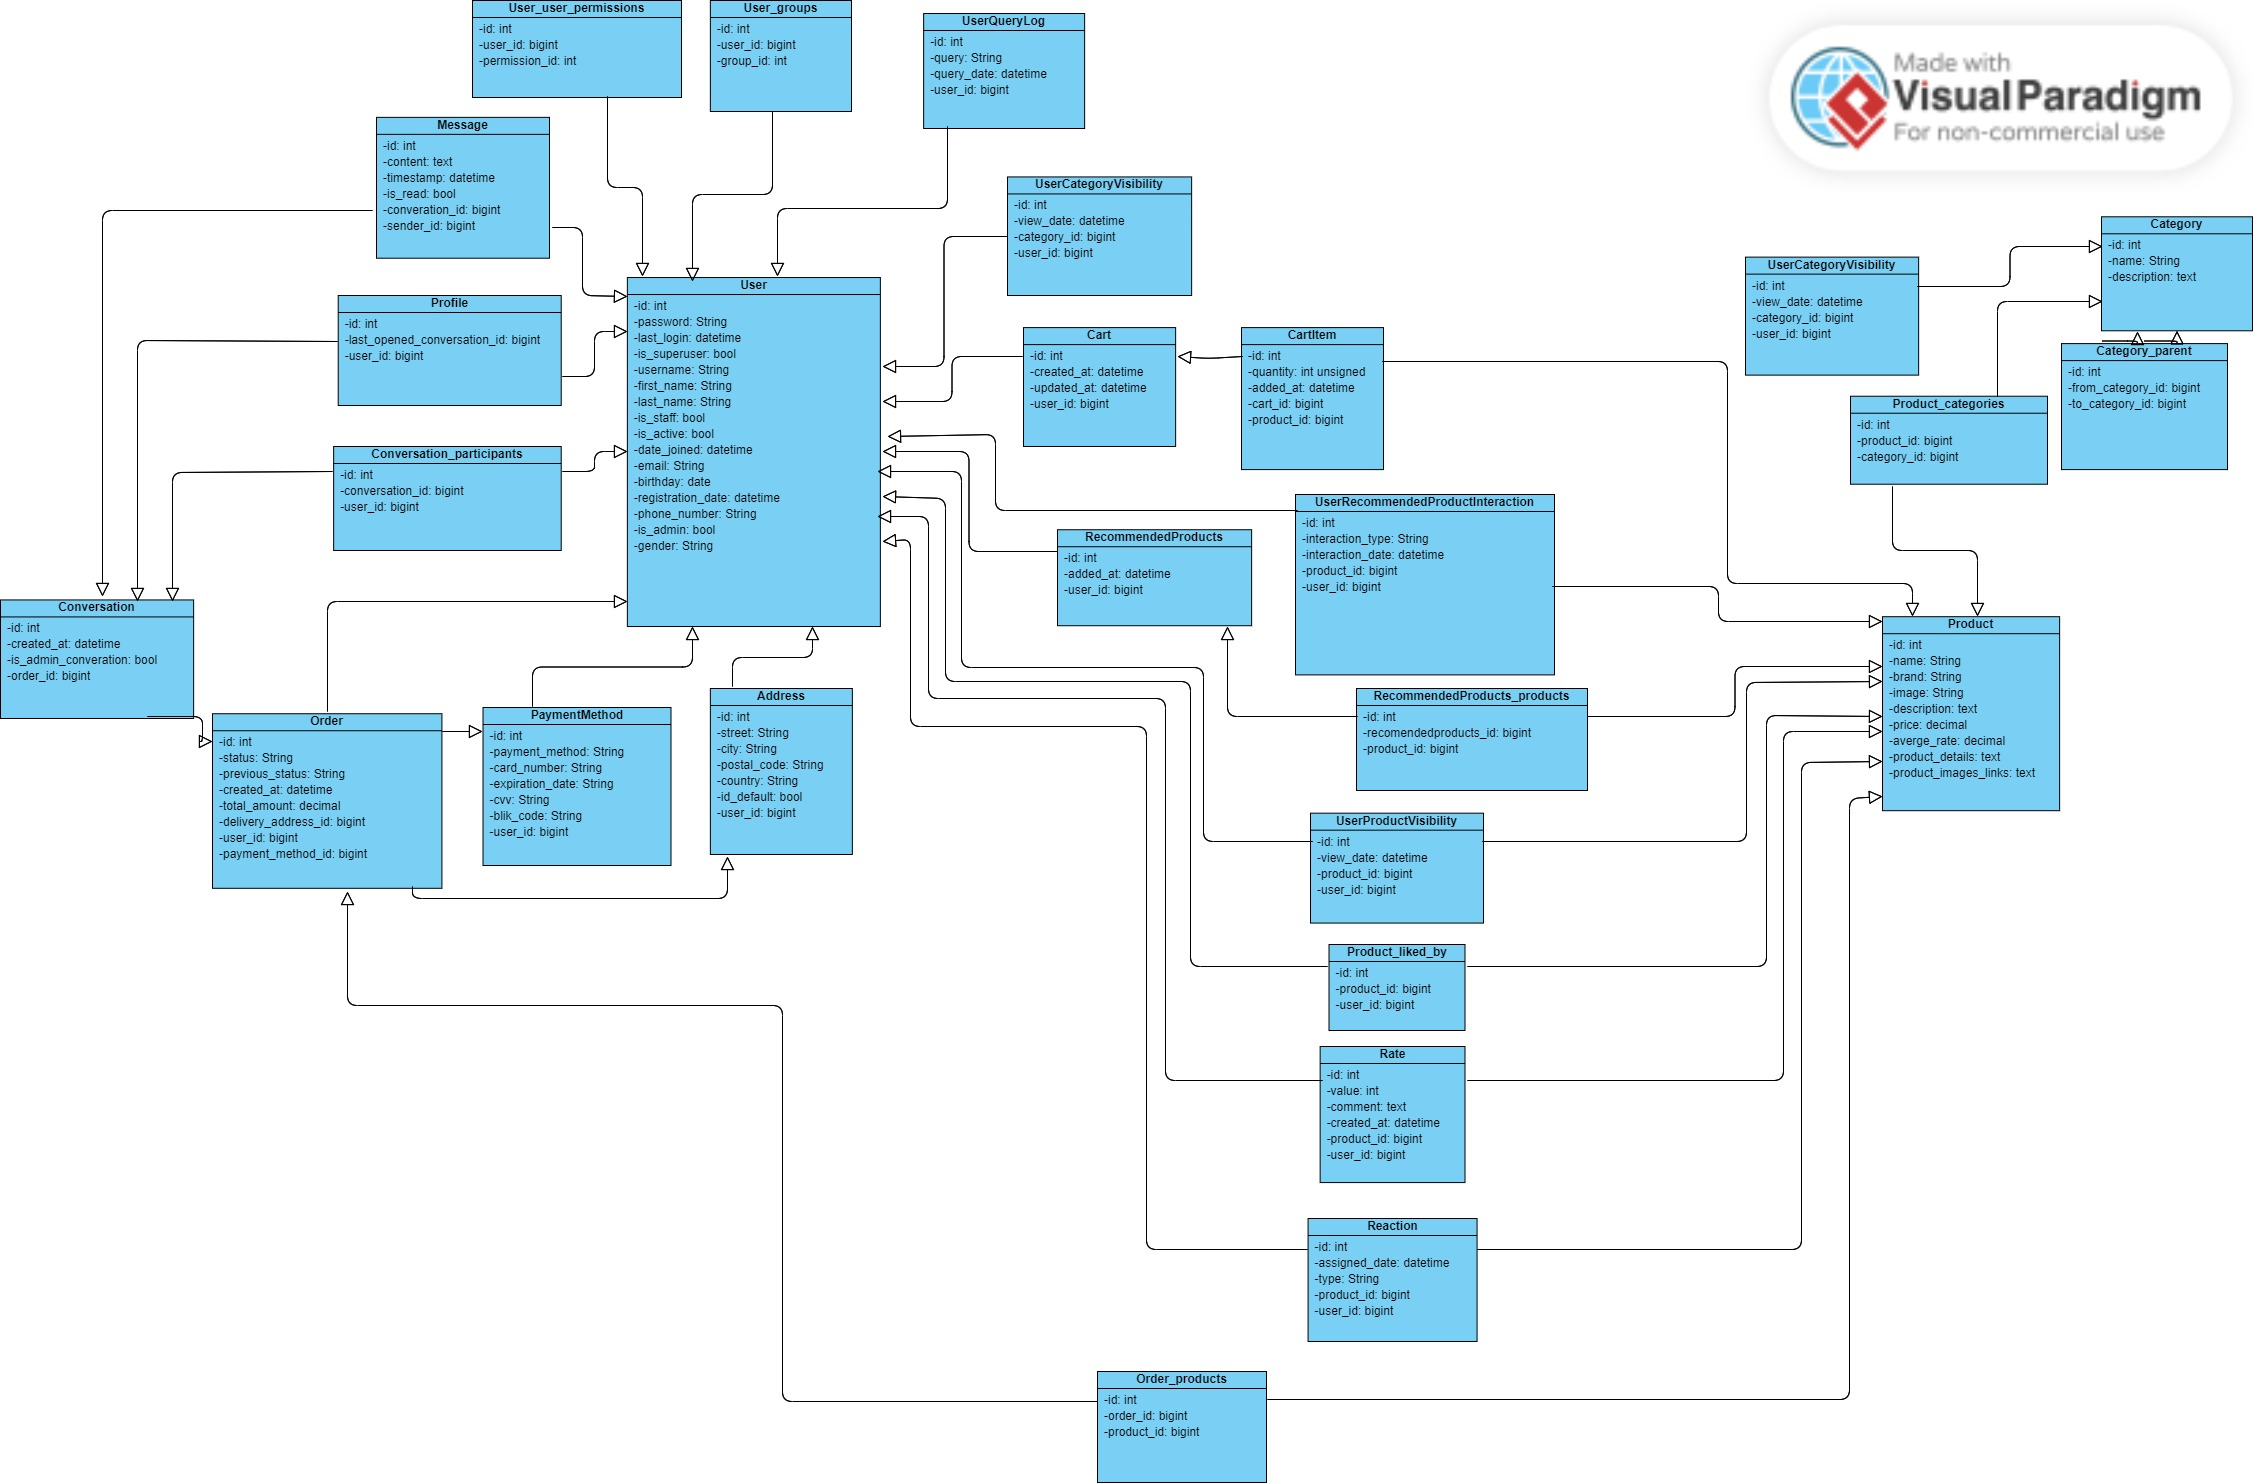
\includegraphics[width=1.0\columnwidth]{images/UML.jpg}
\end{center}

\subsection{Projekt bazy danych}
\subsubsection{Tabele}
\paragraph{Tabela \texttt{Address}}
\subparagraph{Opis:} Przechowuje informacje o adresach użytkowników.
    \begin{itemize}
        \item \texttt{street} : varchar(255) – ulica
        \item \texttt{city} : varchar(100) – miasto
        \item \texttt{postal\string_code} : varchar(20) – kod pocztowy
        \item \texttt{country} : varchar(100) – kraj
        \item \texttt{is\string_default} : bool – flaga domyślnego adresu
        \item \texttt{user\string_id} : bigint (klucz obcy do \texttt{User})
        \item \texttt{id} : integer (klucz główny)
    \end{itemize}

\paragraph{Tabela \texttt{Cart}}
\subparagraph{Opis:} Przechowuje informacje o koszykach zakupowych.
\begin{itemize}
    \item \texttt{created\string_at} : datetime – data utworzenia koszyka
    \item \texttt{updated\string_at} : datetime – data ostatniej aktualizacji
    \item \texttt{user\string_id} : bigint (klucz obcy do \texttt{User})
    \item \texttt{id} : integer (klucz główny)
\end{itemize}

\paragraph{Tabela \texttt{CartItem}}
\subparagraph{Opis:} Przechowuje informacje o produktach w koszyku.
\begin{itemize}
    \item \texttt{quantity} : integer unsigned – ilość produktu
    \item \texttt{added\string_at} : datetime – data dodania produktu
    \item \texttt{cart\string_id} : bigint (klucz obcy do \texttt{Cart})
    \item \texttt{product\string_id} : bigint (klucz obcy do \texttt{Product})
    \item \texttt{id} : integer (klucz główny)
\end{itemize}

\paragraph{Tabela \texttt{Category}}
\subparagraph{Opis:} Przechowuje informacje o kategoriach produktów.
\begin{itemize}
    \item \texttt{name} : varchar(100) – nazwa kategorii
    \item \texttt{description} : text – opis kategorii
    \item \texttt{id} : integer (klucz główny)
\end{itemize}

\paragraph{Tabela \texttt{Category\string_parent}}
\subparagraph{Opis:} Definiuje relacje hierarchiczne między kategoriami.
\begin{itemize}
    \item \texttt{from\string_category\string_id} : bigint (klucz obcy do \texttt{Category})
    \item \texttt{to\string_category\string_id} : bigint (klucz obcy do \texttt{Category})
    \item \texttt{id} : integer (klucz główny)
\end{itemize}

\paragraph{Tabela \texttt{Conversation}}
\subparagraph{Opis:} Przechowuje informacje o rozmowach.
\begin{itemize}
    \item \texttt{created\string_at} : datetime – data utworzenia rozmowy
    \item \texttt{is\string_admin\string_conversation} : bool – flaga rozmowy administracyjnej
    \item \texttt{order\string_id} : bigint (klucz obcy do \texttt{Order})
    \item \texttt{id} : integer (klucz główny)
\end{itemize}

\paragraph{Tabela \texttt{Conversation\string_participants}}
\subparagraph{Opis:} Przechowuje uczestników rozmowy.
\begin{itemize}
    \item \texttt{conversation\string_id} : bigint (klucz obcy do \texttt{Conversation})
    \item \texttt{user\string_id} : bigint (klucz obcy do \texttt{User})
    \item \texttt{id} : integer (klucz główny)
\end{itemize}

\paragraph{Tabela \texttt{Message}}
\subparagraph{Opis:} Przechowuje wiadomości w rozmowach.
\begin{itemize}
    \item \texttt{content} : text – treść wiadomości
    \item \texttt{timestamp} : datetime – znacznik czasu wiadomości
    \item \texttt{is\string_read} : bool – flaga odczytania wiadomości
    \item \texttt{conversation\string_id} : bigint (klucz obcy do \texttt{Conversation})
    \item \texttt{sender\string_id} : bigint (klucz obcy do \texttt{User})
    \item \texttt{id} : integer (klucz główny)
\end{itemize}

\paragraph{Tabela \texttt{Order}}
\subparagraph{Opis:} Przechowuje informacje o zamówieniach.
\begin{itemize}
    \item \texttt{status} : varchar(20) – status zamówienia
    \item \texttt{previous\string_status} : varchar(20) – poprzedni status
    \item \texttt{created\string_at} : datetime – data utworzenia
    \item \texttt{total\string_amount} : decimal – łączna kwota
    \item \texttt{delivery\string_address\string_id} : bigint (klucz obcy do \texttt{Address})
    \item \texttt{user\string_id} : bigint (klucz obcy do \texttt{User})
    \item \texttt{payment\string_method\string_id} : bigint (klucz obcy do \texttt{PaymentMethod})
    \item \texttt{id} : integer (klucz główny)
\end{itemize}

\paragraph{Tabela \texttt{PaymentMethod}}
\subparagraph{Opis:} Przechowuje informacje o metodach płatności.
\begin{itemize}
    \item \texttt{payment\string_method} : varchar(20) – typ metody
    \item \texttt{card\string_number} : varchar(16) – numer karty
    \item \texttt{expiration\string_date} : varchar(5) – data ważności
    \item \texttt{cvv} : varchar(4) – kod CVV
    \item \texttt{blik\string_code} : varchar(6) – kod Blik
    \item \texttt{user\string_id} : bigint (klucz obcy do \texttt{User})
    \item \texttt{id} : integer (klucz główny)
\end{itemize}

\paragraph{Tabela \texttt{Product}}
\subparagraph{Opis:} Przechowuje informacje o produktach.
\begin{itemize}
    \item \texttt{name} : varchar(100) – nazwa produktu
    \item \texttt{brand} : varchar(100) – marka produktu
    \item \texttt{image} : varchar(100) – obraz produktu
    \item \texttt{description} : text – opis produktu
    \item \texttt{price} : decimal – cena produktu
    \item \texttt{average\string_rate} : decimal – średnia ocena
    \item \texttt{product\string_details} : text – szczegóły produktu
    \item \texttt{product\string_images\string_links} : text – linki do zdjęć
    \item \texttt{id} : integer (klucz główny)
\end{itemize}

\paragraph{Tabela \texttt{Order\string_products}}
\subparagraph{Opis:} Przechowuje informacje o produktach w zamówieniach.
\begin{itemize}
    \item \texttt{order\string_id} : bigint (klucz obcy do \texttt{Order})
    \item \texttt{product\string_id} : bigint (klucz obcy do \texttt{Product})
    \item \texttt{id} : integer (klucz główny)
\end{itemize}

\paragraph{Tabela \texttt{Product\string_categories}}
\subparagraph{Opis:} Przechowuje relacje między produktami a kategoriami.
\begin{itemize}
    \item \texttt{product\string_id} : bigint (klucz obcy do \texttt{Product})
    \item \texttt{category\string_id} : bigint (klucz obcy do \texttt{Category})
    \item \texttt{id} : integer (klucz główny)
\end{itemize}

\paragraph{Tabela \texttt{Product\string_liked\string_by}}
\subparagraph{Opis:} Przechowuje informacje o użytkownikach, którzy polubili produkty.
\begin{itemize}
    \item \texttt{product\string_id} : bigint (klucz obcy do \texttt{Product})
    \item \texttt{user\string_id} : bigint (klucz obcy do \texttt{User})
    \item \texttt{id} : integer (klucz główny)
\end{itemize}

\paragraph{Tabela \texttt{RecommendedProducts}}
\subparagraph{Opis:} Przechowuje listy rekomendowanych produktów.
\begin{itemize}
    \item \texttt{added\string_at} : datetime – data dodania listy
    \item \texttt{user\string_id} : bigint (klucz obcy do \texttt{User})
    \item \texttt{id} : integer (klucz główny)
\end{itemize}

\paragraph{Tabela \texttt{RecommendedProducts\string_products}}
\subparagraph{Opis:} Przechowuje produkty powi\k{a}zane z rekomendacjami.
\begin{itemize}
    \item \texttt{RecommendedProducts\string_id} : bigint (klucz obcy do \texttt{RecommendedProducts})
    \item \texttt{product\string_id} : bigint (klucz obcy do \texttt{Product})
    \item \texttt{id} : integer (klucz główny)
\end{itemize}

\paragraph{Tabela \texttt{User\string_groups}}
\subparagraph{Opis:} Przechowuje relacje między użytkownikami a grupami.
\begin{itemize}
    \item \texttt{user\string_id} : bigint (klucz obcy do \texttt{User})
    \item \texttt{group\string_id} : integer (klucz obcy do \texttt{Auth\string_group})
    \item \texttt{id} : integer (klucz główny)
\end{itemize}

\paragraph{Tabela \texttt{UserCategoryVisibility}}
\subparagraph{Opis:} Przechowuje informacje o widoczności kategorii dla użytkowników.
\begin{itemize}
    \item \texttt{view\string_date} : datetime – data widoczności
    \item \texttt{category\string_id} : bigint (klucz obcy do \texttt{Category})
    \item \texttt{user\string_id} : bigint (klucz obcy do \texttt{User})
    \item \texttt{id} : integer (klucz główny)
\end{itemize}

\paragraph{Tabela \texttt{UserQueryLog}}
\subparagraph{Opis:} Przechowuje zapytania wykonane przez użytkowników.
\begin{itemize}
    \item \texttt{query} : varchar(255) – treść zapytania
    \item \texttt{query\string_date} : datetime – data zapytania
    \item \texttt{user\string_id} : bigint (klucz obcy do \texttt{User})
    \item \texttt{id} : integer (klucz główny)
\end{itemize}

\paragraph{Tabela \texttt{Profile}}
\subparagraph{Opis:} Przechowuje informacje o profilach użytkowników.
\begin{itemize}
    \item \texttt{last\string_opened\string_conversation\string_id} : bigint (klucz obcy do \texttt{Conversation})
    \item \texttt{user\string_id} : bigint (klucz obcy do \texttt{User})
    \item \texttt{id} : integer (klucz główny)
\end{itemize}

\paragraph{Tabela \texttt{Rate}}
\subparagraph{Opis:} Przechowuje oceny produktów wystawione przez użytkowników.
\begin{itemize}
    \item \texttt{value} : integer – wartość oceny
    \item \texttt{comment} : text – komentarz do oceny
    \item \texttt{created\string_at} : datetime – data wystawienia oceny
    \item \texttt{product\string_id} : bigint (klucz obcy do \texttt{Product})
    \item \texttt{user\string_id} : bigint (klucz obcy do \texttt{User})
    \item \texttt{id} : integer (klucz główny)
\end{itemize}

\paragraph{Tabela \texttt{Reaction}}
\subparagraph{Opis:} Przechowuje reakcje użytkowników na produkty.
\begin{itemize}
    \item \texttt{assigned\string_date} : datetime – data przypisania reakcji
    \item \texttt{type} : varchar(10) – typ reakcji (np. „like” lub „dislike”)
    \item \texttt{product\string_id} : bigint (klucz obcy do \texttt{Product})
    \item \texttt{user\string_id} : bigint (klucz obcy do \texttt{User})
    \item \texttt{id} : integer (klucz główny)
\end{itemize}

\paragraph{Tabela \texttt{UserProductVisibility}}
\subparagraph{Opis:} Przechowuje informacje o widoczności produktów dla użytkowników.
\begin{itemize}
    \item \texttt{view\string_date} : datetime – data widoczności
    \item \texttt{product\string_id} : bigint (klucz obcy do \texttt{Product})
    \item \texttt{user\string_id} : bigint (klucz obcy do \texttt{User})
    \item \texttt{id} : integer (klucz główny)
\end{itemize}

\paragraph{Tabela \texttt{UserRecommendedProductInteraction}}
\subparagraph{Opis:} Przechowuje informacje o interakcjach użytkowników z rekomendowanymi produktami.
\begin{itemize}
    \item \texttt{interaction\string_type} : varchar(20) – typ interakcji (np. kliknięcie, zakup)
    \item \texttt{interaction\string_date} : datetime – data interakcji
    \item \texttt{product\string_id} : bigint (klucz obcy do \texttt{Product})
    \item \texttt{user\string_id} : bigint (klucz obcy do \texttt{User})
    \item \texttt{id} : integer (klucz główny)
\end{itemize}

\paragraph{Tabela \texttt{User\string_user\string_permissions}}
\subparagraph{Opis:} Przechowuje informacje o uprawnieniach użytkowników.
\begin{itemize}
    \item \texttt{user\string_id} : bigint (klucz obcy do \texttt{User})
    \item \texttt{permission\string_id} : integer (klucz obcy do \texttt{Auth\string_permission})
    \item \texttt{id} : integer (klucz główny)
\end{itemize}

\paragraph{Tabela \texttt{User\string_query\string_log}}
\subparagraph{Opis:} Przechowuje zapytania wyszukiwania wykonane przez użytkowników.
\begin{itemize}
    \item \texttt{query} : varchar(255) – treść zapytania
    \item \texttt{query\string_date} : datetime – data zapytania
    \item \texttt{user\string_id} : bigint (klucz obcy do \texttt{User})
    \item \texttt{id} : integer (klucz główny)
\end{itemize}


\subsubsection{Relacje między tabelami}
\begin{itemize}
    \item \texttt{Address.user\string_id} $\to$ \texttt{User.id}
    \item \texttt{Cart.user\string_id} $\to$ \texttt{User.id}
    \item \texttt{CartItem.cart\string_id} $\to$ \texttt{Cart.id}
    \item \texttt{CartItem.product\string_id} $\to$ \texttt{Product.id}
    \item \texttt{Category\string_parent.from\string_category\string_id} $\to$ \texttt{Category.id}
    \item \texttt{Category\string_parent.to\string_category\string_id} $\to$ \texttt{Category.id}
    \item \texttt{Conversation.order\string_id} $\to$ \texttt{Order.id}
    \item \texttt{Conversation\string_participants.conversation\string_id} $\to$ \texttt{Conversation.id}
    \item \texttt{Conversation\string_participants.user\string_id} $\to$ \texttt{User.id}
    \item \texttt{Message.conversation\string_id} $\to$ \texttt{Conversation.id}
    \item \texttt{Message.sender\string_id} $\to$ \texttt{User.id}
    \item \texttt{Order\string_products.order\string_id} $\to$ \texttt{Order.id}
    \item \texttt{Order\string_products.product\string_id} $\to$ \texttt{Product.id}
    \item \texttt{Product\string_categories.product\string_id} $\to$ \texttt{Product.id}
    \item \texttt{Product\string_categories.category\string_id} $\to$ \texttt{Category.id}
    \item \texttt{Product\string_liked\string_by.product\string_id} $\to$ \texttt{Product.id}
    \item \texttt{Product\string_liked\string_by.user\string_id} $\to$ \texttt{User.id}
    \item \texttt{RecommendedProducts\string_products.recommendedproducts\string_id} $\to$ \texttt{RecommendedProducts.id}
    \item \texttt{RecommendedProducts\string_products.product\string_id} $\to$ \texttt{Product.id}
    \item \texttt{User\string_groups.user\string_id} $\to$ \texttt{User.id}
    \item \texttt{UserCategoryVisibility.category\string_id} $\to$ \texttt{Category.id}
    \item \texttt{Profile.last\string_opened\string_conversation\string_id} $\to$ \texttt{Conversation.id}
    \item \texttt{Rate.product\string_id} $\to$ \texttt{Product.id}
    \item \texttt{Rate.user\string_id} $\to$ \texttt{User.id}
    \item \texttt{Reaction.product\string_id} $\to$ \texttt{Product.id}
    \item \texttt{Reaction.user\string_id} $\to$ \texttt{User.id}
    \item \texttt{UserRecommendedProductInteraction.product\string_id} $\to$ \texttt{Product.id}
    \item \texttt{UserRecommendedProductInteraction.user\string_id} $\to$ \texttt{User.id}
\end{itemize}


\subsubsection{Przykładowe procedury składowane}
\paragraph{Dodawanie nowego użytkownika}
    \begin{verbatim}
    CREATE OR REPLACE PROCEDURE add_user(
        p_username VARCHAR,
        p_email VARCHAR,
        p_password VARCHAR
    )
    BEGIN
        INSERT INTO User (username, email, password)
        VALUES (p_username, p_email, p_password);
    END;
    \end{verbatim}

\paragraph{Pobieranie zamówień użytkownika}
    \begin{verbatim}
    CREATE OR REPLACE FUNCTION get_user_orders(p_user_id INT)
    RETURNS TABLE(order_id INT, order_date DATETIME, status VARCHAR)
    BEGIN
        RETURN QUERY
        SELECT id, order_date, status
        FROM Order
        WHERE user_id = p_user_id;
    END;
    \end{verbatim}

\clearpage

\section{Szczegółowa dokumentacja kodu}
Poniżej przedstawiono szczegółową dokumentację dotyczącą implementacji aplikacji.
%
%  model User
%
\subsection{Model \texttt{User}}
\textbf{Opis:} 
Model \texttt{User} rozszerza wbudowany model \texttt{AbstractUser} i przechowuje informacje o użytkownikach systemu, takie jak dane personalne, datę rejestracji, numer telefonu oraz płeć. Wprowadza dodatkowe pola, które uzupełniają funkcjonalności dziedziczone z \texttt{AbstractUser}.

\subsubsection{Pola modelu \texttt{User}}
\begin{itemize}
    \item \texttt{email}: \texttt{EmailField} – unikalny adres e-mail użytkownika (nadpisuje pole z \texttt{AbstractUser}).
    \item \texttt{birthday}: \texttt{DateField} – data urodzenia użytkownika (opcjonalne).
    \item \texttt{registration\_date}: \texttt{DateTimeField} – data rejestracji użytkownika (domyślnie ustawiana na bieżącą datę i czas).
    \item \texttt{phone\_number}: \texttt{CharField} – numer telefonu użytkownika (wymagane, maksymalnie 15 znaków).
    \item \texttt{is\_admin}: \texttt{BooleanField} – flaga wskazująca, czy użytkownik jest administratorem.
    \item \texttt{gender}: \texttt{CharField} – płeć użytkownika, wybierana spośród wartości:
    \begin{itemize}
        \item \texttt{Male}
        \item \texttt{Female}
        \item \texttt{Other}
    \end{itemize}
\end{itemize}

\textbf{Najważniejsze pola dziedziczone z modelu \texttt{AbstractUser}:}
\begin{itemize}
    \item \texttt{password}: \texttt{CharField} – hasło użytkownika (zabezpieczone poprzez funkcję \texttt{set\_password}).
    \item \texttt{is\_superuser}: \texttt{BooleanField} – flaga oznaczająca, czy użytkownik jest superużytkownikiem.
    \item \texttt{username}: \texttt{CharField} – unikalna nazwa użytkownika.
    \item \texttt{is\_active}: \texttt{BooleanField} – flaga wskazująca, czy konto użytkownika jest aktywne.
\end{itemize}

\subsubsection{Kod modelu}
\begin{lstlisting}[language=Python, caption=Model \texttt{User}]
class User(AbstractUser):
    email = models.EmailField(unique=True)
    birthday = models.DateField(null=True, blank=True)
    registration_date = models.DateTimeField(default=timezone.now)
    phone_number = models.CharField(max_length=15, null=False, blank=False)
    is_admin = models.BooleanField(default=False)
    gender = models.CharField(
        max_length=10, choices=[(gender.value, gender.name.capitalize()) for gender in UserGender],
        default=UserGender.MALE.value
    )
\end{lstlisting}


\subsubsection{Formularze użytkownika}
\linespread{1.3}
\subsubsection*{Formularz rejestracji (\texttt{UserRegistrationForm})}

\textbf{Opis:}
Formularz obsługujący rejestrację użytkownika w systemie. Oprócz standardowych pól takich jak imię, nazwisko czy hasło, zawiera dodatkową walidację dla numeru telefonu oraz adresu e-mail.

--

\textbf{Pola formularza:}
\begin{itemize}
    \item \texttt{first\_name}, \texttt{last\_name}, \texttt{email}, \texttt{phone\_number}, \texttt{birthday}, \texttt{gender}, \texttt{password}.
\end{itemize}

\textbf{Metody walidacji:}
\begin{itemize}
    \item \texttt{clean\_email}: Sprawdza, czy podany adres e-mail jest unikalny oraz należy do poprawnej domeny.
\begin{lstlisting}[language=Python]
if User.objects.filter(email=email).exists():
    raise forms.ValidationError("Email is already taken")
elif not email.endswith((".com", ".org", ".edu")):
    raise forms.ValidationError("Invalid email domain")
\end{lstlisting}
    \item \texttt{clean\_phone\_number}: Weryfikuje, czy numer telefonu zawiera dokładnie 9 cyfr.
\begin{lstlisting}[language=Python]
parsed_phone_number = re.sub(r'\D', '', phone_number)
if len(parsed_phone_number) != 9:
    raise ValidationError("Phone number must have exactly 9 digits.")
\end{lstlisting}
\end{itemize}

\textbf{Metoda zapisu:}
\begin{itemize}
    \item \texttt{save()}: Tworzy nowego użytkownika, ustawiając dla niego unikalne hasło i nazwę użytkownika.
\end{itemize}

\subsubsection*{Formularz logowania (\texttt{UserLoginForm})}

\textbf{Opis:}
Formularz umożliwiający logowanie użytkownika w systemie. Waliduje poprawność podanych danych logowania.

\textbf{Pola formularza:}
\begin{itemize}
    \item \texttt{email}, \texttt{password}.
\end{itemize}

\subsubsection{Widoki modelu \texttt{User}}

\subsubsection*{Widok rejestrowania \texttt{UserRegisterView}}
\begin{itemize}
    \item \textbf{Opis:}
        Widok umożliwiający rejestrację nowego użytkownika w systemie. Obsługuje walidację danych wprowadzonych w formularzu rejestracyjnym, zapisuje nowego użytkownika w bazie danych oraz przekierowuje na stronę logowania po pomyślnym zarejestrowaniu.
    \item \textbf{Formularz:}
        \texttt{UserRegistrationForm} (opisany w sekcji \texttt{Formularz rejestracji}).
    \item \textbf{Szablon:}
        (\texttt{"registration/register.html"})
        \subsubitem Kod szablonu został szczegółowo opisany w sekcji \ref{sec:register_template}
    \item \textbf{Atrybuty:}
        \begin{itemize}
            \item \texttt{template\_name:} Ścieżka do szablonu używanego w widoku (\texttt{"registration/register.html"}).
            \item \texttt{form\_class:} Formularz powiązany z widokiem (\texttt{UserRegistrationForm}).
            \item \texttt{success\_url:} URL, na który użytkownik jest przekierowywany po pomyślnej rejestracji (\texttt{"login"}).
        \end{itemize}
    \item \textbf{Metody:}
        \begin{itemize}
            \item \texttt{form\_valid(self, form):}
                \begin{itemize}
                    \item \textbf{Opis:} Zapisuje dane nowego użytkownika i przekierowuje na stronę logowania.
                    \item \textbf{Kod:}
                    \begin{lstlisting}[language=Python, caption=Metoda form\_valid w UserRegisterView]
def form_valid(self, form):
    user = form.save(commit=True)
    messages.success(self.request, "Registration successful. Please log in.")
    send_registration_email(user.email, user)
    return super().form_valid(form)
                    \end{lstlisting}
                \end{itemize}
        \end{itemize}
\end{itemize}

\subsubsection*{Widok logowania (\texttt{UserLoginView})}

\textbf{Opis:}
Widok umożliwiający logowanie użytkownika do systemu na podstawie formularza logowania. Obsługuje uwierzytelnianie oraz przekierowanie po pomyślnym zalogowaniu.

--

\textbf{Atrybuty:}
\begin{itemize}
    \item \texttt{template\_name}: Ścieżka do szablonu logowania (\texttt{"registration/login.html"}).
    \subsubitem Kod szablonu został szczegółowo opisany w sekcji \ref{sec:login_template}.

    \item \texttt{form\_class}: Klasa formularza używanego w widoku (\texttt{UserLoginForm}).
    \item \texttt{success\_url}: URL przekierowania po zalogowaniu (\texttt{home}).
\end{itemize}


\textbf{Metody:}
\begin{itemize}
    \item \texttt{form\_valid(self, form)}:
    \begin{itemize}
        \item \textbf{Opis:} Obsługuje poprawne przesłanie formularza logowania.
        \item \textbf{Kod:}
        \begin{lstlisting}[language=Python, caption=Metoda form\_valid w UserLoginView]
def form_valid(self, form):
    email = form.cleaned_data.get('email')
    password = form.cleaned_data.get('password')
    try:
        user = User.objects.get(email=email)
        username = user.username
        user = authenticate(self.request, username=username, password=password)
        if user is not None:
            login(self.request, user)
            messages.success(self.request, "Login successfully")
            sync_session_likes_to_user(self.request)
            return super().form_valid(form)
        else:
            form.add_error(None, "Incorrect email or password")
    except User.DoesNotExist:
        form.add_error('email', "No user found with the given email address")
    return self.form_invalid(form)
        \end{lstlisting}
        \item \textbf{Wyjaśnienie:}
        \begin{itemize}
            \item Pobiera dane logowania z formularza (\texttt{email}, \texttt{password}).
            \item Wyszukuje użytkownika na podstawie podanego adresu e-mail.
            \item Próbuje uwierzytelnić użytkownika za pomocą funkcji \texttt{authenticate}.
            \item Jeśli uwierzytelnienie powiedzie się, loguje użytkownika i wyświetla komunikat o sukcesie.
            \item Jeśli uwierzytelnienie nie powiedzie się, dodaje odpowiednie błędy do formularza.
        \end{itemize}
    \end{itemize}

    \item \texttt{form\_invalid(self, form)}:
    \begin{itemize}
        \item \textbf{Opis:} Obsługuje przypadki, gdy formularz logowania jest niepoprawny.
        \item \textbf{Kod:}
        \begin{lstlisting}[language=Python, caption=Metoda \texttt{form\_invalid} w UserLoginView]
def form_invalid(self, form):
    return super().form_invalid(form)
        \end{lstlisting}
        \item \textbf{Wyjaśnienie:}
        \begin{itemize}
            \item Przekazuje błędne dane do szablonu w celu wyświetlenia odpowiednich komunikatów błędów.
        \end{itemize}
    \end{itemize}
\end{itemize}

\subsubsection*{Widok wylogowania (\texttt{logout\_view})}
\begin{itemize}
    \item \texttt{logout\_view}:
    \begin{itemize}
        \item \textbf{Opis:} Widok odpowiedzialny za wylogowanie użytkownika i przekierowanie go na stronę główną aplikacji.
        \item \textbf{Kod:}
        \begin{lstlisting}[language=Python, caption=Widok \texttt{logout\_view}]
@login_required
def logout_view(request):
    logout(request)
    messages.success(request, "Logout successfully")
    return redirect("home")
        \end{lstlisting}
        \item \textbf{Wyjaśnienie:}
        \begin{itemize}
            \item Sprawdza, czy użytkownik jest zalogowany (\texttt{@login\_required}).
            \item Wylogowuje użytkownika za pomocą funkcji \texttt{logout}.
            \item Wyświetla komunikat potwierdzający wylogowanie.
            \item Przekierowuje użytkownika na stronę główną (\texttt{"home"}).
        \end{itemize}
    \end{itemize}
\end{itemize}


\subsubsection{Endpointy użytkownika}

\begin{itemize}
    \item \texttt{/register/}: Rejestracja użytkownika (\texttt{UserRegisterView}).
    \item \texttt{/login/}: Logowanie użytkownika (\texttt{UserLoginView}).
    \item \texttt{/logout/}: Wylogowanie użytkownika (\texttt{logout\_view}).
\end{itemize}

\textbf{Przykład zapytania POST:}
\begin{verbatim}
        POST /login/
        Body: {
            "email": "example@example.com",
            "password": "securepassword"
        }
        Response: 200 OK
\end{verbatim}
\subsubsection{Szablony użytkownika}

\subsubsection*{\texttt{login.html}}
\label{sec:login_template}

Szablon odpowiedzialny za logowanie użytkownika do systemu. Formularz zawiera pola dla adresu e-mail oraz hasła, które są walidowane i przesyłane do widoku obsługującego logowanie.

\textbf{Kod szablonu:}
\begin{lstlisting}[language=HTML, caption=Szablon \texttt{login.html}]
<form method="post" action="">
    
    <label for="id_email">Email:</label>
    <input type="email" name="email" id="id_email" required>
    <label for="id_password">Haslo:</label>
    <input type="password" name="password" id="id_password" required>
    <button type="submit">Zaloguj sie</button>
</form>
\end{lstlisting}

\textbf{Wyjaśnienie:}
\begin{itemize}
    \item \texttt{method="post"}: Formularz przesyła dane przy użyciu metody HTTP POST.
    \item \texttt{{\% csrf\_token \%}}: Token CSRF zapewniający ochronę przed atakami Cross-Site Request Forgery (wymagany w Django).
    \item \texttt{name="email"}: Pole tekstowe umożliwiające wpisanie adresu e-mail użytkownika.
    \item \texttt{name="password"}: Pole tekstowe umożliwiające wpisanie hasła użytkownika.
    \item Przycisk \texttt{submit}: Służy do przesłania danych formularza do widoku logowania.
\end{itemize}

\subsubsection*{\texttt{register.html}}
\label{sec:register_template}

Szablon odpowiedzialny za rejestrację nowych użytkowników. Formularz pozwala na wprowadzenie danych takich jak imię, nazwisko, adres e-mail, numer telefonu, data urodzenia, płeć i hasło.

\textbf{Kod szablonu:}
\begin{lstlisting}[language=HTML, caption=Szablon \texttt{register.html}]
<form method="post" action="">
    
    <label for="id_first_name">Imie:</label>
    <input type="text" name="first_name" id="id_first_name" required>
    <label for="id_last_name">Nazwisko:</label>
    <input type="text" name="last_name" id="id_last_name" required>
    <label for="id_email">Email:</label>
    <input type="email" name="email" id="id_email" required>
    <button type="submit">Zarejestruj sie</button>
</form>
\end{lstlisting}

\textbf{Wyjaśnienie:}
\begin{itemize}
    \item \texttt{name="first\_name"}: Pole do wprowadzenia imienia użytkownika.
    \item \texttt{name="last\_name"}: Pole do wprowadzenia nazwiska użytkownika.
    \item \texttt{name="email"}: Pole do wprowadzenia adresu e-mail użytkownika.
    \item \texttt{{\% csrf\_token \%}}: Zabezpieczenie przed atakami CSRF, standardowe w Django.
    \item Przycisk \texttt{submit}: Wysyła dane formularza do widoku obsługującego rejestrację.
\end{itemize}

\textbf{Uwagi:}
\begin{itemize}
    \item Oba szablony wykorzystują prostą strukturę HTML, co zapewnia przejrzystość i łatwość obsługi.
    \item Zabezpieczenie CSRF (Cross-Site Request Forgery) jest stosowane w obu przypadkach w celu ochrony danych użytkownika.
    \item Formularze mogą być rozszerzone o dodatkowe style CSS lub framework (np. Bootstrap) w dalszym etapie rozwoju aplikacji.
\end{itemize}

\subsubsection{Funkcje pomocnicze}
\label{sec:helper_functions}

\subsubsection*{\texttt{send\_registration\_email(email, user)}}
Funkcja pomocnicza odpowiedzialna za wysyłanie wiadomości e-mail potwierdzających rejestrację nowego użytkownika w systemie.

--

\textbf{Kod funkcji:}
\begin{lstlisting}[language=Python, caption=Funkcja \texttt{send\_registration_email}]
def send_registration_email(email, user):
    subject = 'Rejestracja w KMG Store'
    html_message = render_to_string('email/registration_email.html', {'user': user})
    plain_message = strip_tags(html_message)
    from_email = 'kmgstoreproject@gmail.com'
    to = email

    send_mail(subject, plain_message, from_email, [to], html_message=html_message)
\end{lstlisting}

\textbf{Opis działania:}
\begin{itemize}
    \item Pobiera adres e-mail oraz obiekt użytkownika jako parametry wejściowe.
    \item Generuje temat wiadomości (\texttt{subject}) oraz treść HTML za pomocą szablonu \texttt{registration\_email.html}.
    \item Wysyła wiadomość e-mail za pomocą funkcji \texttt{send\_mail} z pakietu Django.
\end{itemize}

\textbf{Uwagi:}
\begin{itemize}
    \item Funkcja korzysta z szablonu wiadomości e-mail w celu zapewnienia spójnego wyglądu wiadomości wysyłanych do użytkowników.
    \item Adres nadawcy (\texttt{from\_email}) można zmodyfikować w plikach konfiguracyjnych aplikacji Django.
\end{itemize}

\subsubsection*{Zastosowane wzorce projektowe}
\begin{itemize}
    \item \textbf{Template Method:} Widoki \texttt{UserRegisterView} i \texttt{UserLoginView} korzystają z generycznych klas widoków Django, pozwalając na definiowanie niestandardowych zachowań za pomocą metod takich jak \texttt{form\_valid}.
    \item \textbf{Factory:} Metoda \texttt{generate\_username} w formularzu rejestracji dynamicznie generuje unikalną nazwę użytkownika na podstawie jego imienia i nazwiska.
\end{itemize}


%
% Model Address
%
\subsection{Model \texttt{Address}}

\textbf{Opis:}  
Model \texttt{Address} przechowuje informacje o adresach użytkowników w systemie. Każdy adres jest powiązany z użytkownikiem i może być oznaczony jako domyślny do użycia w zamówieniach.

\paragraph{Atrybuty:}
\begin{itemize}
    \item \texttt{user}: \texttt{ForeignKey} – Relacja z modelem \texttt{User}.
    \begin{itemize}
        \item \texttt{on\_delete=models.CASCADE} – Usunięcie użytkownika powoduje usunięcie jego adresów.
        \item \texttt{related\_name='addresses'} – Pozwala na dostęp do adresów za pomocą \texttt{user.addresses}.
    \end{itemize}
    \item \texttt{street}: \texttt{CharField} (max. 255 znaków) – Ulica.
    \item \texttt{city}: \texttt{CharField} (max. 100 znaków) – Miasto.
    \item \texttt{postal\_code}: \texttt{CharField} (max. 20 znaków) – Kod pocztowy.
    \item \texttt{country}: \texttt{CharField} (max. 100 znaków) – Kraj.
    \item \texttt{is\_default}: \texttt{BooleanField} – Czy adres jest domyślny (domyślnie: \texttt{False}).
\end{itemize}

\subsubsection{Metody modelu:}
\begin{itemize}
    \item \texttt{get\_address(self)}  
        \begin{itemize}
            \item \textbf{Opis:} Zwraca pełny adres jako łańcuch tekstowy.
            \item \textbf{Kod:}
            \begin{lstlisting}[language=Python, caption=Metoda \texttt{get\_address}]
def get_address(self):
    return f"{self.street}, {self.city}, {self.country}"
            \end{lstlisting}
        \end{itemize}
\end{itemize}


\subsubsection{Formularze adresu}
\linespread{1.3}
\subsubsection*{Formularz \texttt{UserAddressForm}}


\textbf{Opis:}
Formularz umożliwiający użytkownikom dodawanie nowych adresów.

\paragraph{Walidacja pól:}
\begin{itemize}
    \item Sprawdza, czy pola \texttt{street}, \texttt{city}, \texttt{postal\_code} i \texttt{country} są wypełnione.
    \item Umożliwia oznaczenie adresu jako domyślnego.
\end{itemize}

\textbf{Kod walidacji:}
\begin{lstlisting}[language=Python, caption=Walidacja formularza \texttt{UserAddressForm}]
def clean(self):
    cleaned_data = super().clean()
    if not cleaned_data.get('street'):
        self.add_error('street', "Ulica jest wymagana.")
    if not cleaned_data.get('city'):
        self.add_error('city', "Miasto jest wymagane.")
    if not cleaned_data.get('postal_code'):
        self.add_error('postal_code', "Kod pocztowy jest wymagany.")
    if not cleaned_data.get('country'):
        self.add_error('country', "Kraj jest wymagany.")
    return cleaned_data
\end{lstlisting}



\subsubsection{Widoki modelu address}

\subsubsection*{Widok dodawania adresu (\texttt{UserAddressCreationView})}
\begin{itemize}
    \item \textbf{Opis:} Widok umożliwiający użytkownikowi dodanie nowego adresu.
    \item \textbf{Działanie:}
        \begin{itemize}
            \item Obsługuje przesłanie danych z formularza.
            \item Ustawia nowo dodany adres jako domyślny, jeśli wybrano taką opcję.
            \item Po zapisaniu adresu przekierowuje użytkownika do widoku wyboru adresu.
        \end{itemize}
    \item \textbf{Kod metody \texttt{form\_valid}:}
    \begin{lstlisting}[language=Python, caption=Obsługa poprawnego formularza w \texttt{UserAddressCreationView}]
    def form_valid(self, form):
        address = form.save(commit=False)
        address.user = self.request.user

        if form.cleaned_data.get('is_default'):
            Address.objects.filter(user=self.request.user, is_default=True).update(is_default=False)
            address.is_default = True

        address.save()
        messages.success(self.request, f"Adres {address.street} zostal zapisany.")
        return super().form_valid(form)
    \end{lstlisting}
\end{itemize}


\subsubsection*{Widok wyboru adresu (\texttt{AddressSelectionView})}
\begin{itemize}
    \item \textbf{Opis:} Widok prezentujący użytkownikowi listę zapisanych adresów i umożliwiający wybór jednego z nich jako domyślnego.
    \item \textbf{Działanie:}
    \begin{itemize}
        \item Wyświetla listę zapisanych adresów.
        \item Obsługuje oznaczanie adresu jako domyślnego.
        \item Przekierowuje użytkownika do formularza płatności po wyborze adresu.
    \end{itemize}
    \item \textbf{Kod metody \texttt{get}:}
    \begin{lstlisting}[language=Python, caption=Metoda \texttt{get} w \texttt{AddressSelectionView}]
        def get(self, request, *args, **kwargs):
            user_addresses = Address.objects.filter(user=request.user)

            if not user_addresses.exists():
                messages.info(request, "Nie masz jeszcze zapisanych adresow. Dodaj nowy adres.")
                return redirect('add_address')

            default_address = user_addresses.filter(is_default=True).first()
            context = {
                'addresses': user_addresses,
                'default_address_id': default_address.id if default_address else None,
            }
            return render(request, self.template_name, context)
        \end{lstlisting}

\end{itemize}



\subsubsection{Szablony użytkownika}

\subsubsection*{\texttt{add\_address.html}}
\label{sec:add_address_template}
\begin{itemize}
    \item \textbf{Opis:} Szablon umożliwiający dodanie nowego adresu użytkownika.
    \item \textbf{Działanie:}
    \begin{itemize}
        \item Formularz umożliwia użytkownikowi wprowadzenie danych adresowych, takich jak ulica, miasto, kod pocztowy i kraj.
        \item Opcjonalnie użytkownik może oznaczyć adres jako domyślny.
        \item Przyciski nawigacyjne pozwalają zapisać adres lub powrócić do poprzedniego widoku.
    \end{itemize}

    \item \textbf{Kod szablonu:}
\begin{lstlisting}[language=HTML, caption=Szablon add\_address.html]
<form method="post">
    
    
        <div class="form-group">
            <label for="{{ field.name }}" class="form-label">{{ field.label }}:</label>
            <input type="text" id="{{ field.name }}" name="{{ field.name }}" class="form-input"
                placeholder="{{ field.placeholder }}" required>
        </div>
    
    <div class="form-group">
        <label>
            <input type="checkbox" id="is_default" name="is_default" class="form-checkbox">
            Ustaw jako domyslny adres
        </label>
    </div>
    <div class="card">
        <div class="card-body d-flex justify-content-between align-items-center">
            <a href=""
               class="form-button form-button-secondary">Powrot</a>
            <button type="submit" class="btn proceed-button">Zapisz adres</button>
        </div>
    </div>
</form>
\end{lstlisting}
\end{itemize}




\subsubsection*{\texttt{address\_selection.html}}
\label{sec:address_selection_template}
\begin{itemize}
    \item \textbf{Opis:} Szablon umożliwiający wybór istniejącego adresu dostawy.
    \item \textbf{Działanie:}
        \begin{itemize}
            \item Wyświetla listę zapisanych adresów użytkownika jako opcje do wyboru.
            \item Oznacza domyślny adres, jeśli istnieje.
            \item Umożliwia zapisanie wybranego adresu jako domyślnego.
            \item Przycisk nawigacyjny pozwala dodać nowy adres.
        \end{itemize}
    \item \textbf{Kod szablonu:}
\begin{lstlisting}[language=HTML, caption=Szablon address\_selection.html]
<form method="post">
    
    
        <div class="address-card-wrapper address-default">
            <input type="radio" name="selected_address" value="{{ address.id }}" id="address-{{ address.id }}"
                    class="address-card-radio" checked>
            <label for="address-{{ address.id }}" class="address-card-label">
                <div class="address-card-content">
                    <p><strong>{{ address.street }}</strong></p>
                    <p>{{ address.city }}, {{ address.postal_code }}</p>
                    <p>{{ address.country }}</p>
                    
                        <span class="address-default-badge">Domyslny</span>
                    
                </div>
            </label>
        </div>
    
    <div class="card">
        <div class="card-body d-flex justify-content-between align-items-center">
            <a href="" class="form-button form-button-secondary">Dodaj nowy adres</a>
            <button type="submit" class="btn proceed-button">Zatwierdz adres</button>
        </div>
    </div>
</form>
<script src="../static/js/manage_address_selection.js"></script>
\end{lstlisting}
\end{itemize}


\subsubsection{Skrypty JavaScript}

\subsubsection*{\texttt{manage.address\_selection.js}}
\begin{itemize}
    \item \textbf{Opis:}Skrypt odpowiedzialny za obsługę interakcji użytkownika z widokiem wyboru adresu dostawy.
    \item \textbf{Działanie:}
        \begin{itemize}
            \item Obsługuje podświetlanie aktywnej opcji adresu przy kliknięciu na kartę adresu.
            \item Sprawdza, czy użytkownik wybrał adres przed wysłaniem formularza – jeżeli nie, wyświetla komunikat o konieczności wyboru adresu.
        \end{itemize}
    \item \textbf{Kod skryptu:}
\begin{lstlisting}[language=JavaScript, caption=Skrypt manage.address\_choice.js]
document.addEventListener('DOMContentLoaded', function () {
    const addressCards = document.querySelectorAll('.address-card');
    const form = document.getElementById('address-form');

    addressCards.forEach(card => {
        card.addEventListener('click', () => {
            addressCards.forEach(c => c.classList.remove('active'));
            card.classList.add('active');
        });
    });

    form.addEventListener('submit', function (event) {
        const selectedAddress = document.querySelector('input[name="selected_address"]:checked');
        if (!selectedAddress) {
            event.preventDefault();
            alert('Prosze wybrac adres dostawy.');
        }
    });
});
\end{lstlisting}
\end{itemize}


% 
% Model PaymentMethod
% 
\clearpage
\subsection{Model \texttt{PaymentMethod}}

\textbf{Opis:}  
Model \texttt{PaymentMethod} reprezentuje informacje o metodach płatności dostępnych dla użytkowników systemu. Pozwala na przechowywanie szczegółów dotyczących różnych metod płatności, takich jak karta kredytowa, Blik czy płatność za pobraniem. Model jest powiązany z użytkownikiem za pomocą relacji \texttt{ForeignKey}.

\subsubsection{Pola modelu}
\begin{itemize}
    \item \texttt{user}: \texttt{ForeignKey} – odniesienie do modelu \texttt{User}, określające, do którego użytkownika należy metoda płatności. Relacja jest typu \texttt{CASCADE}, co oznacza, że usunięcie użytkownika powoduje usunięcie jego metod płatności.
    \item \texttt{payment\_method}: \texttt{CharField} – określa wybraną metodę płatności. Dostępne opcje to:
    \begin{itemize}
        \item \texttt{karta} – Karta kredytowa/debetowa,
        \item \texttt{blik} – Blik,
        \item \texttt{za\_pobraniem} – Płatność za pobraniem.
    \end{itemize}
    \item \texttt{card\_number}: \texttt{CharField} – numer karty płatniczej, wymagany, jeśli metoda płatności to \texttt{karta}. Maksymalna długość: 16 znaków.
    \item \texttt{expiration\_date}: \texttt{CharField} – data ważności karty w formacie MM/YY, wymagana dla \texttt{karta}. Maksymalna długość: 5 znaków.
    \item \texttt{cvv}: \texttt{CharField} – kod CVV karty płatniczej, wymagany dla \texttt{karta}. Maksymalna długość: 4 znaki.
    \item \texttt{blik\_code}: \texttt{CharField} – kod Blik, wymagany, jeśli metoda płatności to \texttt{blik}. Maksymalna długość: 6 znaków.
\end{itemize}

\subsubsection{Metody modelu}
\begin{itemize}
    \item \texttt{get\_payment\_method(self)}:
    \begin{itemize}
        \item \textbf{Opis:} Zwraca nazwę wybranej metody płatności na podstawie pola \texttt{payment\_method}. Jeśli metoda jest nieznana, zwracana jest wartość \texttt{Nieznana metoda płatności}.
        \item \textbf{Przykład:}
        \begin{lstlisting}[language=Python]
payment = PaymentMethod.objects.get(id=1)
print(payment.get_payment_method())  # Output: "Karta kredytowa/debetowa"
        \end{lstlisting}
    \end{itemize}
\end{itemize}

\subsubsection{Formularze modelu PaymenthMethod}

\subsubsection*{Formularz \texttt{PaymentMethodForm}}
\textbf{Opis:}
Formularz oparty na modelu \texttt{PaymentMethod}, umożliwiający użytkownikowi wybór i konfigurację metody płatności.

\subsubsection*{Kod konfiguracyjny formularza}
\begin{lstlisting}[language=Python, caption=Konfiguracja formularza]
class PaymentMethodForm(forms.ModelForm):
    class Meta:
        model = PaymentMethod
        fields = ['payment_method', 'card_number', 'expiration_date', 'cvv', 'blik_code']
        widgets = {
            'payment_method': forms.Select(attrs={'class': 'form-control'}),
            'card_number': forms.TextInput(attrs={'class': 'form-control', 'placeholder': 'Wprowadz numer karty'}),
            'expiration_date': forms.TextInput(attrs={'class': 'form-control', 'placeholder': 'MM/RR'}),
            'cvv': forms.TextInput(attrs={'class': 'form-control', 'placeholder': 'CVV'}),
            'blik_code': forms.TextInput(attrs={'class': 'form-control', 'placeholder': 'Kod Blik'}),
        }
        labels = {'payment_method': 'Metoda platnosci','card_number':
                 'Numer karty', 'expiration_date': 'Data waznosci',
                 'cvv': 'Kod CVV','blik_code': 'Kod Blik'}
\end{lstlisting}

\textbf{Opis:}
\begin{itemize}
    \item Klasa \texttt{Meta}:
    \begin{itemize}
        \item \texttt{model}: Powiązany z modelem \texttt{PaymentMethod}.
        \item \texttt{fields}: Lista pól dostępnych w formularzu.
        \item \texttt{widgets}: Widżety do dostosowania wyglądu pól, np. dodanie klas CSS i tekstów pomocniczych.
        \item \texttt{labels}: Definiuje etykiety pól w formularzu.
    \end{itemize}
\end{itemize}



\subsubsection*{Metoda walidacji \texttt{clean}}
\begin{lstlisting}[language=Python, caption=Metoda walidacji clean w PaymentMethodForm]
    def clean(self):
        cleaned_data = super().clean()
        payment_method = cleaned_data.get('payment_method')

        if payment_method == 'karta':
            required_fields = {
                'card_number': 'Numer karty jest wymagany dla metody Karta kredytowa/debetowa.',
                'expiration_date': 'Data waznosci jest wymagana dla metody Karta kredytowa/debetowa.',
                'cvv': 'Kod CVV jest wymagany dla metody Karta kredytowa/debetowa.',
            }
            for field, error_message in required_fields.items():
                if not cleaned_data.get(field):
                    self.add_error(field, error_message)

        return cleaned_data
\end{lstlisting}

\textbf{Opis:}
\begin{itemize}
    \item Metoda \texttt{clean} odpowiada za walidację danych w formularzu.
    \item Jeśli wybrana metoda płatności to \texttt{karta}, sprawdzane są pola: \texttt{card\_number}, \texttt{expiration\_date}, \texttt{cvv}.
    \item Brak wymaganych danych skutkuje dodaniem błędu do formularza za pomocą \texttt{add\_error}.
    \item Dla metody \texttt{blik} brak dodatkowej walidacji.
\end{itemize}

\clearpage
\subsubsection{Widoki związane z modelem}
\paragraph{\texttt{PaymentMethodView}}
\begin{itemize}
    \item \textbf{Opis:} Widok umożliwiający użytkownikom wybór i zapisanie metody płatności.
    \item \textbf{Szablon:}
        (\texttt{"cart\_order/payment.html"})
        \subsubitem Kod szablonu został szczegółowo opisany w sekcji \ref{sec:payment_template}
    \item \textbf{Atrybuty:}
    \begin{itemize}
        \item \texttt{template\_name}: \texttt{"cart\_order/payment.html"}.
        \item \texttt{form\_class}: \texttt{PaymentMethodForm}.
    \end{itemize}
    \item \textbf{Metody:}
    \begin{itemize}
        \item \texttt{form\_valid(self, form)}:
        \begin{itemize}
            \item \textbf{Opis:} Obsługuje poprawne przesłanie formularza. Zapisuje metodę płatności i przekierowuje użytkownika na odpowiednią stronę w zależności od wybranej metody.
        \end{itemize}
        \item \texttt{form\_invalid(self, form)}:
        \begin{itemize}
            \item \textbf{Opis:} Obsługuje niepoprawne przesłanie formularza, wyświetlając błędy walidacji.
        \end{itemize}
    \end{itemize}
\end{itemize}


\paragraph{\texttt{BlikCodeView}}
\begin{itemize}
    \item \textbf{Opis:} Widok obsługujący wprowadzanie kodu Blik przez użytkownika podczas finalizacji zamówienia.
    \item \textbf{Kod widoku:}
\begin{lstlisting}[language=Python, caption=Kod widoku BlikCodeView]
class BlikCodeView(CategoriesMixin, LoginRequiredMixin, View):
    template_name = "cart_order/blik_payment.html"

    def get(self, request, *args, **kwargs):
        context = self.get_context_data()
        return render(request, self.template_name, context)

    def post(self, request, *args, **kwargs):
        blik_code = request.POST.get('blik_code')

        if not blik_code or len(blik_code) != 6 or not blik_code.isdigit():
            messages.error(request, "Nieprawidlowy kod Blik. Sprobuj ponownie.")
            return render(request, self.template_name)

        # Zapisz kod Blik w sesji
        order_session = request.session.get('order_session', {})
        order_session['blik_code'] = blik_code
        request.session['order_session'] = order_session
        request.session.modified = True

        messages.success(request, "Platnosc Blik zostala zatwierdzona.")
        return redirect('create_order')
\end{lstlisting}

    \item \textbf{Wyjaśnienie funkcji:}
    \begin{itemize}
        \item \texttt{get(self, request, *args, **kwargs)}:
        \begin{itemize}
            \item Wyświetla stronę do wprowadzenia kodu Blik.
            \item Tworzy kontekst za pomocą \texttt{get\_context\_data}.
            \item Renderuje szablon \texttt{blik\_payment.html}.
        \end{itemize}
        \item \texttt{post(self, request, *args, **kwargs)}:
        \begin{itemize}
            \item Przetwarza kod Blik wprowadzony przez użytkownika.
            \item Sprawdza poprawność kodu:
            \begin{itemize}
                \item Kod musi mieć dokładnie 6 cyfr.
                \item Kod może zawierać tylko cyfry.
            \end{itemize}
            \item W przypadku błędu:
            \begin{itemize}
                \item Wyświetla komunikat o błędzie.
                \item Renderuje ponownie stronę z formularzem.
            \end{itemize}
            \item Jeśli kod jest poprawny:
            \begin{itemize}
                \item Zapisuje kod Blik w sesji.
                \item Przekierowuje na stronę \texttt{create\_order}.
            \end{itemize}
        \end{itemize}
    \end{itemize}
\end{itemize}


\subsubsection{Endpointy związane z modelem}
\begin{itemize}
    \item \texttt{/payment/} – wybór metody płatności (\texttt{PaymentMethodView}).
    \item \texttt{/blik-payment/} – wprowadzenie kodu Blik. (\texttt{BlikCodeView})
\end{itemize}


\subsubsection{Szablony związane z modelem}
\paragraph{\texttt{payment.html}}
\label{sec:payment_template}

\begin{itemize}
    \item \textbf{Opis:} Formularz wyboru metody płatności z dynamicznym ukrywaniem pól dla \texttt{karta} i \texttt{blik}. Zawiera logikę JavaScript do zmiany widoczności pól na podstawie wybranej metody płatności.
\end{itemize}

\begin{lstlisting}[language=HTML, caption=Szablon payment.html]
<form method="post" action="">
    
    <div class="form-group">
        <label for="id_payment_method" class="form-label">Wybierz metode platnosci</label>
        {{ form.payment_method|add_class:"form-select" }}
    </div>
    <div id="card-fields" class="form-group" style="display: none;">
        <div class="mb-2">
            <label for="id_card_number" class="form-label">Numer karty</label>
            {{ form.card_number|add_class:"form-input" }}
        </div>
        <div class="mb-2">
            <label for="id_expiration_date" class="form-label">Data waznosci</label>
            {{ form.expiration_date|add_class:"form-input" }}
        </div>
        <label for="id_cvv" class="form-label">CVV</label>
        {{ form.cvv|add_class:"form-input" }}
    </div>
    <div class="card">
        <div class="card-body d-flex justify-content-between align-items-center">
            <button type="submit" class="btn proceed-button">Zatwierdz platnosc</button>
        </div>
    </div>
</form>
<script>
    document.addEventListener('DOMContentLoaded', function () {
        const paymentMethodSelect = document.querySelector('#id_payment_method');
        const cardFields = document.querySelector('#card-fields');

        function updateFields() {
            const selectedMethod = paymentMethodSelect.value;
            cardFields.style.display = selectedMethod === 'karta' ? 'block' : 'none';
        }

        paymentMethodSelect.addEventListener('change', updateFields);
        updateFields(); // Initial update
    });
</script>
\end{lstlisting}

\paragraph{\texttt{blik\_payment.html}}
\begin{itemize}
    \item \textbf{Opis:} Szablon umożliwiający użytkownikowi wprowadzenie kodu Blik.
\end{itemize}

\begin{lstlisting}[language=HTML, caption=Szablon blik_payment.html]
<section class="blik-container">
    <div class="blik-wrapper">
        <div class="blik-header">
            <h2 class="blik-title">Wprowadx kod Blik</h2>
            <p class="blik-description">Aby zatwierdzic platnosc, wprowadz 6-cyfrowy kod wygenerowany w aplikacji mobilnej banku.</p>
        </div>
        <div class="blik-body">
            <form method="post" class="blik-form">
                
                <div class="blik-form-group">
                    <label for="blik_code" class="blik-form-label">Kod Blik</label>
                    <input type="text" id="blik_code" name="blik_code" maxlength="6" class="blik-form-input"
                           placeholder="Wprowadz 6-cyfrowy kod Blik">
                </div>
                <div class="blik-form-actions">
                    <button type="submit" class="blik-submit-btn">Zatwierdz kod</button>
                </div>
            </form>
        </div>
    </div>
</section>
\end{lstlisting}

% 
% Model Product
% 
\clearpage
\subsection{Model \texttt{Product}}
\paragraph{Opis:}  Model \texttt{Product} przechowuje informacje o produktach dostępnych w sklepie internetowym,
    takie jak: nazwa, marka, opis, cena, średnia ocena, zdjęcia oraz szczegóły techniczne.\\
    Model umożliwia również przypisanie kategorii oraz oznaczenie produktów ulubionych przez użytkowników.

\subsubsection{Pola modelu}
\begin{itemize}
    \item \texttt{name}: \texttt{CharField} – nazwa produktu (max 100 znaków).
    \item \texttt{brand}: \texttt{CharField} – nazwa marki produktu. (Domyślna wartość: \texttt{KMG}).
    \item \texttt{image}: \texttt{ImageField} – główne zdjęcie produktu.
    \item \texttt{description}: \texttt{TextField} – szczegółowy opis produktu.
    \item \texttt{price}: \texttt{DecimalField} – cena produktu.
    \item \texttt{average\_rate}: \texttt{DecimalField} – średnia ocena produktu.
    \item \texttt{liked\_by}: \texttt{ManyToManyField} – użytkownicy, którzy dodali produkt do ulubionych.
    \item \texttt{categories}: \texttt{ManyToManyField} – przypisane kategorie produktu.
    \item \texttt{product\_details}: \texttt{JSONField} – szczegóły techniczne produktu (format JSON).
    \item \texttt{product\_images\_links}: \texttt{JSONField} – dodatkowe zdjęcia produktu (format JSON).
\end{itemize}

\subsubsection{Metody modelu}
\begin{itemize}
    \item \texttt{clean(self)}:
    \begin{itemize}
        \item \textbf{Opis:} Waliduje, czy plik zdjęcia istnieje w systemie plików.
        \item \textbf{Przykład błędu:} \texttt{ValidationError: "The image default\_product.png does not exist."}
    \end{itemize}
    \item \texttt{update\_average\_rate(self)}:
    \begin{itemize}
        \item \textbf{Opis:} Przelicza i aktualizuje średnią ocenę produktu na podstawie powiązanych ocen.
    \end{itemize}
\end{itemize}

\clearpage
\subsubsection{Widoki modelu}
\paragraph{\texttt{HomePageView}}
\begin{itemize}
    \item \textbf{Opis:} Widok strony głównej prezentujący dynamicznie produkty oraz kategorie, z uwzględnieniem rekomendacji dla użytkownika lub losowych produktów.
    \item \textbf{Kod widoku:}
    \begin{lstlisting}[language=Python, caption=Kod widoku HomePageView]
class HomePageView(CategoriesMixin, ListView):
    model = Product
    template_name = "homePage/index.html"
    context_object_name = "products"

    def get_favorites(self):
        return get_liked_products(self.request)

    def get_queryset(self):
        if self.request.user.is_authenticated:
            queryset = get_recommended_products(self.request.user)
            if not queryset:
                queryset = Product.objects.order_by('?')[:10]
        else:
            queryset = get_recommended_products_from_session(
                self.request.session)
        return queryset

    def get_context_data(self, **kwargs):
        context = super().get_context_data(**kwargs)
        context['total_products'] = Product.objects.count()
        context['liked_products'] = get_liked_products(self.request)
        context['liked_product_ids'] = list(self.get_favorites().values_list('id', flat=True))
        context['tablets'] = Category.objects.filter(name="Tablety").first()
        context['speakers'] = Category.objects.filter(name="Glosniki komputerowe").first()
        context['laptops'] = Category.objects.filter(name="Laptopy").first()
        context['pc'] = Category.objects.filter(name="Komputery stacjonarne").first()
        return context
    \end{lstlisting}

    \item \textbf{Wyjaśnienie funkcji:}
        \begin{itemize}
            \item \texttt{get\_favorites(self)}:
            \begin{itemize}
                \item \textbf{Opis:} Zwraca produkty oznaczone jako ulubione przez użytkownika. Wykorzystuje funkcję \texttt{get\_liked\_products(self.request)}.
            \end{itemize}
            \item \texttt{get\_queryset(self)}:
            \begin{itemize}
                \item \textbf{Opis:} Dynamicznie określa produkty wyświetlane na stronie:
                \begin{itemize}
                    \item Jeśli użytkownik jest zalogowany, pobierane są produkty rekomendowane na podstawie historii zakupów lub preferencji.
                    \item Dla użytkowników niezalogowanych pobierane są produkty z rekomendacji na podstawie sesji.
                    \item Jeśli brak rekomendacji, wybierane są losowe produkty (max 10).
                \end{itemize}
            \end{itemize}
            \item \texttt{get\_context\_data(self, **kwargs)}:
            \begin{itemize}
                \item \textbf{Opis:} Rozszerza kontekst widoku o dodatkowe informacje:
                \begin{itemize}
                    \item \texttt{total\_products}: Całkowita liczba produktów w bazie danych.
                    \item \texttt{liked\_products}: Lista ulubionych produktów użytkownika.
                    \item \texttt{liked\_product\_ids}: Identyfikatory ulubionych produktów w postaci listy.
                    \item Kategorie: \texttt{tablets}, \texttt{speakers}, \texttt{laptops}, \texttt{pc}.
                \end{itemize}
            \end{itemize}
        \end{itemize}

    \item \textbf{Szablony związane z widokiem:}
        \begin{itemize}
            \item {\texttt{index.html}}
                \begin{itemize}
                    \item \textbf{Opis:} Główny szablon strony, zawierający:
                    \begin{itemize}
                        \item {\texttt{main\_banner.html}}\\
                            \textbf{Opis:} Sekcja promująca główne kategorie produktów z linkami do ich podstron.\\
                        \item {\texttt{slider\_recommended.html}}\\
                            \textbf{Opis:} Suwak prezentujący rekomendowane produkty z dynamiczną obsługą przycisków do polubień i dodania do koszyka.\\
                        \item {\texttt{slider\_favorites.html}}\\
                            \textbf{Opis:} Suwak z ulubionymi produktami użytkownika, dynamicznie generowany na podstawie zalogowania lub sesji.
                    \end{itemize}
                \end{itemize}
        \end{itemize}

    \item \textbf{Skrypty JavaScript związane z widokiem:}
        \begin{itemize}
            \item \texttt{home\_page.js}
            \begin{itemize}
                \item \textbf{Opis:} Skrypt odpowiada za obsługę dynamicznych elementów na stronie głównej, takich jak:
                \begin{itemize}
                    \item Zarządzanie przewijaniem suwaków z produktami.
                    \item Obsługa przycisków „Następny” (\texttt{nxt-btn}) i „Poprzedni” (\texttt{pre-btn}).
                    \item Dynamiczne ukrywanie/wyświetlanie przycisków w zależności od pozycji przewijania suwaka.
                \end{itemize}
            \end{itemize}
        \end{itemize}
        \begin{lstlisting}[language=JavaScript, caption=Skrypt home\_page.js]
    const productContainers = [...document.querySelectorAll('.product-container')];
    const nxtBtn = [...document.querySelectorAll('.nxt-btn')];
    const preBtn = [...document.querySelectorAll('.pre-btn')];

    productContainers.forEach((item, i) => {
        const screenWidth = item.clientWidth;
        function toggleBtnVisibility() {
            if (item.scrollLeft <= 0) {
                preBtn[i].style.display = 'none';
            } else {
                preBtn[i].style.display = 'block';
            }
            if (item.scrollLeft + screenWidth >= item.scrollWidth) {
                nxtBtn[i].style.display = 'none';
            } else {
                nxtBtn[i].style.display = 'block';
            }
        }

        toggleBtnVisibility();
        nxtBtn[i].addEventListener('click', () => {
            item.scrollLeft += screenWidth / 1.2;
            toggleBtnVisibility();
        })
        preBtn[i].addEventListener('click', () => {
            item.scrollLeft -= screenWidth / 1.3;
            toggleBtnVisibility();
        })
        item.addEventListener('scroll', toggleBtnVisibility);
    })
        \end{lstlisting}
        \textbf{Uwagi:}
        \begin{itemize}
            \item Skrypt został zaprojektowany tak, aby obsługiwać wiele suwaków jednocześnie.
            \item Dynamiczne ukrywanie przycisków nawigacyjnych (\texttt{nxt-btn}, \texttt{pre-btn}) zwiększa przejrzystość interfejsu.
        \end{itemize}
\end{itemize}

\paragraph{\texttt{AllProductsView}}
    \begin{itemize}
        \item \textbf{Opis:} Widok prezentujący wszystkie produkty w systemie z możliwością filtrowania, sortowania oraz paginacji. Widok uwzględnia również ulubione produkty użytkownika.
        \item \textbf{Kod widoku:}
    \begin{lstlisting}[language=Python, caption=Kod widoku AllProductsView]
class AllProductsView(CategoriesMixin, ListView):
    model = Product
    template_name = "all_products.html"
    context_object_name = "products"
    paginate_by = 16

    def get_favorites(self):
        return get_liked_products(self.request)

    def get_context_data(self, **kwargs):
        context = super().get_context_data(**kwargs)
        context['total_products'] = Product.objects.count()
        context['liked_products'] = get_liked_products(self.request)
        context['liked_product_ids'] = list(self.get_favorites().values_list('id', flat=True))
        context['min_price'] = self.request.GET.get('min_price', '')
        context['max_price'] = self.request.GET.get('max_price', '')
        context['sort_by'] = self.request.GET.get('sort_by', 'default')
        return context

    def get_queryset(self):
        queryset = Product.objects.all()
        # Sortowanie ..
        # Filtrowanie po cenie ..
        return queryset
    \end{lstlisting}

    \item \textbf{Wyjaśnienie funkcji:}
        \begin{itemize}
            \item \texttt{get\_favorites(self)}:
            \begin{itemize}
                \item \textbf{Opis:} Zwraca listę ulubionych produktów użytkownika za pomocą funkcji \texttt{get\_liked\_products}.
            \end{itemize}
            \item \texttt{get\_context\_data(self, **kwargs)}:
            \begin{itemize}
                \item \textbf{Opis:} Dodaje do kontekstu dodatkowe dane, takie jak:
                \begin{itemize}
                    \item \texttt{total\_products}: Całkowita liczba produktów w bazie danych.
                    \item \texttt{liked\_products}: Lista ulubionych produktów użytkownika.
                    \item \texttt{liked\_product\_ids}: Identyfikatory ulubionych produktów.
                    \item \texttt{min\_price}, \texttt{max\_price}: Parametry filtrowania po cenie.
                    \item \texttt{sort\_by}: Parametr określający sposób sortowania.
                \end{itemize}
            \end{itemize}
            \item \texttt{get\_queryset(self)}:
            \begin{itemize}
                \item \textbf{Opis:} Tworzy zapytanie do bazy danych w oparciu o wybrane przez użytkownika filtry i sortowanie.
                \begin{itemize}
                    \item Filtrowanie: Produkty są filtrowane na podstawie minimalnej i maksymalnej ceny.
                    \item Sortowanie: Obsługiwane parametry to cena, ocena i popularność (rosnąco/malejąco).
                \end{itemize}
            \end{itemize}
        \end{itemize}

    \item \textbf{Szablony związane z widokiem:}
        \begin{itemize}
            \item \texttt{all\_products.html}
            \begin{itemize}
                \item \textbf{Opis:} Główny szablon strony z listą wszystkich produktów, zawierający:
                \begin{itemize}
                    \item Możliwość filtrowania i sortowania produktów.
                    \item Dynamiczne przyciski „Dodaj do ulubionych” i „Dodaj do koszyka”.
                    \item Obsługę paginacji.
                \end{itemize}
            \end{itemize}
        \end{itemize}

        \begin{lstlisting}[language=HTML, caption=Szablon all\_products.html]
<!-- Fragment szablonu listy wszystkich produktow -->
<div id="productsList" class="d-flex flex-wrap" style="line-height: 1.3;">
    
    
        <div class="pt-2 pb-2 px-1 product-div">
            <button class="btn like-btn"
                    id="like-btn-{{ product.id }}"
                    data-product-id="{{ product.id }}">
                
                    
                        <i class="fas fa-heart" style="color: black;"></i>
                    
                        <i class="far fa-heart"></i>
                    
                
                    
                        <i class="fas fa-heart" style="color: black;"></i>
                    
                        <i class="far fa-heart"></i>
                    
                
            </button>
            <form method="post" action="" class="d-inline">
                
                <button type="submit" class="btn cart-btn" id="cart-btn-{{ product.id }}"
                        data-product-id="{{ product.id }}">
                    <i class="fas fa-shopping-cart"></i>
                </button>
            </form>
            <div class="mt-4">
                <a href="">
                    <div class="mb-4">
                        <div class="image-container mt-2">
                            <img src="{{ product.image.url }}" class="card-img-top"
                                    alt="{{ product.name }}"
                                    loading="lazy">
                        </div>
                        <div class="card-body p-1 ps-2">
                            <p class="card-title">{{ product.brand }}</p>
                            <p class="card-text mb-2">{{ product.name }}</p>
                            <p class="card-text">{{ product.price }} zl</p>
                        </div>
                    </div>
                </a>
            </div>
        </div>
    
</div>
            \end{lstlisting}
\end{itemize}


\paragraph{\texttt{ProductDetailView}}
    \begin{itemize}
        \item \textbf{Opis:} Widok szczegolow produktu, prezentujacy wszystkie informacje o produkcie, zdjecia, specyfikacje oraz opinie uzytkownikow.
        \item \textbf{Kod widoku:}
        \begin{lstlisting}[language=Python, caption=ProductDetailView]
class ProductDetailView(CategoriesMixin, DetailView):
    model = Product
    template_name = 'product_detail.html'
    context_object_name = 'product'

    def get(self, request, *args, **kwargs):
        response = super().get(request, *args, **kwargs)
        product = self.get_object()
        one_hour_ago = timezone.now() - timedelta(hours=1)

        if request.user.is_authenticated:
            if not UserProductVisibility.objects.filter(
                user=request.user,
                product=product,
                view_date__gte=one_hour_ago
            ).exists():
                UserProductVisibility.objects.create(
                    user=request.user, 
                    product=product, 
                    view_date=timezone.now()
                )
        else:
            if 'product_visibility' not in request.session:
                request.session['product_visibility'] = []

            session_entries = request.session['product_visibility']
            if not any(
                entry['product'] == product.id 
                and datetime.fromisoformat(entry['view_date']) >= one_hour_ago
                for entry in session_entries
            ):
                session_entries.append({
                    'product': product.id,
                    'view_date': timezone.now().isoformat()
                })
            request.session.modified = True

        return response

    def get_context_data(self, **kwargs):
        context = super().get_context_data(**kwargs)
        product = self.object
        context['ratings'] = product.ratings.all().order_by('-created_at')
        context['ratings_count'] = product.ratings.count()
        return context
        \end{lstlisting}

    \item \textbf{Wyjasnienie funkcji:}
        \begin{itemize}
            \item \texttt{get(self, request, *args, **kwargs)}:
            \begin{itemize}
                \item \textbf{Opis:} Ta metoda jest odpowiedzialna za rejestrowanie widocznosci produktu. Jezeli uzytkownik jest zalogowany,
                tworzy wpis w bazie danych \texttt{UserProductVisibility}, aby odnotowac, ze produkt zostal ogladany. Jezeli uzytkownik jest anonimowy, zapisuje informacje w sesji.
            \end{itemize}
            \item \texttt{get\_context\_data(self, **kwargs)}:
            \begin{itemize}
                \item \textbf{Opis:} Dodaje dodatkowe dane do kontekstu szablonu. W szczegolnosci:
                \begin{itemize}
                    \item \texttt{ratings}: lista ocen produktu, posortowana malejaco wedlug daty utworzenia.
                    \item \texttt{ratings\_count}: liczba ocen produktu.
                \end{itemize}
            \end{itemize}
        \end{itemize}

    \item \textbf{Szablony związane z widokiem:}
        \begin{itemize}
            \item \texttt{product\_detail.html}
                \begin{itemize}
                    \item \textbf{Opis:} Szablon szczegółów produktu, zawierający elementy takie jak:
                    \begin{itemize}
                        \item Galeria zdjęć produktu z obsługą karuzeli.
                        \item Szczegóły produktu (nazwa, marka, cena, średnia ocena, ulubione).
                        \item Specyfikacja techniczna z pola \texttt{product\_details}.
                        \item Opinie użytkowników oraz przycisk do edycji opinii.
                    \end{itemize}
                \end{itemize}
        \end{itemize}
        \begin{lstlisting}[language=HTML, caption=Szablon product\_detail.html]
    <!-- Fragment szablonu szczegolow produktu -->
    <div id="product-detail">
        <div id="productCarousel" class="carousel slide">
            
            <div class="carousel-item active">
                <img src="{{ image }}" class="d-block product-image">
            </div>
            
        </div>
        <div>
            <h2>{{ product.name }}</h2>
            <p>{{ product.description }}</p>
            <span>{{ product.price }} zl</span>
        </div>
    </div>
        \end{lstlisting}


    \item \textbf{Skrypt JavaScript związany z widokiem:}
        \begin{itemize}
            \item \texttt{product\_detail.js}
            \begin{itemize}
                \item \textbf{Opis:} Skrypt odpowiada za obsługę dynamicznych elementów na stronie szczegółów produktu, takich jak:
                \begin{itemize}
                    \item Zarządzanie karuzelą zdjęć.
                    \item Obsługa przycisku „Dodaj do ulubionych”.
                    \item Dynamiczna edycja opinii użytkownika.
                \end{itemize}
            \end{itemize}
        \end{itemize}

        \begin{lstlisting}[language=JavaScript, caption=Skrypt product\_detail.js]
    // Obsluga karuzeli zdjec
    function initializeCarousel() {
        const carousel = document.getElementById('productCarousel');
    }

    // Obsluga dodawania do ulubionych
    function handleLikeButton(productId) {
        document.getElementById(`like-btn-${productId}`).addEventListener('click', () => {
        });
    }

    // Obsluga edycji opinii
    function setupEditReviewModal() {
        const editButtons = document.querySelectorAll('.edit-rating-btn');
        editButtons.forEach(button => {
            button.addEventListener('click', () => {
            });
        });
    }

    // Inicjalizacja
    document.addEventListener('DOMContentLoaded', () => {
        initializeCarousel();
        setupEditReviewModal();
    });
        \end{lstlisting}

        \textbf{Uwagi:}
            \begin{itemize}
                \item Skrypt został zaprojektowany w modularny sposób, aby obsługiwać różne funkcje na stronie szczegółów produktu.
                \item Dynamiczna obsługa przycisku „Dodaj do ulubionych” pozwala na integrację z backendem za pomocą AJAX.
                \item Funkcja obsługi karuzeli ułatwia prezentację zdjęć produktu w atrakcyjny wizualnie sposób.
            \end{itemize}
\end{itemize}

\paragraph{\texttt{ProductSearchView}}
\begin{itemize}
    \item \textbf{Opis:} Widok wyszukiwania produktów, umożliwiający filtrowanie, sortowanie i paginację wyników na podstawie wprowadzonych kryteriów. Wspiera wyszukiwanie po nazwie, marce, opisie oraz szczegółach technicznych.
    \item \textbf{Kod widoku:}
    \begin{lstlisting}[language=Python, caption=ProductSearchView]
class ProductSearchView(CategoriesMixin, ListView):
    model = Product
    template_name = 'search.html'
    context_object_name = 'object_list'
    paginate_by = 16

    def get_favorites(self):
        return get_liked_products(self.request)

    def get_context_data(self, **kwargs):
        context = super().get_context_data(**kwargs)
        context['total_products'] = self.get_queryset().count()
        context['liked_products'] = get_liked_products(self.request)
        context['liked_product_ids'] = list(self.get_favorites().values_list('id', flat=True))
        context['min_price'] = self.request.GET.get('min_price', '')
        context['max_price'] = self.request.GET.get('max_price', '')
        context['sort_by'] = self.request.GET.get('sort_by', 'default')
        context['search_value'] = self.request.GET.get('search_value', '')
        return context

    def get_queryset(self):
        query = self.request.GET.get('search_value')
        queryset = Product.objects.all()

        if query and len(query) >= 2:
            queryset = queryset.filter(
                Q(name__icontains=query) |
                Q(brand__icontains=query) |
                Q(description__icontains=query) |
                Q(product_details__icontains=query)
            ).distinct()
        # Sortowanie..
        # Filtrowanie po cenie..
        return queryset
    \end{lstlisting}

    \item \textbf{Wyjaśnienie funkcji:}
        \begin{itemize}
            \item \texttt{get\_favorites(self)}:
            \begin{itemize}
                \item \textbf{Opis:} Zwraca listę ulubionych produktów użytkownika, pobraną za pomocą\\ \texttt{get\_liked\_products}.
            \end{itemize}
            \item \texttt{get\_context\_data(self, **kwargs)}:
            \begin{itemize}
                \item \textbf{Opis:} Dodaje do kontekstu dodatkowe informacje, takie jak:
                \begin{itemize}
                    \item Całkowita liczba produktów w wynikach wyszukiwania.
                    \item Lista ulubionych produktów użytkownika.
                    \item Identyfikatory ulubionych produktów.
                    \item Parametry filtrowania (\texttt{min\_price}, \texttt{max\_price}).
                    \item Aktualna wartość wyszukiwania (\texttt{search\_value}).
                \end{itemize}
            \end{itemize}
            \item \texttt{get\_queryset(self)}:
            \begin{itemize}
                \item \textbf{Opis:} Generuje dynamiczny \texttt{QuerySet} produktów na podstawie:
                \begin{itemize}
                    \item Zapytania wyszukiwania (\texttt{search\_value}).
                    \item Parametrów sortowania (\texttt{price\_asc}, \texttt{rating\_desc}, itd.).
                    \item Filtrów cenowych (\texttt{min\_price}, \texttt{max\_price}).
                \end{itemize}
            \end{itemize}
        \end{itemize}

    \item \textbf{Szablony związane z widokiem:}
        \begin{itemize}
            \item \texttt{search.html}
                \begin{itemize}
                    \item \textbf{Opis:} Szablon wyszukiwania produktów, zawierający elementy takie jak:
                    \begin{itemize}
                        \item Pasek wyszukiwania pozwalający na filtrowanie wyników.
                        \item Lista wyników wyszukiwania z dynamicznymi przyciskami „Dodaj do ulubionych” i „Dodaj do koszyka”.
                        \item Obsługa filtrowania, sortowania i paginacji.
                    \end{itemize}
                \end{itemize}
        \end{itemize}

    \item \textbf{Pasek wyszukiwania:}
        \begin{lstlisting}[language=HTML, caption=Pasek wyszukiwania]
<!-- Pasek wyszukiwania -->
<form role="search" method="get" action="" class="searchBar">
    <div class="input-group">
        <input class="form-control search-input" type="search" value="{{ request.GET.search_value }}" name="search_value"
               placeholder="&#xF002;  Szukaj"
               aria-label="Search"/>
    </div>
</form>
        \end{lstlisting}
\end{itemize}

\paragraph{\texttt{FavoritesListView}}
\begin{itemize}
    \item \textbf{Opis:} Widok obsługujący listę ulubionych produktów użytkownika. Umożliwia wyświetlenie produktów oznaczonych jako ulubione,
    z obsługą paginacji i dynamicznymi przyciskami do interakcji.
    \item \textbf{Kod widoku:}
    \begin{lstlisting}[language=Python, caption=FavoritesListView]
class FavoritesListView(CategoriesMixin, ListView):
    model = Product
    template_name = "favorites.html"
    context_object_name = "liked_products"
    paginate_by = 16

    def get_queryset(self):
        return get_liked_products(self.request)

    def get_favorites(self):
        return get_liked_products(self.request)

    def get_context_data(self, **kwargs):
        context = super().get_context_data(**kwargs)
        context['total_products'] = Product.objects.count()
        context['liked_products'] = get_liked_products(self.request)
        context['liked_product_ids'] = list(self.get_favorites().values_list('id', flat=True))
        context['total_liked_products'] = self.get_queryset().count()
        return context
    \end{lstlisting}

    \item \textbf{Wyjaśnienie funkcji:}
        \begin{itemize}
            \item \texttt{get\_queryset(self)}:
            \begin{itemize}
                \item \textbf{Opis:} Zwraca listę produktów oznaczonych jako ulubione przez użytkownika. Używa funkcji \texttt{get\_liked\_products}, aby pobrać dane na podstawie zalogowanego użytkownika lub sesji.
            \end{itemize}
            \item \texttt{get\_context\_data(self, **kwargs)}:
            \begin{itemize}
                \item \textbf{Opis:} Dodaje do kontekstu dodatkowe informacje, takie jak:
                \begin{itemize}
                    \item \texttt{total\_products}: Całkowita liczba produktów w bazie danych.
                    \item \texttt{liked\_products}: Lista ulubionych produktów użytkownika.
                    \item \texttt{liked\_product\_ids}: Identyfikatory ulubionych produktów.
                    \item \texttt{total\_liked\_products}: Liczba produktów na liście ulubionych.
                \end{itemize}
            \end{itemize}
        \end{itemize}

    \item \textbf{Szablony związane z widokiem:}
        \begin{itemize}
            \item \texttt{favorites.html}
                \begin{itemize}
                    \item \textbf{Opis:} Szablon wyświetlający listę ulubionych produktów użytkownika, zawierający:
                    \begin{itemize}
                        \item Listę ulubionych produktów z dynamicznymi przyciskami „Dodaj do koszyka” i „Usuń z ulubionych”.
                        \item Obsługę paginacji.
                        \item Informację o pustej liście ulubionych, jeśli użytkownik nie oznaczył żadnych produktów.
                    \end{itemize}
                \end{itemize}
        \end{itemize}

    \item \textbf{Fragment szablonu:}
        \begin{lstlisting}[language=HTML, caption=Fragment szablonu favorites.html]
<div class="d-flex flex-wrap" id="productsList" style="line-height: 1.3;">
    
    
        <div class="pt-2 pb-2 px-1 product-div">
            <button class="btn like-btn" id="like-btn-{{ product.id }}"
                    data-product-id="{{ product.id }}">
                
                    
                        <i class="fas fa-heart" style="color: black;"></i>
                    
                        <i class="far fa-heart"></i>
                    
                
                    
                        <i class="fas fa-heart" style="color: black;"></i>
                    
                        <i class="far fa-heart"></i>
                    
                
            </button>
            <form method="post" action="" class="d-inline">
                
                <button type="submit" class="btn cart-btn" id="cart-btn-{{ product.id }}"
                        data-product-id="{{ product.id }}">
                    <i class="fas fa-shopping-cart"></i>
                </button>
            </form>
            <div class="mt-4">
                <a href="">
                    <div class="mb-4">
                        <div class="image-container mt-2">
                            <img src="{{ product.image.url }}" class="card-img-top"
                                 alt="{{ product.name }}"
                                 loading="lazy">
                        </div>
                        <div class="card-body p-1 ps-2">
                            <p class="card-title">{{ product.brand }}</p>
                            <p class="card-text mb-2">{{ product.name }}</p>
                            <p class="card-text">{{ product.price }} zl</p>
                        </div>
                    </div>
                </a>
            </div>
        </div>
    
</div>
        \end{lstlisting}
\end{itemize}

\paragraph{\texttt{CategoryProductsView}}
\begin{itemize}
    \item \textbf{Link do opisu: }\hyperref[CategoryProductsView]{CategoryProductsView}
\end{itemize}




%
% Model Category
%\
\clearpage
\subsection{Model \texttt{Category}}
\paragraph{Opis:}
Model \texttt{Category} przechowuje informacje o kategoriach produktów w sklepie internetowym. Umożliwia organizację produktów w strukturze hierarchicznej, dzięki relacji między nadrzędnymi a podrzędnymi kategoriami.

\subsubsection{Pola modelu}
\begin{itemize}
    \item \texttt{name}: \texttt{CharField} – nazwa kategorii (max 100 znaków).
    \item \texttt{description}: \texttt{TextField} – szczegółowy opis kategorii.
    \item \texttt{parent}: \texttt{ManyToManyField} – relacja do kategorii nadrzędnych, umożliwiająca tworzenie\\ hierarchii.
    \begin{itemize}
        \item \texttt{blank = True} – pole jest opcjonalne.
        \item \texttt{symmetrical = False} – relacja jest niesymetryczna (rozróżnia nadrzędne i podrzędne kategorie).
        \item \texttt{related\_name = 'subcategories'} – alias do dostępu do podrzędnych kategorii.
    \end{itemize}
\end{itemize}

\paragraph{Metadane}
\begin{itemize}
    \item \texttt{verbose\_name}: \texttt{"Category"} – nazwa wyświetlana w panelu administracyjnym.
    \item \texttt{verbose\_name\_plural}: \texttt{"Categories"} – liczba mnoga dla panelu administracyjnego.
\end{itemize}


\subsubsection{Widoki modelu}
\paragraph{\texttt{CategoriesMixin}}
\begin{itemize}
    \item \textbf{Opis:} Mixin, który dodaje do kontekstu widoku listę kategorii nadrzędnych oraz podrzędnych, w zależności od wybranej kategorii. Dzięki temu umożliwia dynamiczne generowanie hierarchii kategorii produktów.

    \item \textbf{Kod widoku:}
    \begin{lstlisting}[language=Python, caption=CategoriesMixin]
class CategoriesMixin(ContextMixin):
    def get_context_data(self, **kwargs):
        context = super().get_context_data(**kwargs)
        # Pobranie kategorii nadrzednych
        context['categories'] = Category.objects.filter(parent__isnull=True)

        # Sprawdzenie, czy wybrano kategorie
        selected_category_id = self.request.GET.get('category')
        if selected_category_id:
            try:
                selected_category = Category.objects.get(id=selected_category_id)
                # Dodanie podrzednych kategorii do kontekstu
                context['subcategories'] = selected_category.subcategories.all()
                context['selected_category'] = selected_category
            except Category.DoesNotExist:
                context['subcategories'] = None
                context['selected_category'] = None
        else:
            context['subcategories'] = None
            context['selected_category'] = None
        return context
    \end{lstlisting}

    \item \textbf{Wyjaśnienie funkcji:}
    \begin{itemize}
        \item \texttt{get\_context\_data(self, **kwargs)}:
        \begin{itemize}
            \item \textbf{Opis:} Rozszerza kontekst widoku o:
            \begin{itemize}
                \item \texttt{categories}: Lista kategorii nadrzędnych, pobrana za pomocą filtru\\ \texttt{parent\_\_isnull = True}.
                \item \texttt{subcategories}: Lista kategorii podrzędnych, jeśli wybrano kategorię nadrzędną.
                \item \texttt{selected\_category}: Obiekt wybranej kategorii, jeśli istnieje.
            \end{itemize}
            \item Jeśli użytkownik wybierze kategorię za pomocą parametru \texttt{category}, dodawane są:
            \begin{itemize}
                \item Podrzędne kategorie jako \texttt{subcategories}.
                \item Wybrana kategoria jako \texttt{selected\_category}.
            \end{itemize}
            \item W przypadku błędu (np. kategoria nie istnieje), odpowiednie pola kontekstu są ustawiane na \texttt{None}.
        \end{itemize}
    \end{itemize}
\end{itemize}



\label{CategoryProductsView}
\paragraph{\texttt{CategoryProductsView}}
\begin{itemize}
    \item \textbf{Opis:} Widok listy produktów przypisanych do wybranej kategorii oraz jej podrzędnych. Umożliwia filtrowanie, sortowanie i paginację, a także rejestrowanie widoczności kategorii dla użytkowników.

    \item \textbf{Kod widoku:}
    \begin{lstlisting}[language=Python, caption=Kod widoku CategoryProductsView]
class CategoryProductsView(ListView, CategoriesMixin):
    model = Product
    template_name = 'category_products.html'
    context_object_name = 'products'
    paginate_by = 16

    def get_context_data(self, **kwargs):
        context = super().get_context_data(**kwargs)
        category = get_object_or_404(Category, id=self.kwargs['category_id'])
        context['total_products'] = self.get_queryset().count()
        context['liked_products'] = get_liked_products(self.request)
        context['liked_product_ids'] = list(self.get_favorites().values_list('id', flat=True))
        context['min_price'] = self.request.GET.get('min_price', '')
        context['max_price'] = self.request.GET.get('max_price', '')
        context['sort_by'] = self.request.GET.get('sort_by', 'default')
        context['category'] = category
        return context

    def get_queryset(self):
        category = get_object_or_404(Category, id=self.kwargs['category_id'])
        all_categories = [category] + list(category.subcategories.all())
        for subcategory in category.subcategories.all():
            all_categories += list(subcategory.subcategories.all())
            queryset = (Product.objects.filter(categories__in=all_categories).
                        distinct())

        # Sortowanie..

        # Filtrowanie po cenie
        min_price = self.request.GET.get('min_price')
        max_price = self.request.GET.get('max_price')
        if min_price:
            queryset = queryset.filter(price__gte=min_price)
        if max_price:
            queryset = queryset.filter(price__lte=max_price)

        one_hour_ago = timezone.now() - timedelta(hours=1)

        if not max_price and not min_price and not sort_by:
            if self.request.user.is_authenticated:
                # Sprawdzenie, czy istnieje juz wpis dla danej kategorii i uzytkownika w ciagu ostatniej godziny
                if not UserCategoryVisibility.objects.filter(
                        user=self.request.user,
                        category=category,
                        view_date__gte=one_hour_ago).exists():
                    UserCategoryVisibility.objects.create(
                        user=self.request.user,
                        category=category,
                        view_date=timezone.now())
            else:
                if 'category_visibility' not in self.request.session:
                    self.request.session['category_visibility'] = []

                # Sprawdzenie, czy istnieje juz wpis w sesji dla danej kategorii w ciagu ostatniej godziny
                session_entries = self.request.session['category_visibility']
                if not any(
                        entry['category'] == category.id and datetime.fromisoformat(entry['view_date']) >= one_hour_ago
                        for entry in session_entries):
                    session_entries.append({
                        'category': category.id,
                        'view_date': timezone.now().isoformat()
                    })

                self.request.session.modified = True
        return queryset
    \end{lstlisting}

    \item \textbf{Wyjaśnienie funkcji:}
    \begin{itemize}
        \item \texttt{get\_context\_data(self, **kwargs)}:
        \begin{itemize}
            \item \textbf{Opis:} Rozszerza kontekst widoku o dodatkowe dane:
            \begin{itemize}
                \item \texttt{total\_products} – całkowita liczba produktów w wybranej kategorii i jej\\ podrzędnych.
                \item \texttt{liked\_products} – lista ulubionych produktów użytkownika.
                \item \texttt{liked\_product\_ids} – identyfikatory ulubionych produktów.
                \item \texttt{min\_price}, \texttt{max\_price}, \texttt{sort\_by} – parametry filtrowania i sortowania.
                \item \texttt{category} – obiekt wybranej kategorii.
            \end{itemize}
        \end{itemize}
        \item \texttt{get\_queryset(self)}:
        \begin{itemize}
            \item \textbf{Opis:} Pobiera listę produktów przypisanych do wybranej kategorii i jej podrzędnych.
            \item \textbf{Funkcjonalności:}
            \begin{itemize}
                \item Obsługuje sortowanie (np. po cenie, popularności, ocenie).
                \item Filtruje produkty na podstawie minimalnej i maksymalnej ceny.
                \item Rejestruje widoczność kategorii w bazie danych lub w sesji użytkownika.
            \end{itemize}
        \end{itemize}
    \end{itemize}

    \item \textbf{Szablony związane z widokiem:}
    \begin{itemize}
        \item \texttt{category\_products.html}:
        \begin{itemize}
            \item \textbf{Opis:} Szablon wyświetlający listę produktów dla wybranej kategorii, zawierający:
            \begin{itemize}
                \item Pasek filtrowania i sortowania produktów.
                \item Dynamiczną listę produktów z przyciskami „Dodaj do ulubionych” i „Dodaj do koszyka”.
                \item Obsługę paginacji.
            \end{itemize}
        \end{itemize}
    \end{itemize}
\end{itemize}


\subsubsection{Szablony związane z modelem}
\paragraph{\texttt{header\_categories.html}}
\begin{itemize}
    \item \textbf{Opis:}
    Szablon odpowiedzialny za wyświetlanie menu kategorii w nagłówku strony. Umożliwia użytkownikowi dostęp do kategorii nadrzędnych oraz ich podrzędnych poprzez dynamiczne rozwijanie list.
    \item \textbf{Funkcjonalności:}
    \begin{itemize}
        \item Wyświetlanie kategorii nadrzędnych jako głównych elementów menu.
        \item Dynamiczne generowanie listy podrzędnych kategorii dla każdej kategorii nadrzędnej.
        \item Przekierowanie do widoku produktów dla wybranej kategorii.
    \end{itemize}
    \item \textbf{Fragment kodu:}
    \begin{lstlisting}[language=HTML, caption=Szablon header\_categories.html]
<table class="navbar-nav">
    <tr class="ps-3">
        <th class="nav-item" id="categories-toggle" style="cursor: pointer" aria-expanded="false" title="Categories">
            <a class="nav-link mx-2"><i class="fa-solid fa-list me-2"></i>Kategorie</a>
        </th>
    </tr>
</table>
<div class="flex-wrap col-3 ps-0" id="header_categories">
    <div class="mt-2 px-0">
        <aside>
            
                <div class="category-item" data-index="{{ forloop.counter0 }}">
                    <li class="list-unstyled my-2 mx-4">
                        <a class="category-item-txt" href="">{{ category.name }}</a>
                    </li>
                    
                        <div class="subcategory-list">
                            
                                <li class="list-unstyled my-2 mx-4">
                                    <a class="subcategory-item-txt" href="">
                                        {{ subcategory.name }}
                                    </a>
                                </li>
                            
                        </div>
                    
                </div>
            
        </aside>
    </div>
</div>
    \end{lstlisting}
\end{itemize}

\paragraph{\texttt{left\_categories.html}}
\begin{itemize}
    \item \textbf{Opis:}
    Szablon wyświetlający boczne menu kategorii. Umożliwia użytkownikom nawigację po hierarchii kategorii z obsługą oznaczania aktywnej kategorii.
    \item \textbf{Funkcjonalności:}
    \begin{itemize}
        \item Dynamiczne generowanie listy kategorii nadrzędnych i podrzędnych.
        \item Oznaczanie wybranej kategorii jako aktywnej.
        \item Obsługa głębszych poziomów hierarchii kategorii, takich jak subkategorie i pod-subkategorie.
        \item Dodanie formularzy do filtrowania produktów według ceny.
    \end{itemize}
    \item \textbf{Fragment kodu:}
    \begin{lstlisting}[language=HTML, caption=Fragment szablonu left\_categories.html]
<div class="d-none col-md-3" id="left-categories">
    <div class="mt-2 px-1">
        <aside>
            <ul>
                
                    <li class="list-unstyled">
                        
                            <a href="" class="active">
                                {{ main_category.name }}
                            </a>
                        
                            <a href="">
                                {{ main_category.name }}
                            </a>
                        
                    </li>
                    
                        <ul class="subcategories">
                        
                            <li class="list-unstyled">
                                <a href="" class="fw-bold">
                                    {{ subcategory.name }}
                                </a>
                            </li>
                        
                        </ul>
                    
                
            </ul>
            #Filter Section..
        </aside>
    </div>
</div>
    \end{lstlisting}
\end{itemize}

\clearpage

%
%  Model Cart | CartItem
% 

\subsection{Model \texttt{Cart} i \texttt{CartItem}}

\textbf{Opis:}  
Model \texttt{Cart} reprezentuje koszyk użytkownika, który przechowuje produkty dodane do zakupu. Model \texttt{CartItem} przechowuje szczegóły każdego elementu w koszyku, takie jak produkt, ilość i cena.

\subsubsection{Pola w modelu \texttt{Cart}:}
\begin{itemize}
    \item \texttt{user}: \texttt{ForeignKey} odniesienie do użytkownika, do którego należy koszyk.
        \subsubitem *Pole opcjonalne dla anonimowych użytkowników.
    \item \texttt{created\_at}: \texttt{DateTimeField} – data i czas utworzenia koszyka.
    \item \texttt{updated\_at}: \texttt{DateTimeField} – data i czas ostatniej aktualizacji koszyka.
\end{itemize}

\subsubsection{Pola w modelu \texttt{CartItem}:}
\begin{itemize}
    \item \texttt{cart}: \texttt{ForeignKey} – odniesienie do koszyka, w którym znajduje się dany produkt.
    \item \texttt{product}: \texttt{ForeignKey} – odniesienie do modelu \texttt{Product}.
    \item \texttt{quantity}: \texttt{PositiveIntegerField} – liczba sztuk danego produktu w koszyku (domyślnie 1).
    \item \texttt{added\_at}: \texttt{DateTimeField} – data i czas dodania produktu do koszyka.
\end{itemize}

\subsubsection{Metody modelów:}
\begin{itemize}
    \item \texttt{Cart.get\_total\_price()}
        \subsubitem – Zwraca łączną wartość koszyka na podstawie cen produktów i ich ilości.

    \textbf{Kod metody:}
    \begin{lstlisting}[language=Python, caption=Kod metody Cart.get_total_price]
    def get_total_price(self):
        return sum(item.get_total_price() for item in self.items.all())
    \end{lstlisting}

    \textbf{Logika:}
    \begin{itemize}
        \item Dla każdego elementu w koszyku (\texttt{self.items.all()}), metoda wywołuje \texttt{get\_total\_price()} na obiekcie \texttt{CartItem}.
        \item Sumuje wartości zwrócone przez metodę \texttt{CartItem.get\_total\_price()} dla każdego elementu.
        \item Zwraca łączną wartość koszyka w jednostkach walutowych (np. zł).
    \end{itemize}

    \item \texttt{CartItem.get\_total\_price()}
        \subsubitem – Oblicza cenę za dany produkt w koszyku na podstawie jego ilości.

    \textbf{Kod metody:}
    \begin{lstlisting}[language=Python, caption=Kod metody CartItem.get_total_price]
    def get_total_price(self):
        return self.product.price * self.quantity
    \end{lstlisting}

    \textbf{Logika:}
    \begin{itemize}
        \item Metoda mnoży cenę jednostkową produktu (\texttt{self.product.price}) przez ilość (\texttt{self.quantity}).
        \item Zwraca wartość całkowitą dla danego elementu koszyka.
    \end{itemize}
\end{itemize}


\subsubsection{Widoki powiązane z koszykiem}


\subsubsection*{\texttt{CartDetailView}}
\begin{itemize}
    \item \textbf{Opis:} Widok szczegółowy koszyka, wyświetlający produkty, ich ilości oraz całkowitą wartość koszyka.
    \item \textbf{Kod widoku:}
\begin{lstlisting}[language=Python, caption=Kod widoku CartDetailView]
class CartDetailView(CategoriesMixin, ListView):
    template_name = 'cart_order/cart.html'
    context_object_name = 'cart_items'

    def get_queryset(self):
        # Kod metody get_queryset
        ...

    def get_context_data(self, **kwargs):
        # Kod metody get_context_data
        ...
\end{lstlisting}

\item \textbf{Podział funkcji:}
\end{itemize}

\subsubsection*{\texttt{get\_queryset()} – Pobieranie danych koszyka użytkownika}
\begin{itemize}
    \item \textbf{Opis:}
    Funkcja \texttt{get\_queryset()} odpowiada za pobranie koszyka użytkownika lub anonimowego (na podstawie sesji) i zwrócenie listy elementów w koszyku.
    \item \textbf{Kod metody:}
\begin{lstlisting}[language=Python, caption=Kod metody get_queryset w CartDetailView]
def get_queryset(self):
    if self.request.user.is_authenticated:
        cart, created = Cart.objects.get_or_create(user=self.request.user)
    else:
        cart_id = self.request.session.get('cart_id')
        if cart_id:
            try:
                cart = Cart.objects.get(id=cart_id, user=None)
            except Cart.DoesNotExist:
                cart = None
        else:
            cart = None

    if cart:
        return CartItem.objects.filter(cart=cart)
    else:
        return CartItem.objects.none()
\end{lstlisting}
    \item \textbf{Logika:}
    \begin{itemize}
        \item Sprawdza, czy użytkownik jest zalogowany.
        \item Jeśli tak:
        \begin{itemize}
            \item Pobiera koszyk przypisany do użytkownika lub tworzy nowy, jeśli nie istnieje.
        \end{itemize}
        \item Jeśli użytkownik jest anonimowy:
        \begin{itemize}
            \item Pobiera koszyk na podstawie identyfikatora zapisanego w sesji (\texttt{cart\_id}).
            \item Obsługuje przypadki, gdy koszyk nie istnieje.
        \end{itemize}
        \item Zwraca wszystkie elementy koszyka, jeśli koszyk istnieje, lub pusty \texttt{QuerySet}, jeśli nie.
    \end{itemize}
\end{itemize}

\subsubsection*{\texttt{get\_context\_data()} – Przygotowanie danych do szablonu}
\begin{itemize}
    \item \textbf{Opis:}
    Funkcja \texttt{get\_context\_data()} oblicza dane kontekstowe (np. ilość produktów, wartość koszyka) i przygotowuje je do wyświetlenia w szablonie.
    \item \textbf{Kod metody:}
\begin{lstlisting}[language=Python, caption=Kod metody get_context_data w CartDetailView]
def get_context_data(self, **kwargs):
    self.request.session.pop("order_session", None)
    if 'order_session' not in self.request.session:
        self.request.session['order_session'] = {
            'selected_address_id': None,
            'payment_method_id': None,
            'current_order_id': None,
        }
        self.request.session.modified = True

    context = super().get_context_data(**kwargs)
    cart_items = context['cart_items']
    total_price = sum(item.product.price * item.quantity for item in cart_items)
    context['total_quantity'] = sum(item.quantity for item in cart_items)
    context['discount'] = 10
    context['total_amount'] = total_price

    for item in cart_items:
        filtered_details = {key: value for key, value in item.product.product_details.items() if value.strip()}
        item.product.filtered_details = dict(list(filtered_details.items())[:3])
    return context
\end{lstlisting}
    \item \textbf{Logika:}
    \begin{itemize}
        \item Usuwa istniejącą sesję zamówienia (\texttt{order\_session}), jeśli istnieje.
        \item Tworzy nową sesję zamówienia, jeśli nie istnieje.
        \item Wywołuje metodę nadrzędną \texttt{get\_context\_data()} w celu uzyskania domyślnego kontekstu.
        \item Oblicza:
        \begin{itemize}
            \item Całkowitą ilość produktów w koszyku (\texttt{total\_quantity}).
            \item Całkowitą wartość koszyka (\texttt{total\_amount}).
            \item Zniżkę (\texttt{discount}).
        \end{itemize}
        \item Filtruje i skraca szczegóły produktów (\texttt{product\_details}) do maksymalnie trzech kluczowych szczegółów.
        \item Zwraca uzupełniony kontekst do szablonu.
    \end{itemize}
\end{itemize}




\subsubsection*{\texttt{AddToCartView}}
\begin{itemize}
    \item \textbf{Opis:} Widok umożliwiający dodanie produktu do koszyka.
    \item \textbf{Kod widoku:}
\begin{lstlisting}[language=Python, caption=Kod widoku AddToCartView]
class AddToCartView(CategoriesMixin, View):
    def post(self, request, product_id):
        product = get_object_or_404(Product, id=product_id)
        quantity = int(request.POST.get('quantity', 1))

        if request.user.is_authenticated:
            cart, created = Cart.objects.get_or_create(user=request.user)
        else:
            cart_id = request.session.get('cart_id')
            cart, created = Cart.objects.get_or_create(id=cart_id, user=None) if cart_id else Cart.objects.create(user=None)
            request.session['cart_id'] = cart.id

        cart_item, created = CartItem.objects.get_or_create(cart=cart, product=product)
        cart_item.quantity += quantity if not created else quantity
        cart_item.save()

        return JsonResponse({'success': True, 'product_id': product_id, 'quantity': cart_item.quantity})
\end{lstlisting}

    \item \textbf{Wyjaśnienie:}
    \begin{itemize}
        \item Pobiera produkt na podstawie \texttt{product\_id}.
        \item Dodaje produkt do koszyka użytkownika (lub anonimowego).
        \item Zwiększa ilość produktu, jeśli już istnieje w koszyku.
    \end{itemize}
\end{itemize}

\subsubsection*{\texttt{RemoveFromCartView}}
\begin{itemize}
    \item \textbf{Opis:} Widok usuwający produkt z koszyka.
    \item \textbf{Kod widoku:}
\begin{lstlisting}[language=Python, caption=Kod widoku RemoveFromCartView]
class RemoveFromCartView(CategoriesMixin, View):
    def post(self, request, product_id):
        product = get_object_or_404(Product, id=product_id)
        cart = Cart.objects.filter(user=request.user).first() if request.user.is_authenticated else Cart.objects.filter(id=request.session.get('cart_id')).first()
        if not cart:
            return JsonResponse({'success': False, 'message': 'Cart not found'})

        cart_item = get_object_or_404(CartItem, cart=cart, product=product)
        cart_item.delete()

        return JsonResponse({'success': True, 'product_id': product_id})
\end{lstlisting}

    \item \textbf{Wyjaśnienie:}
    \begin{itemize}
        \item Usuwa produkt z koszyka użytkownika lub anonimowego.
        \item Zwraca odpowiedź JSON z wynikiem operacji.
    \end{itemize}
\end{itemize}

\paragraph{\texttt{UpdateCartItemView}}
\begin{itemize}
    \item \textbf{Opis:} Widok aktualizujący ilość produktu w koszyku.
    \item \textbf{Kod widoku:}
\begin{lstlisting}[language=Python, caption=Kod widoku UpdateCartItemView]
class UpdateCartItemView(CategoriesMixin, View):
    def post(self, request, product_id):
        action = request.POST.get('action')
        quantity = request.POST.get('quantity')
        product = get_object_or_404(Product, id=product_id)
        cart = Cart.objects.filter(user=request.user).first() if request.user.is_authenticated else Cart.objects.filter(id=request.session.get('cart_id')).first()

        cart_item = get_object_or_404(CartItem, cart=cart, product=product)
        if quantity:
            cart_item.quantity = max(1, int(quantity))
        elif action == 'increase':
            cart_item.quantity += 1
        elif action == 'decrease' and cart_item.quantity > 1:
            cart_item.quantity -= 1
        cart_item.save()

        return JsonResponse({'success': True, 'product_id': product_id, 'quantity': cart_item.quantity})
\end{lstlisting}

    \item \textbf{Wyjaśnienie:}
    \begin{itemize}
        \item Aktualizuje ilość produktu na podstawie żądania.
        \item Obsługuje zarówno ręczne zmiany, jak i operacje \texttt{increase}/\texttt{decrease}.
    \end{itemize}
\end{itemize}


\subsubsection{Endpointy związane z funkcjonalnościami:}
\begin{itemize}
    \item \texttt{/add-to-cart/<int:product\_id>/} – Dodawanie produktu do koszyka.
    \item \texttt{/remove-from-cart/<int:product\_id>/} – Usuwanie produktu z koszyka.
    \item \texttt{/update-cart-item/<int:product\_id>/} – Aktualizowanie ilości produktu w koszyku.
\end{itemize}

\clearpage

\subsubsection{Skrypt obsługujący koszyk (\texttt{manage\_cart.js})}

\textbf{Opis:}
Skrypt \texttt{manage\_cart.js} obsługuje różne operacje na koszyku, takie jak dodawanie produktów, aktualizowanie ilości, usuwanie produktów oraz obliczanie całkowitej wartości koszyka. Komunikuje się z backendem za pomocą żądań AJAX i dynamicznie aktualizuje widok koszyka bez przeładowywania strony.

\subsubsection{Funkcje skryptu:}

\subsubsection*{Pobieranie tokena CSRF (\texttt{getCookie})}
\begin{itemize}
    \item \textbf{Opis:} Funkcja pobiera wartość tokena CSRF z ciasteczek przeglądarki. Jest to wymagane do bezpiecznego wysyłania żądań POST do serwera.
    \item \textbf{Kod:}
\begin{lstlisting}[language=JavaScript, caption=Kod funkcji getCookie]
function getCookie(name) {
    let cookieValue = null;
    if (document.cookie && document.cookie !== '') {
        const cookies = document.cookie.split(';');
        for (let i = 0; i < cookies.length; i++) {
            const cookie = cookies[i].trim();
            if (cookie.substring(0, name.length + 1) === (name + '=')) {
                cookieValue = decodeURIComponent(cookie.substring(name.length + 1));
                break;
            }
        }
    }
    return cookieValue;
}
const csrftoken = getCookie('csrftoken');
\end{lstlisting}
    \item \textbf{Wyjaśnienie:}
    Token CSRF jest wymagany przez Django do weryfikacji żądań POST. Funkcja przeszukuje ciasteczka przeglądarki i zwraca wartość tokena dla podanej nazwy.
\end{itemize}

\subsubsection*{Usuwanie produktów z koszyka (\texttt{remove-from-cart})}
\begin{itemize}
    \item \textbf{Opis:} Funkcja usuwa produkt z koszyka. Po usunięciu dynamicznie aktualizuje widok koszyka i przelicza jego całkowitą wartość.
    \item \textbf{Kod:}
\begin{lstlisting}[language=JavaScript, caption=Kod funkcji remove-from-cart]
$('.remove-from-cart').click(function (event) {
    event.preventDefault();
    const productId = $(this).data('product-id');
    const card = $(this).closest('.card');

    $.ajax({
        url: '/remove-from-cart/' + productId + '/',
        type: 'POST',
        headers: { 'X-CSRFToken': csrftoken },
        success: function (response) {
            if (response.success) {
                card.remove(); // Usuwa produkt z widoku
                updateTotalAmount();

                if ($('.item-total-price').length === 0) {
                    $('.total-amount-box').text('Twjj koszyk jest pusty');
                    $('.container.h-100.py-5').html(`
                        <div class="card rounded-3 mb-4 text-center">
                            <div class="card-body p-5">
                                <h3 class="mb-4 text-muted">Twoj koszyk jest pusty</h3>
                                <a href="/" class="btn btn-primary btn-lg">Dodaj produkty do koszyka</a>
                            </div>
                        </div>
                    `);
                }
            }
        },
        error: function () {
            alert("Blad: Wystapil problem z serwerem.");
        }
    });
});
\end{lstlisting}
    \item \textbf{Wyjaśnienie:}
    Po usunięciu produktu z koszyka skrypt sprawdza, czy koszyk jest pusty. Jeśli tak, wyświetla odpowiedni komunikat i usuwa przycisk przejścia dalej.
\end{itemize}

\subsubsection*{Aktualizacja ilości produktów (\texttt{update-cart-item})}
\begin{itemize}
    \item \textbf{Opis:} Funkcja obsługuje zmianę ilości produktów w koszyku. Może to być realizowane za pomocą przycisków (+/-) lub ręcznej edycji pola.
    \item \textbf{Kod:}
\begin{lstlisting}[language=JavaScript, caption=Kod funkcji update-cart-item]
$('.update-cart-item').click(function (event) {
    event.preventDefault();
    const productId = $(this).data('product-id');
    const action = $(this).data('action');
    const button = $(this);
    const quantityInput = button.siblings('.item-quantity');
    let currentQuantity = parseInt(quantityInput.val());

    if (action === 'increase') {
        currentQuantity += 1;
    } else if (action === 'decrease' && currentQuantity > 1) {
        currentQuantity -= 1;
    }
    quantityInput.val(currentQuantity);
    updateTotalPrice(productId, currentQuantity);

    $.ajax({
        url: '/update-cart-item/' + productId + '/',
        type: 'POST',
        headers: { 'X-CSRFToken': csrftoken },
        data: { 'action': action },
        success: function (response) {
            if (response.success) {
                updateTotalAmount();
            }
        }
    });
});
\end{lstlisting}
    \item \textbf{Wyjaśnienie:}
    Funkcja aktualizuje widok koszyka na podstawie nowej ilości produktu i przelicza jego całkowitą cenę.
\end{itemize}

\subsubsection*{Dodawanie produktów do koszyka (\texttt{add-to-cart})}
\begin{itemize}
    \item \textbf{Opis:} Funkcja dodaje wybrany produkt do koszyka. Po pomyślnym dodaniu wyświetla komunikat o sukcesie.
    \item \textbf{Kod:}
\begin{lstlisting}[language=JavaScript, caption=Kod funkcji add-to-cart]
$('.add-to-cart').click(function (event) {
    event.preventDefault();
    const productId = $(this).data('product-id');
    const quantity = $(this).data('quantity') || 1;

    $.ajax({
        url: '/add-to-cart/' + productId + '/',
        type: 'POST',
        headers: { 'X-CSRFToken': csrftoken },
        data: { quantity: quantity },
        success: function (response) {
            if (response.success) {
                alert("Produkt zostal dodany do koszyka!");
            }
        }
    });
});
\end{lstlisting}
    \item \textbf{Wyjaśnienie:}
    Funkcja komunikuje się z serwerem za pomocą żądania POST, aby dodać produkt do koszyka.
\end{itemize}

\subsubsection*{Obliczanie całkowitej wartości koszyka (\texttt{updateTotalAmount})}
\begin{itemize}
    \item \textbf{Opis:} Funkcja sumuje ceny jednostkowe produktów w koszyku, uwzględniając ich ilości.
    \item \textbf{Kod:}
\begin{lstlisting}[language=JavaScript, caption=Kod funkcji updateTotalAmount]
function updateTotalAmount() {
    let total = 0;

    $('.item-total-price').each(function () {
        const unitPrice = parseFloat($(this).data('unit-price'));
        const quantity = parseInt($(this).closest('.row').find('.item-quantity').val());
        total += unitPrice * quantity;
    });

    $('.total-amount-box').text(`Calkowita kwota: ${total.toFixed(2)} zl`);
}
\end{lstlisting}
    \item \textbf{Wyjaśnienie:}
    Funkcja dynamicznie aktualizuje widok całkowitej wartości koszyka po każdej zmianie ilości produktu.
\end{itemize}

\subsubsection*{Obsługa ręcznej zmiany ilości w polu (\texttt{item-quantity})}
\begin{itemize}
    \item \textbf{Opis:} Użytkownik może ręcznie edytować ilość w polu \texttt{input}, a zmiany są automatycznie przeliczane.
    \item \textbf{Kod:}
\begin{lstlisting}[language=JavaScript, caption=Kod funkcji obsługującej item-quantity]
$('.item-quantity').change(function () {
    const quantityInput = $(this);
    const productId = $(this).data('product-id');
    const newQuantity = Math.max(1, parseInt(quantityInput.val()));

    quantityInput.val(newQuantity);
    updateTotalPrice(productId, newQuantity);

    $.ajax({
        url: '/update-cart-item/' + productId + '/',
        type: 'POST',
        headers: { 'X-CSRFToken': csrftoken },
        data: { 'quantity': newQuantity },
        success: function (response) {
            if (!response.success) {
                alert("Blad: Nie udalo sie zaktualizowac ilosci.");
            }
        }
    });
});
\end{lstlisting}
    \item \textbf{Wyjaśnienie:}
    Funkcja obsługuje zmiany ilości w polu \texttt{input} oraz aktualizuje widok koszyka.
\end{itemize}


% 
% Model Order
% 
\subsection{Model \texttt{Order}}

\textbf{Opis:}  
Model \texttt{Order} reprezentuje zamówienie w systemie. Każde zamówienie jest powiązane z użytkownikiem, produktami, adresem dostawy oraz metodą płatności. Zawiera również mechanizmy zarządzania statusem zamówienia oraz integrację z konwersacjami użytkownika i administratora.

\subsubsection{Pola w modelu \texttt{Order}:}
\begin{itemize}
    \item \texttt{user} – \texttt{ForeignKey} powiązany z modelem \texttt{User}, oznacza właściciela zamówienia.
    \item \texttt{products} – \texttt{ManyToManyField} powiązany z modelem \texttt{Product}, lista zamówionych produktów.
    \item \texttt{status} – \texttt{CharField} określający status zamówienia (\texttt{created}, \texttt{processing}, \texttt{in\_delivery}, itd.).
    \item \texttt{previous\_status} – \texttt{CharField} przechowujący poprzedni status zamówienia, używany do śledzenia zmian.
    \item \texttt{delivery\_address} – \texttt{ForeignKey} do modelu \texttt{Address}, adres dostawy.
    \item \texttt{payment\_method} – \texttt{ForeignKey} do modelu \texttt{PaymentMethod}, wybrana metoda płatności.
    \item \texttt{total\_amount} – \texttt{DecimalField}, całkowita wartość zamówienia.
\end{itemize}

\subsubsection{Widoki związane z zamówieniami}

\subsubsection*{\texttt{OrderCreateView}}
\begin{itemize}
    \item \textbf{Opis:} Widok odpowiedzialny za tworzenie nowego zamówienia. Składa się z dwóch głównych metod:
    \begin{itemize}
        \item \texttt{post()} – Wywoływana po przesłaniu danych przez użytkownika (np. kliknięciu przycisku zamówienia).
        \item \texttt{create\_order()} – Główna metoda obsługująca proces tworzenia zamówienia.
    \end{itemize}
    Proces tworzenia zamówienia obejmuje:
    \begin{enumerate}
        \item Pobranie koszyka użytkownika i jego walidację.
        \item Walidację danych zamówienia: adresu dostawy, metody płatności i kodu Blik (jeśli dotyczy).
        \item Utworzenie zamówienia i przeniesienie produktów z koszyka do zamówienia.
        \item Usunięcie produktów z koszyka.
        \item Utworzenie dwóch konwersacji z administratorem:
        \begin{itemize}
            \item Status zamówienia.
            \item Ogólna komunikacja dotycząca zamówienia.
        \end{itemize}
        \item Wysłanie wiadomości e-mail z potwierdzeniem zamówienia.
        \item Przekierowanie użytkownika do szczegółów zamówienia.
    \end{enumerate}
\end{itemize}

\textbf{Kod widoku:}

\subsubsection*{Obsługa metody \texttt{post()} oraz wywołanie \texttt{create\_order()}}
\begin{itemize}
    \item \textbf{Opis:} Metoda \texttt{post()} jest odpowiedzialna za wywołanie procesu tworzenia zamówienia. Zabezpiecza transakcję przy użyciu dekoratora \texttt{@transaction.atomic}.
\end{itemize}

\begin{lstlisting}[language=Python, caption=Metoda post()]
class OrderCreateView(CategoriesMixin, LoginRequiredMixin, View):
    @transaction.atomic
    def post(self, request, *args, **kwargs):
        return self.create_order(request)
\end{lstlisting}



\subsubsection*{1. Pobranie koszyka użytkownika}
\begin{itemize}
    \item \textbf{Opis:} Pobierany jest koszyk użytkownika. Jeśli koszyk nie istnieje lub nie zawiera produktów, użytkownik zostaje przekierowany z odpowiednim komunikatem.
\end{itemize}

\begin{lstlisting}[language=Python]
cart = Cart.objects.filter(user=user).first()

if not cart or not cart.items.exists():
    messages.error(request, "Twoj koszyk jest pusty.")
    return redirect('cart_detail')
\end{lstlisting}



\subsubsection*{2. Walidacja danych zamówienia: adres dostawy, metoda płatności, kod Blik}
\begin{itemize}
    \item \textbf{Opis:} Sprawdzane są wymagane dane zamówienia. W przypadku braków użytkownik zostaje przekierowany do odpowiednich widoków, np. wyboru adresu lub metody płatności.
\end{itemize}

\begin{lstlisting}[language=Python]
order_session = request.session.get('order_session', {})
selected_address_id = order_session.get('selected_address_id')
selected_payment_method_id = order_session.get('payment_method_id')

delivery_address = Address.objects.filter(id=selected_address_id, user=user).first()
payment_method = PaymentMethod.objects.filter(id=selected_payment_method_id, user=user).first()
blik_code = order_session.get('blik_code')

if not delivery_address:
    messages.error(request, "Nie wybrano adresu dostawy.")
    return redirect('address_selection')

if not payment_method:
    messages.error(request, "Nie wybrano metody platnosci.")
    return redirect('payment_form')

if payment_method.payment_method == 'blik' and not blik_code:
    messages.error(request, "Nie podano kodu Blik.")
    return redirect('blik_code')
\end{lstlisting}



\subsubsection*{3. Tworzenie zamówienia i przenoszenie produktów z koszyka do zamówienia}
\begin{itemize}
    \item \textbf{Opis:} Tworzone jest zamówienie na podstawie podanych danych. Produkty z koszyka zostają dodane do zamówienia, a następnie usunięte z koszyka.
\end{itemize}

\begin{lstlisting}[language=Python]
order = Order.objects.create(
    user=user,
    delivery_address=delivery_address,
    payment_method=payment_method,
    total_amount=cart.get_total_price(),
    status='created',
)

for item in cart.items.all():
    order.products.add(item.product)

cart.items.all().delete()
\end{lstlisting}



\subsubsection*{4. Zarządzanie sesją zamówienia}
\begin{itemize}
    \item \textbf{Opis:} Zapisane zostają dane zamówienia w sesji użytkownika.
\end{itemize}

\begin{lstlisting}[language=Python]
order_session['current_order_id'] = order.id
request.session['order_session'] = order_session
request.session.modified = True
\end{lstlisting}



\subsubsection*{5. Tworzenie konwersacji z administratorem}
\begin{itemize}
    \item \textbf{Opis:} Tworzone są dwie konwersacje:
    \begin{enumerate}
        \item O statusie zamówienia – automatyczna aktualizacja statusów.
        \item Ogólna komunikacja dotycząca zamówienia.
    \end{enumerate}
\end{itemize}

\begin{lstlisting}[language=Python]
admin_user = User.objects.filter(username="admin", is_superuser=True).first()

status_conversation, created = Conversation.objects.get_or_create(
    order=order,
    is_admin_conversation=True,
)
status_conversation.participants.add(user, admin_user)
if created:
    Message.objects.create(
        conversation=status_conversation,
        sender=admin_user,
        content=f"Twoje zamowienie zostalo ulworzone. Obecny status: {order.get_status_display()}."
    )

general_conversation, created = Conversation.objects.get_or_create(
    order=order,
    is_admin_conversation=False
)
general_conversation.participants.add(user, admin_user)
if created:
    Message.objects.create(
        conversation=general_conversation,
        sender=admin_user,
        content=(
            f"Dziekujemy za zloenie "
            f"<a href='{reverse('order_detail', args=[order.id])}' "
            f"style='color: #1d68a7; font-weight: bold; text-decoration: underline;'>zamowienia #{order.id}</a>! "
            "Jesli masz jakies pytania, skontaktuj sie z nami tutaj."
        )
    )
\end{lstlisting}


\subsubsection*{6. Wysyłanie e-maila z potwierdzeniem zamówienia}
\begin{itemize}
    \item \textbf{Opis:} Wiadomość e-mail zawiera szczegóły zamówienia, takie jak:
    \begin{itemize}
        \item Numer zamówienia.
        \item Adres dostawy.
        \item Metoda płatności.
        \item Lista produktów.
    \end{itemize}
\end{itemize}

\begin{lstlisting}[language=Python]
Thread(target=send_order_confirmation_email, args=(order,)).start()
messages.success(request, "Zamowienie zostalo utworzone.")
\end{lstlisting}



\paragraph{7. Przekierowanie do szczegółów zamówienia}
\begin{itemize}
    \item \textbf{Opis:} Po utworzeniu zamówienia użytkownik jest przekierowany do strony szczegółów zamówienia.
\end{itemize}

\begin{lstlisting}[language=Python]
return redirect('order_detail', pk=order.id)
\end{lstlisting}

\subsubsection*{\texttt{OrderDetailView}}
\begin{itemize}
    \item \textbf{Opis:} Widok szczegółów zamówienia, który pozwala użytkownikom na podgląd ich własnych zamówień oraz administratorowi na wgląd w wszystkie zamówienia. Widok generuje dane potrzebne do wyświetlenia szczegółów zamówienia w szablonie.
    \item \textbf{Szablon:} \texttt{order\_detail.html}
            \subsubitem Kod szablonu został szczegółowo opisany w sekcji \ref{sec:order_detail_template}
    \item \textbf{Konfiguracja widoku:}
    \begin{itemize}
        \item \textbf{Model:} \texttt{Order} – widok opiera się na modelu \texttt{Order}.
        \item \textbf{Szablon:} \texttt{cart\_order/order\_detail.html} – zawiera strukturę HTML do wyświetlenia szczegółów zamówienia.
        \item \textbf{Konfiguracja nazwy kontekstu:} \texttt{context\_object\_name = "order"}
    \end{itemize}
\end{itemize}

\subparagraph{A. Pobieranie zamówień (\texttt{get\_queryset()})}
\begin{itemize}
    \item \textbf{Opis:}
    Funkcja \texttt{get\_queryset()} określa, które zamówienia mogą być wyświetlane w widoku w zależności od uprawnień użytkownika.
    \item \textbf{Kod:}
    \begin{lstlisting}[language=Python, caption=Metoda get\_queryset()]
def get_queryset(self):
    user = self.request.user
    if user.is_superuser:
        # Admin ma dostep do wszystkich zamowien
        return Order.objects.all()
    # User ma dostep tylko do swoich zamowien
    return Order.objects.filter(user=user)
    \end{lstlisting}
    \item \textbf{Wyjaśnienie:}
    \begin{itemize}
        \item Sprawdza, czy użytkownik jest administratorem (\texttt{is\_superuser}):
        \begin{itemize}
            \item Jeśli tak, zwraca wszystkie zamówienia.
            \item Jeśli nie, filtruje zamówienia, aby użytkownik mógł zobaczyć tylko swoje własne.
        \end{itemize}
        \item Zapewnia bezpieczeństwo, uniemożliwiając użytkownikowi dostęp do zamówień innych osób.
    \end{itemize}
\end{itemize}

\subparagraph{B. Generowanie dodatkowego kontekstu (\texttt{get\_context\_data()})}
\begin{itemize}
    \item \textbf{Opis:}
    Funkcja \texttt{get\_context\_data()} dodaje dodatkowe informacje do kontekstu szablonu, takie jak lista produktów w zamówieniu i możliwość oceniania produktów.
    \item \textbf{Kod:}
    \begin{lstlisting}[language=Python, caption=Metoda get\_context\_data()]
def get_context_data(self, **kwargs):
    context = super().get_context_data(**kwargs)
    context['products'] = self.object.products.all()
    context['can_rate'] = self.object.status == 'completed'
    return context
    \end{lstlisting}
    \item \textbf{Wyjaśnienie:}
    \begin{itemize}
        \item \texttt{products}:
        \begin{itemize}
            \item Pobiera wszystkie produkty powiązane z danym zamówieniem.
            \item W szablonie \texttt{order\_detail.html} pozwala na wyświetlenie listy produktów w zamówieniu wraz z ich szczegółami, takimi jak cena i nazwa.
        \end{itemize}
        \item \texttt{can\_rate}:
        \begin{itemize}
            \item Wartość logiczna (\texttt{True} lub \texttt{False}), określająca, czy użytkownik może ocenić produkty z zamówienia.
            \item Ustawiana na \texttt{True} tylko wtedy, gdy status zamówienia to \texttt{'completed'} (zakończone).
            \item W szablonie kontroluje widoczność przycisków do oceny produktów.
        \end{itemize}
    \end{itemize}
\end{itemize}

\subparagraph{Podsumowanie widoku:}
\begin{itemize}
    \item Widok \texttt{OrderDetailView} jest odpowiedzialny za:
    \begin{itemize}
        \item Zapewnienie, że użytkownicy widzą tylko swoje zamówienia (lub wszystkie zamówienia, jeśli są administratorami).
        \item Dodanie do kontekstu kluczowych danych, takich jak lista produktów i możliwość oceniania.
    \end{itemize}
    \item Dzięki mechanizmowi filtrowania i dodawania kontekstu widok zapewnia zarówno bezpieczeństwo, jak i funkcjonalność.
\end{itemize}

\subsubsection*{\texttt{OrderListView}}
\begin{itemize}
    \item \textbf{Opis:} Widok listy zamówień użytkownika, posortowany malejąco według daty utworzenia.
    \item \textbf{Szablon:} \texttt{order\_list.html}
        \subsubitem Kod szablonu został szczegółowo opisany w sekcji  \ref{sec:order_list_template}
\end{itemize}

\subsubsection*{\texttt{get\_order\_status}}
\begin{itemize}
    \item \textbf{Opis:} Endpoint zwracający aktualny status zamówienia w formacie JSON.
    \item \textbf{Szablon:} Brak (czysto API).
    \item \textbf{Kod:}
    \begin{lstlisting}[language=Python]
def get_order_status(request, order_id):
    if request.user.is_authenticated:
        order = get_object_or_404(Order, id=order_id, user=request.user)
        return JsonResponse({'status': order.status})
    return JsonResponse({'error': 'Unauthorized'}, status=401)
    \end{lstlisting}
\end{itemize}

\subsubsection{Sygnały dla zamówień}

\subsubsection*{\texttt{simulate\_status\_update}}
\begin{itemize}
    \item \textbf{Opis:} Symuluje zmiany statusu zamówienia w czasie, np. przetwarzanie, dostawa, odbiór.
    \item \textbf{Kod:}
\begin{lstlisting}[language=Python]
@receiver(post_save, sender=Order)
def simulate_status_update(sender, instance, created, **kwargs):
    if created:
        status_flow = ['processing', 'in_delivery', 'completed']
        def update_status(order, statuses):
            for status in statuses:
                time.sleep(5)
                order.status = status
                order.save(update_fields=['status'])
        Thread(target=update_status, args=(instance, status_flow)).start()
\end{lstlisting}
    \item \textbf{Wyjaśnienie:}
    \begin{itemize}
        \item Po utworzeniu zamówienia symulowane są zmiany statusu, co odzwierciedla rzeczywiste procesy realizacji zamówień.
    \end{itemize}
\end{itemize}

\subsubsection*{\texttt{track\_previous\_status}}
\begin{itemize}
    \item \textbf{Opis:} Przechowuje poprzedni status zamówienia przed zapisaniem zmian.
    \item \textbf{Kod:}
\begin{lstlisting}[language=Python]
@receiver(pre_save, sender=Order)
def track_previous_status(sender, instance, **kwargs):
    if instance.pk:
        previous_order = Order.objects.filter(pk=instance.pk).first()
        if previous_order:
            instance.previous_status = previous_order.status
\end{lstlisting}
    \item \textbf{Wyjaśnienie:}
    \begin{itemize}
        \item Signal umożliwia śledzenie zmian statusu zamówienia, co jest przydatne np. w celach audytowych.
    \end{itemize}
\end{itemize}

\subsubsection{Szablony związane z zamówieniami}
\label{sec:order_detail_template}
\subsubsection*{\texttt{order\_detail.html}}
\begin{itemize}
    \item \textbf{Opis:} 
    Szablon szczegółów zamówienia, wyświetlający podstawowe informacje o zamówieniu, postęp dostawy oraz produkty wchodzące w skład zamówienia.  
    \item \textbf{Kluczowe sekcje:}
    \begin{itemize}
        \item \textbf{Nagłówek zamówienia:} 
        Wyświetla ID zamówienia, status, całkowitą kwotę, datę utworzenia, adres dostawy i metodę płatności.
        \begin{lstlisting}[language=HTML]
<p>Zamowienie: <strong>#{{ order.id }}</strong></p>
<p>Status: <strong>{{ order.get_status_display }}</strong></p>
<p>Laczna kwota: <strong>{{ order.total_amount|floatformat:2 }} zl</strong></p>
        \end{lstlisting}
        \item \textbf{Produkty w zamówieniu:} 
        Lista produktów z linkami do szczegółów produktu, ceną, marką oraz możliwością oceny (jeśli zamówienie jest zakończone).
        \begin{lstlisting}[language=HTML]

<div class="order_detail_product_details">
    <a href="">
        <strong>{{ product.name }}</strong>
    </a>
    <p>Cena: {{ product.price|floatformat:2 }} zl</p>
</div>

        \end{lstlisting}
        \item \textbf{Postęp dostawy:}
        Wykorzystuje elementy \texttt{li} do wizualizacji statusu zamówienia, zaznaczając aktualny i zakończone etapy.
        \begin{lstlisting}[language=HTML]
<li class="order_detail_step completed">
    <div class="order_detail_circle">5</div>
    <div class="order_detail_label">Zakonczone</div>
</li>
        \end{lstlisting}
    \end{itemize}
\end{itemize}

\subsubsection*{\texttt{order\_list.html}}
\label{sec:order_list_template}

\begin{itemize}
    \item \textbf{Opis:} 
    Szablon listy zamówień użytkownika, zawierający podstawowe informacje o zamówieniach oraz przyciski do szczegółów zamówienia.
    \item \textbf{Kluczowe sekcje:}
    \begin{itemize}
        \item \textbf{Nagłówek:} Wyświetla listę zamówień użytkownika lub informację o braku zamówień.
        \item \textbf{Karty zamówień:} Zawierają ID zamówienia, datę utworzenia, kwotę oraz przycisk do szczegółów.
        \begin{lstlisting}[language=HTML]
<div class="order-card">
    <div class="order-info">
        <strong>Zamowienie #{{ order.id }}</strong>
        <p>Data utworzenia: {{ order.created_at }}</p>
        <p>Laczna kwota: {{ order.total_amount|floatformat:2 }} zl</p>
    </div>
    <div class="order-actions">
        <a href="" class="btn-order-details">Szczegoly</a>
    </div>
</div>
        \end{lstlisting}
    \end{itemize}
\end{itemize}

\subsubsection*{Szablon e-maila potwierdzającego zamówienie}

\paragraph{\texttt{email/order\_confirmation\_email.html}}
\begin{itemize}
    \item \textbf{Opis:} Szablon HTML wiadomości e-mail, wysyłanej do użytkownika po utworzeniu zamówienia. Zawiera szczegóły zamówienia, takie jak numer, adres dostawy, metoda płatności, kwota całkowita oraz lista produktów.
    \item \textbf{Kluczowe sekcje:}
    \begin{itemize}
        \item Nagłówek z podziękowaniem i imieniem użytkownika.
        \item Lista szczegółów zamówienia:
        \begin{lstlisting}[language=HTML]
<ul>
    <li><strong>Numer zamowienia:</strong> {{ order.id }}</li>
    <li><strong>Adres dostawy:</strong> {{ delivery_address.street }}, {{ delivery_address.city }}</li>
    <li><strong>Metoda platnosci:</strong> {{ payment_method.payment_method }}</li>
    <li><strong>Kwota calkowita:</strong> {{ total_amount }} zl</li>
</ul>
        \end{lstlisting}
        \item Informacja kontaktowa z zespołem KMG Store.
    \end{itemize}
\end{itemize}

\subsubsection{Skrypty JavaScript dla modelu Order}

\subsubsection*{\texttt{order\_detail.js}}
\begin{itemize}
    \item \textbf{Opis:} 
    Obsługuje dynamiczne funkcjonalności związane z zamówieniem, takie jak oceny produktów i automatyczne odświeżanie statusu zamówienia.
    \item \textbf{Funkcjonalności:}
    \begin{itemize}
        \item \textbf{Obsługa ocen produktów:}
        Wysyła formularz oceny za pomocą żądania \texttt{POST}, a następnie resetuje pola formularza po sukcesie.
        \begin{lstlisting}[language=JavaScript]
form.addEventListener('submit', function (event) {
    event.preventDefault();
    const formData = new FormData(form);
    fetch(form.action, { method: 'POST', body: formData })
        .then(response => response.json())
        .then(data => {
            if (data.error) alert(data.error);
            else alert('Dziekujemy za ocene!');
        });
});
        \end{lstlisting}
        \item \textbf{Sprawdzanie statusu zamówienia:}
        Wysyła żądanie \texttt{GET} do endpointu \texttt{/order-status/<order\_id>/}, odświeżając stronę po zmianie statusu.
        \begin{lstlisting}[language=JavaScript]
function checkOrderStatus() {
    fetch(`/order-status/${orderId}/`)
        .then(response => response.json())
        .then(data => {
            if (data.status !== currentStatus) {
                currentStatus = data.status;
                location.reload();
            }
        });
}
setInterval(checkOrderStatus, 5000);
        \end{lstlisting}
        \item \textbf{Inicjalizacja:} Sprawdza początkowy status zamówienia i zatrzymuje odświeżanie, jeśli jest zakończone.
        \begin{lstlisting}[language=JavaScript]
if (currentStatus === 'completed') {
    clearInterval(statusInterval);
}
        \end{lstlisting}
    \end{itemize}
\end{itemize}


% 
% Model Rate
% 

\subsubsection{Model \texttt{Rate}}

\textbf{Opis:}  
Model \texttt{Rate} przechowuje informacje o ocenach wystawionych przez użytkowników dla produktów. Każda ocena zawiera wartość numeryczną (1–5), opcjonalny komentarz oraz dane o użytkowniku i ocenianym produkcie.

\textbf{Kod:}
\begin{lstlisting}[language=Python]
class Rate(models.Model):
    user = models.ForeignKey(User, on_delete=models.CASCADE, related_name='ratings')
    product = models.ForeignKey(Product, on_delete=models.CASCADE, related_name='ratings')
    value = models.IntegerField()  # Oceny w zakresie 1-5
    comment = models.TextField(blank=True, null=True)
    created_at = models.DateTimeField(auto_now_add=True)

    def can_edit(self, user):
        return self.user == user
\end{lstlisting}

\textbf{Atrybuty:}
\begin{itemize}
    \item \texttt{user} – relacja \texttt{ForeignKey} do modelu \texttt{User}, określa użytkownika wystawiającego ocenę.
    \item \texttt{product} – relacja \texttt{ForeignKey} do modelu \texttt{Product}, określa oceniany produkt.
    \item \texttt{value} – liczba całkowita, określa wartość oceny w skali od 1 do 5.
    \item \texttt{comment} – opcjonalny komentarz użytkownika (pole tekstowe).
    \item \texttt{created\_at} – data i czas utworzenia oceny.
\end{itemize}

\textbf{Metody:}
\begin{itemize}
    \item \texttt{can\_edit(user)} – sprawdza, czy dany użytkownik ma prawo edytować ocenę.
\end{itemize}


\subsubsection{Widoki dla modelu rate}

\subsubsection{Widok \texttt{rate\_product}}

\textbf{Opis:}  
Widok \texttt{rate\_product} obsługuje żądania POST związane z wystawianiem lub edytowaniem ocen produktów. Umożliwia aktualizację średniej oceny produktu po dodaniu lub edycji oceny.

\textbf{Kod:}
\begin{lstlisting}[language=Python]
@csrf_exempt
def rate_product(request, product_id, rating_id=None):
    if request.method == "POST":
        product = get_object_or_404(Product, id=product_id)
        user = request.user
        value = int(request.POST.get('value', 0))
        comment = request.POST.get('comment', '')

        if not (1 <= value <= 5):
            return JsonResponse({'error': 'Invalid rating value'}, status=400)

        if rating_id:  # update existing rate
            rate = get_object_or_404(Rate, id=rating_id, user=user, product=product)
            rate.value = value
            rate.comment = comment
            rate.save()
            created = False
            message = 'Rating updated'
        else:  # creating new rate
            rate = Rate.objects.create(
                user=user,
                product=product,
                value=value,
                comment=comment
            )
            created = True
            message = 'Rating created'

        # update average rate based on new/changed rate
        product.update_average_rate()

        return JsonResponse({
            'message': message,
            'created': created,
            'average_rate': product.average_rate,
            'rating_count': product.ratings.count(),
            'user_rating': {
                'value': rate.value,
                'comment': rate.comment
            }
        })
    return JsonResponse({'error': 'Invalid request method'}, status=400)
\end{lstlisting}

\textbf{Funkcjonalność:}
\begin{itemize}
    \item Tworzenie nowej oceny produktu.
    \item Aktualizacja istniejącej oceny.
    \item Walidacja wartości oceny (\texttt{value}) w zakresie 1–5.
    \item Zwracanie odpowiedzi JSON z informacjami o wyniku operacji, średniej ocenie i liczbie ocen.
\end{itemize}

\textbf{Zależności:}
\begin{itemize}
    \item \texttt{product.update\_average\_rate()} – aktualizuje średnią ocenę produktu na podstawie wszystkich wystawionych ocen.
\end{itemize}

\subsubsection{Fragment HTML: Formularz Ocen Produktów}

\textbf{Opis:}  
Formularz w szablonie \texttt{order\_detail.html} umożliwia wystawienie oceny i dodanie komentarza do produktów zrealizowanego zamówienia.

\textbf{Kod:}
\begin{lstlisting}[language=HTML]

    <div class="order_detail_product_rate">
        <h4>Ocen ten produkt:</h4>
        <form method="POST" action="" class="rating_form">
            
            <input type="hidden" name="new_rate" value="true">
            <div class="form_group">
                <label for="rating_{{ product.id }}">Ocena (od 1 do 5):</label>
                <input type="number" id="rating_{{ product.id }}" name="value" min="1" max="5" required>
            </div>
            <div class="form_group">
                <label for="comment_{{ product.id }}">Komentarz:</label>
                <textarea id="comment_{{ product.id }}" name="comment" rows="3"></textarea>
            </div>
            <button type="submit" class="rate_submit_button">Wyslij ocene</button>
        </form>
    </div>

\end{lstlisting}

\textbf{Funkcjonalność:}
\begin{itemize}
    \item Umożliwia użytkownikowi ocenę produktu (wartość 1–5).
    \item Umożliwia dodanie komentarza do oceny.
    \item Formularz jest dostępny tylko dla produktów z zamówień oznaczonych jako \texttt{completed}.
\end{itemize}




\subsubsection{Skrypt: Obsługa Formularza Ocen}

\textbf{Opis:}  
Skrypt \texttt{order\_detail.js} obsługuje wysyłanie formularza ocen produktów za pomocą AJAX.

\textbf{Kod:}
\begin{lstlisting}[language=JavaScript]
document.addEventListener('DOMContentLoaded', function () {
    const ratingForms = document.querySelectorAll('.rating_form');

    ratingForms.forEach(form => {
        form.addEventListener('submit', function (event) {
            event.preventDefault();
            const formData = new FormData(form);

            fetch(form.action, {
                method: 'POST',
                body: formData,
                headers: {
                    'X-CSRFToken': formData.get('csrfmiddlewaretoken')
                }
            })
                .then(response => response.json())
                .then(data => {
                    if (data.error) {
                        alert(data.error);
                    } else {
                        alert('Dziekujemy za wystawienie oceny!');
                        form.querySelector('[name="value"]').value = '';
                        form.querySelector('[name="comment"]').value = '';
                    }
                })
                .catch(error => console.error('Blad:', error));
        });
    });
});
\end{lstlisting}

\textbf{Funkcjonalność:}
\begin{itemize}
    \item Wysyłanie formularzy ocen metodą \texttt{POST}.
    \item Walidacja odpowiedzi serwera i obsługa komunikatów zwrotnych (błędy/sukces).
    \item Czyszczenie pól formularza po prawidłowym wysłaniu.
\end{itemize}


\subsection{Funkcjonalność edytowania opinii}

\subsubsection{Model \texttt{Rate}}
Model \texttt{Rate} jest już opisany w głównej dokumentacji. W kontekście edycji opinii istotna jest metoda \texttt{can\_edit(user)}, która sprawdza, czy dany użytkownik może edytować swoją opinię.

\begin{lstlisting}[language=Python, caption=Metoda \texttt{can\_edit}]
def can_edit(self, user):
    return self.user == user
\end{lstlisting}



\subsubsection{Widoki związane z edycją opinii}

\paragraph{Widok \texttt{rate\_product}}
Widok obsługuje tworzenie i edytowanie opinii. Jeśli \texttt{rating\_id} zostanie przekazane, istniejąca opinia jest aktualizowana; w przeciwnym razie tworzona jest nowa.

\begin{lstlisting}[language=Python, caption=Widok \texttt{rate\_product}, label=rate_product_view]
@csrf_exempt
def rate_product(request, product_id, rating_id=None):
    if request.method == "POST":
        product = get_object_or_404(Product, id=product_id)
        user = request.user
        value = int(request.POST.get('value', 0))
        comment = request.POST.get('comment', '')

        if not (1 <= value <= 5):
            return JsonResponse({'error': 'Invalid rating value'}, status=400)

        if rating_id:
            rate = get_object_or_404(Rate, id=rating_id, user=user, product=product)
            rate.value = value
            rate.comment = comment
            rate.save()
            message = 'Rating updated'
        else:
            rate = Rate.objects.create(user=user, product=product, value=value, comment=comment)
            message = 'Rating created'

        product.update_average_rate()

        return JsonResponse({
            'message': message,
            'average_rate': product.average_rate,
            'rating_count': product.ratings.count(),
            'user_rating': {'value': rate.value, 'comment': rate.comment}
        })
    return JsonResponse({'error': 'Invalid request method'}, status=400)
\end{lstlisting}



\paragraph{Widok \texttt{get\_ratings\_html}}
Widok generuje dynamicznie HTML dla listy opinii danego produktu.

\begin{lstlisting}[language=Python, caption=Widok \texttt{get\_ratings\_html}]
def get_ratings_html(request, product_id):
    product = get_object_or_404(Product, id=product_id)
    ratings = product.ratings.all().order_by('-created_at')
    html = render_to_string('rating_list.html', {'ratings': ratings, 'user': request.user})
    return JsonResponse({'html': html})
\end{lstlisting}



\subsubsection{Szablony}

\paragraph{Fragment \texttt{rating\_list.html}}
Wyświetla listę opinii z możliwością edycji, jeśli użytkownik jest właścicielem opinii.

\begin{lstlisting}[language=HTML, caption=Szablon \texttt{rating\_list.html}]

    <div class="review-card mb-3">
        <strong>{{ rating.user.username }}</strong>
        <div>
            
                
                    <i class="bi bi-star-fill text-warning"></i>
                
                    <i class="bi bi-star text-warning"></i>
                
            
        </div>
        <p class="review-comment">{{ rating.comment }}</p>
        <p class="text-muted">Added: {{ rating.created_at }}</p>

        
            <button class="btn btn-sm btn-outline-secondary edit-rating-btn" data-rating-id="{{ rating.id }}">
                Edit
            </button>
        
    </div>

    <p>No reviews yet. Be the first!</p>

\end{lstlisting}

\paragraph{Fragment \texttt{product\_detail.html}}
Obsługuje formularz edycji opinii w modalu.

\begin{lstlisting}[language=HTML, caption=Fragment \texttt{product\_detail.html}]
<div id="edit-rating-modal" style="display: none;">
    <form method="post" id="edit-rating-form" action="" data-product-id="{{ product.id }}">
        
        <input type="hidden" name="rating_id" id="edit-rating-id">
        <div class="form-group">
            <label for="edit-rating-value">Rating:</label>
            <input type="number" name="value" id="edit-rating-value" class="form-control" min="1" max="5" required>
        </div>
        <div class="form-group">
            <label for="edit-rating-comment">Comment:</label>
            <textarea name="comment" id="edit-rating-comment" class="form-control"></textarea>
        </div>
        <button type="submit" class="btn btn-primary">Save</button>
        <button type="button" class="btn btn-secondary cancel-edit-btn">Cancel</button>
    </form>
</div>
\end{lstlisting}



\subsubsection{Skrypt \texttt{product\_detail.js}}
Obsługuje modal edycji opinii oraz dynamiczną aktualizację treści opinii na stronie.

\begin{lstlisting}[language=JavaScript, caption=Fragment \texttt{product\_detail.js}]
document.addEventListener('DOMContentLoaded', () => {
    const editButtons = document.querySelectorAll('.edit-rating-btn');

    editButtons.forEach(button => {
        button.addEventListener('click', function () {
            const ratingId = this.dataset.ratingId;
            const ratingValue = this.closest('.review-card').querySelectorAll('.bi-star-fill').length;
            const ratingComment = this.closest('.review-card').querySelector('.review-comment').innerText;

            document.getElementById('edit-rating-id').value = ratingId;
            document.getElementById('edit-rating-value').value = ratingValue;
            document.getElementById('edit-rating-comment').value = ratingComment;

            document.getElementById('edit-rating-modal').style.display = 'block';
        });
    });

    document.querySelector('.cancel-edit-btn').addEventListener('click', () => {
        document.getElementById('edit-rating-modal').style.display = 'none';
    });
});
\end{lstlisting}


\subsubsection{Podsumowanie}
Funkcjonalność edycji opinii pozwala użytkownikom na aktualizowanie swoich recenzji. Widoki generują dynamicznie treść i umożliwiają edycję w modalu, co jest obsługiwane przez \texttt{JavaScript}. Wszystkie zmiany są automatycznie synchronizowane z bazą danych oraz wyświetlają się w czasie rzeczywistym na stronie.



% 
% Model Reation
% 
\clearpage
\subsection{Funkcjonalność reakcji na produkty}

\subsubsection{Model \texttt{Reaction}}
\begin{itemize}
    \item \textbf{Opis:} Model \texttt{Reaction} obsługuje reakcje użytkowników na produkty, 
    takie jak polubienia (\texttt{like}) oraz niepolubienia (\texttt{dislike}). 
    Każda reakcja jest przypisana do użytkownika i produktu, a także zawiera datę przypisania.
    \item \textbf{Kod modelu:}
    \begin{lstlisting}[language=Python, caption=Model \texttt{Reaction}]
class Reaction(models.Model):
    REACTION_CHOICES = [('like', 'Like'), ('dislike', 'Dislike')]
    user = models.ForeignKey('User', on_delete=models.CASCADE)
    product = models.ForeignKey('Product', on_delete=models.CASCADE)
    assigned_date = models.DateTimeField(auto_now_add=True)
    type = models.CharField(max_length=10, choices=REACTION_CHOICES)
    \end{lstlisting}
    
    \item \textbf{Pola modelu:}
    \begin{itemize}
        \item \texttt{REACTION\_CHOICES}:
        \begin{itemize}
            \item \texttt{like} – Polubienie produktu - dodanie do ulubionych.
            \item \texttt{dislike} – Niepolubienie produktu.
        \end{itemize}
        \item \texttt{user}: \texttt{ForeignKey} – Klucz obcy do modelu \texttt{User}, wskazuje użytkownika, który dodał reakcję.
        \item \texttt{product}: \texttt{ForeignKey} – Klucz obcy do modelu \texttt{Product}, wskazuje produkt, na którym została dodana reakcja.
        \item \texttt{assigned\_date}: \texttt{DateTimeField} – Data i czas przypisania reakcji, automatycznie ustawiana na bieżący czas.
        \item \texttt{type}: \texttt{CharField} – Typ reakcji. Pole wyboru, którego wartości muszą być jedną z opcji zdefiniowanych w \texttt{REACTION\_CHOICES}.
    \end{itemize}
\end{itemize}

\clearpage
\subsubsection{Widoki związane z reakcjami}
\paragraph{\texttt{product\_like}}
\begin{itemize}
    \item \textbf{Opis:} Widok obsługujący dodawanie i usuwanie reakcji na produkty. Umożliwia zapis reakcji w bazie danych dla użytkowników zalogowanych oraz w sesji dla użytkowników niezalogowanych.
    \item \textbf{Kod widoku:}
    \begin{lstlisting}[language=Python, caption=Widok \texttt{product\_like}]
def product_like(request, product_id):
    product = get_object_or_404(Product, id=product_id)

    if request.user.is_authenticated:
        if request.user in product.liked_by.all():
            product.liked_by.remove(request.user)
            liked = False
            reaction, created = Reaction.objects.get_or_create(
                user=request.user, product=product, type='dislike'
            )
            reaction.assigned_date = timezone.now()
            reaction.save()
        else:
            product.liked_by.add(request.user)
            liked = True
            reaction, created = Reaction.objects.get_or_create(
                user=request.user, product=product, type='like'
            )
            reaction.assigned_date = timezone.now()
            reaction.save()

        if request.headers.get('X-Requested-With') == 'XMLHttpRequest':
            return JsonResponse({'liked': liked, 'likes_count': product.liked_by.count()})

    else:
        liked_products = request.session.get('liked_products', [])
        session_reactions = request.session.get('session_reactions', [])
        existing_reaction = next((r for r in session_reactions if r['product_id'] == product.id), None)

        if product.id in liked_products:
            liked_products.remove(product.id)
            liked = False
            if existing_reaction:
                existing_reaction['type'] = 'dislike'
                existing_reaction['date'] = str(timezone.now())
            else:
                session_reactions.append({
                    'product_id': product.id,
                    'type': 'dislike',
                    'date': str(timezone.now())
                })
        else:
            liked_products.append(product.id)
            liked = True
            if existing_reaction:
                existing_reaction['type'] = 'like'
                existing_reaction['date'] = str(timezone.now())
            else:
                session_reactions.append({
                    'product_id': product.id,
                    'type': 'like',
                    'date': str(timezone.now())
                })

        request.session['liked_products'] = liked_products
        request.session['session_reactions'] = session_reactions

        if request.headers.get('X-Requested-With') == 'XMLHttpRequest':
            return JsonResponse({'liked': liked, 'likes_count': len(liked_products)})

    return redirect('index')
    \end{lstlisting}
    \item \textbf{Wyjaśnienie:}
    \begin{itemize}
        \item Reakcje są dodawane lub usuwane w zależności od aktualnego stanu.
        \item Dla użytkowników niezalogowanych reakcje są przechowywane w sesji.
        \item Obsługuje żądania AJAX, aby dynamicznie zmieniać stan przycisku reakcji.
    \end{itemize}
\end{itemize}

\subsubsection{Powiązanie z rekomendacjami}
\paragraph{Fragment \texttt{get\_recommended\_products}}
\begin{itemize}
    \item \textbf{Opis:} Fragment ten analizuje aktywność użytkowników, którzy mają podobne preferencje do obecnego użytkownika, aby zwiększyć trafność rekomendacji:
        \begin{itemize}
            \item \textbf{Polubienia:} Uwzględnia użytkowników o co najmniej dwóch wspólnych polubieniach z obecnym użytkownikiem.
            \item \textbf{Zakupy:} Wykorzystuje dane o zakupach podobnych użytkowników, aby polecać produkty kupione przez innych o zbliżonych gustach.
            \item \textbf{Rekomendacja:} Produkty polubione lub kupione przez podobnych użytkowników są punktowane, co zwiększa ich szansę na pojawienie się w wynikach rekomendacji.
        \end{itemize}

    \item \textbf{Kod widoku:}
    \begin{lstlisting}[language=Python, caption=Fragment \texttt{get\_recommended\_products}]
    # Znajdz uzytkownikow, ktorzy maja minimum dwa takie same polubione produkty co uzytkownik
    other_users = User.objects.filter(
        reaction__product__in=liked_products,
        reaction__type='like'
        ).annotate(
            same_likes=Count('reaction__product')).filter(
                same_likes__gte=2).exclude(id=user.id).distinct()

    for other_user in other_users:
        purchased_by_other_user = Order.objects.filter(user=other_user, status='completed').values_list('products', flat=True)
        for product_id in purchased_by_other_user:
            product_scores[product_id] += WEIGHT_OTHER_USERS_BUY_LIKE

        # Pobierz produkty, ktore ten uzytkownik polubil
        other_user_liked_products = Reaction.objects.filter(user=other_user, type='like').values_list('product_id', flat=True)
        for other_user_product_id in other_user_liked_products:
            if other_user_product_id not in liked_products:
                product_scores[other_user_product_id] += WEIGHT_OTHER_USERS_LIKE
        \end{lstlisting}

    \item \textbf{Wyjaśnienie:}
        \begin{itemize}
            \item \texttt{other\_users}: 
            \begin{itemize}
                \item Pobiera użytkowników, którzy mają co najmniej dwa te same produkty oznaczone jako \texttt{like}, co obecny użytkownik.
                \item Dla każdego użytkownika sprawdzana jest liczba polubień
                 (\texttt{reaction\_\_product})\\ i wykluczeni są użytkownicy o identyfikatorze takim samym jak obecny użytkownik (\texttt{exclude(id=user.id)}).
                \item Rezultat to lista użytkowników podobnych do obecnego pod kątem polubionych produktów.
            \end{itemize}
            \item \texttt{purchased\_by\_other\_user}:
            \begin{itemize}
                \item Pobiera produkty kupione przez każdego z podobnych użytkowników.
                \item Produkty te są dodawane do \texttt{product\_scores}, gdzie ich wartość
                 jest zwiększana\\ przez wagę \texttt{WEIGHT\_OTHER\_USERS\_BUY\_LIKE}.
            \end{itemize}
            \item \texttt{other\_user\_liked\_products}:
            \begin{itemize}
                \item Pobiera listę produktów polubionych przez każdego z podobnych użytkowników.
                \item Jeśli produkt nie znajduje się na liście polubionych obecnego użytkownika
                 \\(\texttt{liked\_products}), do jego wyniku w \texttt{product\_scores} 
                 dodawana jest waga\\ \texttt{WEIGHT\_OTHER\_USERS\_LIKE}.
            \end{itemize}
        \end{itemize}
\end{itemize}


\clearpage
\subsubsection{Szablony powiązane z reakcjami}
\paragraph{\texttt{product\_detail.html} oraz \texttt{order\_detail.html}}
\begin{itemize}
    \item \textbf{Opis:}  
    Szablony obsługują dynamiczne przyciski reakcji na produkty, umożliwiając \\użytkownikom ich polubienie
    i przy tym dodanie ich do ulubionych produktów w szablonie \texttt{favourites.html}.
     Przyciski są dostosowane zarówno do użytkowników zalogowanych,\\ jak i anonimowych. 
    \item \textbf{Funkcjonalności:}
    \begin{itemize}
        \item Dostosowuje wygląd przycisku na podstawie stanu polubienia.
        \item Dodaje produkt do listy ulubionych w \texttt{favourites.html} 
        \item Obsługuje różne widoki i umożliwia szybkie akcje bez przeładowania strony.
    \end{itemize}
\end{itemize}

\begin{lstlisting}[language=HTML, caption=Przycisk reakcji]
    <button class="btn like-btn btn-outline-secondary btn-lg mb-3"
        id="like-btn-{{ product.id }}"
        data-product-id="{{ product.id }}">
        
            
                <i class="fas fa-heart" style="color: black;"></i>
            
                <i class="far fa-heart"></i>
            
        
            
                <i class="fas fa-heart" style="color: black;"></i>
            
                <i class="far fa-heart"></i>
            
        
    </button>
    \end{lstlisting}

\clearpage
\subsubsection{Skrypt \texttt{liked\_script.js}}
\begin{itemize}
    \item \textbf{Opis:}  
    Skrypt obsługuje dynamiczną interakcję przycisków reakcji z serwerem za pomocą AJAX. Pozwala na:
    \begin{itemize}
        \item Wysyłanie żądań do serwera w celu dodania lub usunięcia produktu z ulubionych.
        \item Dynamiczną zmianę wyglądu przycisku reakcji na podstawie odpowiedzi z serwera.
    \end{itemize}
    \item \textbf{Funkcjonalności:}
    \begin{itemize}
        \item Obsługuje interfejs przycisków reakcji w czasie rzeczywistym.
        \item Aktualizuje ikonę i styl przycisku w zależności od stanu reakcji.
    \end{itemize}
\end{itemize}

\begin{lstlisting}[language=JavaScript, caption=Skrypt \texttt{liked\_script.js}]
document.addEventListener('DOMContentLoaded', () => {
    document.querySelectorAll('.like-btn').forEach(button => {
        button.addEventListener('click', function (e) {
            e.preventDefault();
            const productId = this.dataset.productId;

            fetch(`/product-like/${productId}/`, {
                method: 'GET',
                headers: { 'X-Requested-With': 'XMLHttpRequest' }
            })
                .then(response => response.json())
                .then(data => {
                    const button = document.getElementById(`like-btn-${productId}`);
                    const icon = button.querySelector('i');
                    if (data.liked) {
                        icon.classList.remove('far', 'fa-heart');
                        icon.classList.add('fas', 'fa-heart');
                        icon.style.color = 'black';
                        button.classList.add('liked');
                    } else {
                        icon.classList.remove('fas', 'fa-heart');
                        icon.classList.add('far', 'fa-heart');
                        icon.style.color = '';
                        button.classList.remove('liked');
                    }
                })
                .catch(error => console.error('Error:', error));
        });
    });
});
\end{lstlisting}


\subsubsection{Endpointy}

\paragraph{\texttt{urls.py}}
\begin{itemize}
    \item \textbf{Opis:} Endpoint obsługujący żądania reakcji na produkty. Łączy widok \texttt{product\_like} z odpowiednim adresem URL, umożliwiając jego wywoływanie zarówno z przeglądarki, jak i AJAX.
        \begin{lstlisting}[language=Python, caption=Endpoint dla widoku \texttt{product\_like}]
    path('product-like/<int:product_id>/', views.product_like, name="product_like"),
        \end{lstlisting}
\end{itemize}


\subsubsection{Podsumowanie}
Funkcjonalność reakcji na produkty umożliwia użytkownikom:
\begin{itemize}
    \item Wyrażenie opinii o produktach za pomocą polubień.
    \item Dynamiczną interakcję z przyciskiem reakcji dzięki obsłudze AJAX.
    \item Wykorzystanie reakcji w systemach rekomendacji, co zwiększa trafność polecanych produktów.
\end{itemize}
Obsługa reakcji jest realizowana zarówno dla użytkowników zalogowanych, 
jak i anonimowych, zapewniając spójne doświadczenie na różnych urządzeniach.

% 
% Model Conversation and Messages
% 
\clearpage
\subsection{System wiadomości}
\subsubsection{Modele wiadomości i konwersacji}
System wiadomości opiera się na trzech modelach: \texttt{Conversation}, \texttt{Message} oraz \texttt{Profile}. Model \texttt{Conversation} odpowiada za przechowywanie informacji o konwersacjach między użytkownikami, \texttt{Message} przechowuje poszczególne wiadomości, a \texttt{Profile} umożliwia śledzenie ostatnio otwartej konwersacji dla użytkownika.

\begin{lstlisting}[language=Python, caption=Model \texttt{Conversation}]
class Conversation(models.Model):
    order = models.ForeignKey(
        Order, on_delete=models.CASCADE,
        related_name="conversations",
        null=True, blank=True
    )
    participants = models.ManyToManyField(User)
    created_at = models.DateTimeField(auto_now_add=True)
    is_admin_conversation = models.BooleanField(default=False)
\end{lstlisting}

\begin{lstlisting}[language=Python, caption=Model \texttt{Message}]
class Message(models.Model):
    conversation = models.ForeignKey(
        Conversation, on_delete=models.CASCADE,
        related_name='messages', null=True, blank=True
    )
    sender = models.ForeignKey(User, on_delete=models.CASCADE, null=True)
    content = models.TextField()
    timestamp = models.DateTimeField(auto_now_add=True)
    is_read = models.BooleanField(default=False)
\end{lstlisting}

\begin{lstlisting}[language=Python, caption=Model \texttt{Profile}]
class Profile(models.Model):
    user = models.OneToOneField(User, on_delete=models.CASCADE)
    last_opened_conversation = models.ForeignKey(
        'Conversation', on_delete=models.SET_NULL,
        null=True, blank=True, related_name='last_opened_by'
    )
\end{lstlisting}



\subsubsection{Widoki i funkcje systemu wiadomości}

\paragraph{Widok \texttt{MessagesListView}}
Ten widok generuje listę konwersacji dla zalogowanego użytkownika i administratora. Konwersacje użytkownika dotyczą zamówień, a administrator widzi wszystkie konwersacje.

\begin{lstlisting}[language=Python, caption=Widok \texttt{MessagesListView}]
class MessagesListView(CategoriesMixin, LoginRequiredMixin, TemplateView):
    template_name = 'messages/messages_list.html'

    def get_context_data(self, **kwargs):
        context = super().get_context_data(**kwargs)
        user = self.request.user
        if user.is_superuser:
            conversations = Conversation.objects.filter(is_admin_conversation=False)
        else:
            conversations = Conversation.objects.filter(participants=user)

        context['conversations'] = [
            {
                'id': c.id,
                'order_id': c.order.id if c.order else None,
                'participant': c.participants.exclude(id=user.id).first().username if user.is_superuser else None
            }
            for c in conversations
        ]
        return context
\end{lstlisting}



\paragraph{Funkcja \texttt{load\_messages}}
Obsługuje ładowanie wiadomości z wybranej konwersacji, aktualizując również informacje o ostatnio otwartej konwersacji użytkownika.

\begin{lstlisting}[language=Python, caption=Funkcja \texttt{load\_messages}]
@login_required
def load_messages(request, conversation_id):
    conversation = get_object_or_404(Conversation, id=conversation_id, participants=request.user)
    profile = request.user.profile
    profile.last_opened_conversation = conversation
    profile.save()

    messages = conversation.messages.order_by('timestamp')
    return JsonResponse({
        'messages': [
            {'id': m.id, 'content': m.content, 'timestamp': m.timestamp.strftime('%H:%M'), 'sender': m.sender.username}
            for m in messages
        ]
    })
\end{lstlisting}



\paragraph{Funkcja \texttt{fetch\_new\_messages}}
Zapewnia odpytywanie o nowe wiadomości w danej konwersacji.

\begin{lstlisting}[language=Python, caption=Funkcja \texttt{fetch\_new\_messages}]
@login_required
def fetch_new_messages(request, conversation_id):
    last_message_id = int(request.GET.get('last_message_id', 0))
    conversation = get_object_or_404(Conversation, id=conversation_id, participants=request.user)

    new_messages = conversation.messages.filter(id__gt=last_message_id).order_by('timestamp')
    return JsonResponse({
        'new_messages': [
            {'id': m.id, 'content': m.content, 'timestamp': m.timestamp.strftime('%H:%M'), 'sender': m.sender.username}
            for m in new_messages
        ]
    })
\end{lstlisting}



\paragraph{Funkcja \texttt{send\_message}}
Pozwala użytkownikom na wysyłanie wiadomości w ramach wybranej konwersacji.

\begin{lstlisting}[language=Python, caption=Funkcja \texttt{send\_message}]
@login_required
def send_message(request):
    if request.method == 'POST':
        conversation_id = request.POST.get('conversation_id')
        content = request.POST.get('content')
        conversation = get_object_or_404(Conversation, id=conversation_id, participants=request.user)

        Message.objects.create(conversation=conversation, sender=request.user, content=content.strip())
        return JsonResponse({'message': 'Wiadomosc wyslana!'})
    return JsonResponse({'error': 'Nieprawidlowa metoda'}, status=400)
\end{lstlisting}



\subsubsection{Szablon \texttt{messages\_list.html}}

\begin{lstlisting}[language=HTML, caption=Szablon \texttt{messages\_list.html}]
<ul class="list-group list-group-flush">
    
        <li class="list-group-item" data-conversation-id="{{ conversation.id }}">
            
                Konwersacja z {{ conversation.participant }}
            
                Konwersacja ogolna
            
        </li>
    
</ul>
<div id="chat-messages"></div>
\end{lstlisting}


\subsubsection{Skrypt \texttt{handle\_messages.js}}
Skrypt \texttt{handle\_messages.js} obsługuje logikę klienta dla systemu wiadomości. Został podzielony na kilka kluczowych funkcji odpowiadających za różne aspekty działania aplikacji:



\paragraph{1. Automatyczne ładowanie ostatnio otwartej konwersacji}
\begin{lstlisting}[language=JavaScript, caption=Automatyczne ładowanie ostatnio otwartej konwersacji]
const lastConversationId = $("#your_messages .list-group-item.active").data("conversation-id");
if (lastConversationId) {
    currentConversationId = lastConversationId;
    loadMessages(lastConversationId);
    startFetchingMessages();
}
\end{lstlisting}
Ten fragment kodu sprawdza, czy użytkownik ma ostatnio otwartą konwersację. Jeśli tak, to automatycznie ją ładuje i uruchamia cykliczne odpytywanie o nowe wiadomości.



\paragraph{2. Obsługa zmiany konwersacji}
\begin{lstlisting}[language=JavaScript, caption=Obsługa zmiany konwersacji]
$(".list-group-item").click(function () {
    $(".list-group-item").removeClass("active");
    $(this).addClass("active");

    currentConversationId = $(this).attr("data-conversation-id");
    $("#chat-title").text($(this).text());

    loadMessages(currentConversationId);
    stopFetchingMessages();
    startFetchingMessages();
    saveLastOpenedConversation(currentConversationId);
});
\end{lstlisting}
Po kliknięciu w konwersację na liście:
\begin{itemize}
    \item Zmieniana jest aktywna konwersacja.
    \item Ładowane są wiadomości dla wybranej konwersacji.
    \item Rozpoczyna się cykliczne odpytywanie serwera o nowe wiadomości.
    \item Zapisywana jest informacja o ostatnio otwartej konwersacji.
\end{itemize}



\paragraph{3. Funkcja \texttt{loadMessages}}
\begin{lstlisting}[language=JavaScript, caption=Funkcja \texttt{loadMessages}]
function loadMessages(conversationId) {
    if (!conversationId) return;

    $.ajax({
        url: `/messages/${conversationId}/load/`,
        method: "GET",
        success: function (data) {
            $("#chat-messages").empty();
            if (data.messages.length > 0) {
                data.messages.forEach((message) => {
                    const messageHtml = `
                        <div class="message ${message.sender === loggedInUser ? "message-sent" : "message-received"}">
                            <p>${message.content}</p>
                            <span class="timestamp">${message.timestamp}</span>
                        </div>`;
                    $("#chat-messages").append(messageHtml);
                });
                $("#chat-messages").scrollTop($("#chat-messages")[0].scrollHeight);
            } else {
                $("#chat-messages").html('<p class="text-muted">Brak wiadomosci w tej konwersacji.</p>');
            }
        },
        error: function () {
            alert("Nie udalo sie zaladowac wiadomosci.");
        },
    });
}
\end{lstlisting}
Ta funkcja ładuje wiadomości dla danej konwersacji i wyświetla je w odpowiednim formacie:
\begin{itemize}
    \item Wyróżnia wiadomości wysłane przez użytkownika (\texttt{message-sent}) i odebrane (\texttt{message-received}).
    \item Jeśli nie ma wiadomości, wyświetlany jest komunikat.
    \item Przewija widok wiadomości na dół po załadowaniu.
\end{itemize}



\paragraph{4. Funkcja \texttt{saveLastOpenedConversation}}
\begin{lstlisting}[language=JavaScript, caption=Funkcja \texttt{saveLastOpenedConversation}]
function saveLastOpenedConversation(conversationId) {
    $.ajax({
        url: `/messages/${conversationId}/save-last-opened/`,
        method: "POST",
        headers: {
            "X-CSRFToken": $("input[name=csrfmiddlewaretoken]").val(),
        },
        success: function () {
            console.log(`Zapisano ostatnio otwarta konwersacje: ${conversationId}`);
        },
        error: function () {
            console.error("Nie udalo sie zapisac ostatnio otwartej konwersacji.");
        },
    });
}
\end{lstlisting}
Funkcja zapisuje na serwerze informację o ostatnio otwartej konwersacji. Jest to przydatne, aby użytkownik mógł automatycznie wrócić do swojej ostatniej rozmowy.



\paragraph{5. Funkcja \texttt{fetchNewMessages}}
\begin{lstlisting}[language=JavaScript, caption=Funkcja \texttt{fetchNewMessages}]
function fetchNewMessages() {
    if (!currentConversationId || isFetching) return;

    isFetching = true;

    $.ajax({
        url: `/messages/${currentConversationId}/fetch-new/`,
        method: "GET",
        data: { last_message_id: lastMessageId },
        success: function (data) {
            if (data.new_messages.length > 0) {
                data.new_messages.forEach((message) => {
                    const messageHtml = `
                    <div class="message ${message.sender === loggedInUser ? "message-sent" : "message-received"}">
                        <p>${message.content}</p>
                        <span class="timestamp">${message.timestamp}</span>
                    </div>`;
                    $("#chat-messages").append(messageHtml);
                    lastMessageId = message.id;
                });
                $("#chat-messages").scrollTop($("#chat-messages")[0].scrollHeight);
            }
        },
        complete: function () {
            isFetching = false;
        },
    });
}
\end{lstlisting}
Funkcja:
\begin{itemize}
    \item Pobiera nowe wiadomości dla aktywnej konwersacji.
    \item Aktualizuje widok wiadomości w czasie rzeczywistym.
    \item Przewija widok wiadomości na dół.
\end{itemize}



\paragraph{6. Funkcja \texttt{startFetchingMessages} i \texttt{stopFetchingMessages}}
\begin{lstlisting}[language=JavaScript, caption=Funkcje do zarządzania cyklicznym odpytywaniem]
function startFetchingMessages() {
    if (!fetchInterval) {
        fetchInterval = setInterval(fetchNewMessages, 1000);
    }
}

function stopFetchingMessages() {
    if (fetchInterval) {
        clearInterval(fetchInterval);
        fetchInterval = null;
    }
}
\end{lstlisting}
Te funkcje zarządzają cyklicznym odpytywaniem serwera:
\begin{itemize}
    \item \texttt{startFetchingMessages} uruchamia odpytywanie co sekundę.
    \item \texttt{stopFetchingMessages} zatrzymuje proces odpytywania.
\end{itemize}



\paragraph{7. Obsługa wysyłania wiadomości}
\begin{lstlisting}[language=JavaScript, caption=Wysyłanie wiadomości]
$("#message-form").submit(function (e) {
    e.preventDefault();
    const content = $("#message-input").val().trim();
    if (!content) return;

    $.ajax({
        url: `/messages/send/`,
        method: "POST",
        data: {
            conversation_id: currentConversationId,
            content: content,
            csrfmiddlewaretoken: $("input[name=csrfmiddlewaretoken]").val(),
        },
        success: function () {
            $("#message-input").val("");
            fetchNewMessages();
        },
    });
});
\end{lstlisting}
Funkcja obsługuje wysyłanie wiadomości przez użytkownika:
\begin{itemize}
    \item Pobiera treść z pola tekstowego.
    \item Wysyła wiadomość do serwera.
    \item Wymusza odświeżenie widoku wiadomości.
\end{itemize}



\subsubsection{Podsumowanie}
Skrypt \texttt{handle\_messages.js} umożliwia obsługę systemu wiadomości w czasie rzeczywistym. Kluczowe funkcje zapewniają ładowanie wiadomości, odpytywanie o nowe wiadomości oraz ich wysyłanie, tworząc dynamiczny interfejs użytkownika.



\subsubsection{Podsumowanie}
System wiadomości umożliwia dwukierunkową komunikację między użytkownikami a administratorem. Obsługuje tworzenie, przeglądanie i zarządzanie wiadomościami w czasie rzeczywistym dzięki wykorzystaniu AJAX.


% 
% Model UserProductVisibility
% 


\section{Model \texttt{UserProductVisibility}}
\subsection{Opis klasy}
Model \texttt{UserProductVisibility} jest używany do rejestrowania widoczności produktów przez użytkowników w systemie. Rejestrowanie widoczności pozwala na analizę zainteresowań użytkowników, co może być wykorzystane w personalizacji rekomendacji produktowych.

\paragraph{Pola klasy:}
\begin{itemize}
    \item \texttt{user}: (Relacja z modelem \texttt{User}) Użytkownik, który obejrzał produkt.
    \item \texttt{product}: (Relacja z modelem \texttt{Product}) Produkt, który został wyświetlony użytkownikowi.
    \item \texttt{view\_date}: Data i czas, kiedy produkt został wyświetlony użytkownikowi.
\end{itemize}

\subsection{Rejestracja widoczności w \texttt{ProductDetailView}}
Poniżej znajduje się kluczowy fragment kodu z \texttt{ProductDetailView}, który rejestruje widoczność produktu:

\begin{lstlisting}[language=Python]
if request.user.is_authenticated:
    if not UserProductVisibility.objects.filter(
        user=request.user, 
        product=product, 
        view_date__gte=one_hour_ago
    ).exists():
        UserProductVisibility.objects.create(
            user=request.user, 
            product=product, 
            view_date=timezone.now()
        )
else:
    if 'product_visibility' not in request.session:
        request.session['product_visibility'] = []

    session_entries = request.session['product_visibility']
    if not any(
        entry['product'] == product.id and 
        datetime.fromisoformat(entry['view_date']) >= one_hour_ago
        for entry in session_entries
    ):
        session_entries.append({
            'product': product.id,
            'view_date': timezone.now().isoformat()
        })
    request.session.modified = True
\end{lstlisting}

\paragraph{Analiza:}
\begin{itemize}
    \item Dla zalogowanych użytkowników:
    \begin{itemize}
        \item Sprawdzane jest, czy widoczność danego produktu została już zarejestrowana w ciągu ostatniej godziny.
        \item Jeśli nie, tworzony jest nowy wpis w modelu \texttt{UserProductVisibility}.
    \end{itemize}
    \item Dla niezalogowanych użytkowników:
    \begin{itemize}
        \item Widoczność produktu jest przechowywana w sesji, jako lista obiektów zawierających identyfikator produktu i czas wyświetlenia.
    \end{itemize}
\end{itemize}

\subsection{Rola modelu w algorytmie rekomendacyjnym}
Model \texttt{UserProductVisibility} odgrywa kluczową rolę w algorytmie rekomendacyjnym, pomagając w identyfikacji produktów, które były oglądane przez użytkowników. Fragment kodu z algorytmu rekomendacyjnego:

\begin{lstlisting}[language=Python]
user_viewed_products = UserProductVisibility.objects.filter(
    user=user,
    view_date__gte=seven_days_ago
)

# Dodaj punkty za produkty wyswietlone po poleceniu
for product in user_viewed_products:
    similar_products = get_similar_products(product.product)  # Funkcja generujaca podobne produkty
    for similar_product in similar_products:
        product_scores[similar_product.id] += WEIGHT_VIEVED_SIMILAR_PRODUCT
\end{lstlisting}

\paragraph{Analiza:}
\begin{itemize}
    \item \texttt{UserProductVisibility} pozwala na identyfikację produktów wyświetlonych przez użytkownika w ciągu ostatnich 7 dni.
    \item Na podstawie tych danych algorytm:
    \begin{itemize}
        \item Przyznaje dodatkowe punkty produktom podobnym do oglądanych.
        \item Umożliwia personalizację rekomendacji na podstawie zainteresowań użytkownika.
    \end{itemize}
\end{itemize}

\subsection{Podsumowanie}
Model \texttt{UserProductVisibility} pełni funkcję rejestratora zainteresowań użytkowników, umożliwiając systemowi rekomendacyjnemu bardziej precyzyjne dostosowanie poleceń produktów. Dzięki połączeniu z innymi źródłami danych (np. polubieniami, zakupami) model wspiera budowę zaawansowanego mechanizmu rekomendacji w aplikacji.


% 
% Model UserCategoryVisibility 
% 


\section{Model UserCategoryVisibility}

\subsection{Opis Modelu}
\begin{lstlisting}[language=Python]
class UserCategoryVisibility(models.Model):
    user = models.ForeignKey('User', on_delete=models.CASCADE)
    category = models.ForeignKey('Category', on_delete=models.CASCADE)
    view_date = models.DateTimeField(auto_now_add=True)
\end{lstlisting}

Model \texttt{UserCategoryVisibility} przechowuje informacje o kategoriach produktów wyświetlonych przez użytkowników. Każdy wpis rejestruje użytkownika, kategorię oraz datę wyświetlenia. Dane te są wykorzystywane w celu:
\begin{itemize}
    \item śledzenia interakcji użytkownika z kategoriami produktów,
    \item zasilania algorytmu rekomendacyjnego,
    \item dostosowywania oferty i filtrów widocznych w aplikacji.
\end{itemize}

\subsection{Wykorzystanie w Widoku Kategorii}
Model jest wykorzystywany w klasie \texttt{CategoryProductsView}. Kluczowy fragment kodu:\par
\begin{lstlisting}[language=Python]
if not max_price and not min_price and not sort_by:
    if self.request.user.is_authenticated:
        if not UserCategoryVisibility.objects.filter(user=self.request.user, category=category,
                                                     view_date__gte=one_hour_ago).exists():
            UserCategoryVisibility.objects.create(user=self.request.user, category=category,
                                                  view_date=timezone.now())
    else:
        if 'category_visibility' not in self.request.session:
            self.request.session['category_visibility'] = []

        session_entries = self.request.session['category_visibility']
        if not any(entry['category'] == category.id and datetime.fromisoformat(entry['view_date']) >= one_hour_ago
                   for entry in session_entries):
            session_entries.append({
                'category': category.id,
                'view_date': timezone.now().isoformat()
            })

        self.request.session.modified = True
\end{lstlisting}

\subsubsection{Logika}
\begin{itemize}
    \item \textbf{Użytkownicy zalogowani:} Jeśli użytkownik zalogowany wyświetla kategorię, aplikacja sprawdza, czy istnieje wpis \texttt{UserCategoryVisibility} dla tej kategorii z ostatniej godziny. Jeśli nie, tworzony jest nowy wpis.
    \item \textbf{Użytkownicy niezalogowani:} Informacje o widoczności kategorii są przechowywane w sesji. Jeśli wpis dla danej kategorii nie istnieje (lub jest starszy niż godzina), dodawany jest nowy wpis do listy \texttt{category\_visibility}.
\end{itemize}

Celem tej implementacji jest uniknięcie wielokrotnego dodawania danych widoczności kategorii w krótkich odstępach czasu, co mogłoby sztucznie zwiększyć ich znaczenie w analizie.

\subsection{Wykorzystanie w Algorytmie Rekomendacyjnym}
Model \texttt{UserCategoryVisibility} jest używany w funkcji \texttt{get\_recommended\_products} w celu zwiększenia punktacji produktów w często wyświetlanych kategoriach. Kluczowy fragment kodu:
\begin{lstlisting}[language=Python]
viewed_categories = (
    UserCategoryVisibility.objects.filter(
        user=user,
        view_date__gte=seven_days_ago
    )
    .values('category_id')
    .annotate(view_count=Count('id'))
)

for entry in viewed_categories:
    category_id = entry['category_id']
    view_count = entry['view_count']

    category_products = Product.objects.filter(categories__id=category_id).distinct()
    for product in category_products:
        product_scores[product.id] += WEIGHT_CATEGORY_VISIBILITY * view_count
\end{lstlisting}

\subsubsection{Logika}
\begin{itemize}
    \item \textbf{Obliczanie liczby wyświetleń:} Funkcja oblicza liczbę wyświetleń każdej kategorii przez użytkownika w ciągu ostatnich siedmiu dni.
    \item \textbf{Punktacja produktów:} Dla każdej kategorii produkty należące do niej otrzymują dodatkowe punkty, proporcjonalne do liczby wyświetleń kategorii oraz wagi \texttt{WEIGHT\_CATEGORY\_VISIBILITY}.
\end{itemize}

\subsection{Cel Modelu}
\begin{itemize}
    \item \textbf{Śledzenie preferencji użytkownika:} Dane z modelu są wykorzystywane do analizy preferencji użytkowników na podstawie ich aktywności w aplikacji.
    \item \textbf{Dostosowanie rekomendacji:} Widoczność kategorii wpływa na ranking produktów w algorytmie rekomendacyjnym, co pozwala lepiej dopasować ofertę do użytkownika.
    \item \textbf{Optymalizacja sesji:} Dla użytkowników niezalogowanych dane o widoczności kategorii są przechowywane w sesji, co pozwala zachować spójność doświadczeń użytkownika bez wymogu rejestracji.
\end{itemize}


% 
% Model RecommendedProducts | UserRecommendedProductInteraction
% 
\section{Model \texttt{RecommendedProducts}}

\begin{lstlisting}[language=Python]
class RecommendedProducts(models.Model):
    user = models.ForeignKey('User', on_delete=models.CASCADE, null=True, blank=True)
    products = models.ManyToManyField(Product, related_name='recomended_products')
    added_at = models.DateTimeField(auto_now_add=True)
\end{lstlisting}

\subsection*{Opis modelu}
Model \texttt{RecommendedProducts} przechowuje informacje o produktach rekomendowanych dla konkretnego użytkownika. W tabeli tej znajdują się następujące pola:
\begin{itemize}
    \item \textbf{user} -- klucz obcy do modelu \texttt{User}, który wskazuje użytkownika, dla którego wygenerowano rekomendacje.
    \item \textbf{products} -- pole typu \texttt{ManyToManyField}, które zawiera listę rekomendowanych produktów.
    \item \textbf{added\_at} -- data i czas wygenerowania rekomendacji.
\end{itemize}

\subsection*{Logika użycia}
Model ten jest wykorzystywany w algorytmie rekomendacyjnym do zapisywania listy rekomendowanych produktów dla użytkownika. 

Fragment kodu w widoku:

\begin{lstlisting}[language=Python]
recommended_products_instance, created = RecommendedProducts.objects.get_or_create(user=user)
recommended_products_instance.products.set(recommended_products)
recommended_products_instance.added_at = timezone.now()
recommended_products_instance.save()
\end{lstlisting}

\paragraph{Opis działania:}
\begin{itemize}
    \item Jeśli instancja \texttt{RecommendedProducts} dla użytkownika istnieje, zostaje zaktualizowana o nową listę produktów.
    \item Jeśli instancja nie istnieje, jest tworzona i wypełniana nowymi rekomendacjami.
    \item Pole \texttt{added\_at} zapisuje czas wygenerowania rekomendacji, co pozwala śledzić ich aktualność.
\end{itemize}



\section{Model \texttt{UserRecommendedProductInteraction}}

\begin{lstlisting}[language=Python]
class UserRecommendedProductInteraction(models.Model):
    user = models.ForeignKey(User, on_delete=models.CASCADE)
    product = models.ForeignKey(Product, on_delete=models.CASCADE)
    interaction_type = models.CharField(
        max_length=20,
        choices=[('view', 'View'), ('like', 'Like'), ('buy', 'Buy')]
    )
    interaction_date = models.DateTimeField(auto_now_add=True)
\end{lstlisting}

\subsection*{Opis modelu}
Model \texttt{UserRecommendedProductInteraction} zapisuje interakcje użytkownika z produktami, które zostały mu zarekomendowane. 

\paragraph{Pola modelu:}
\begin{itemize}
    \item \textbf{user} -- klucz obcy do modelu \texttt{User}, wskazuje użytkownika wykonującego interakcję.
    \item \textbf{product} -- klucz obcy do modelu \texttt{Product}, określa produkt, z którym użytkownik wchodzi w interakcję.
    \item \textbf{interaction\_type} -- typ interakcji (\texttt{'view'}, \texttt{'like'}, \texttt{'buy'}).
    \item \textbf{interaction\_date} -- data i czas interakcji.
\end{itemize}

\subsection*{Logika użycia}
Model ten jest wykorzystywany w algorytmie rekomendacyjnym do rejestrowania interakcji użytkownika z rekomendowanymi produktami.

Fragment kodu:

\begin{lstlisting}[language=Python]
# Zapisz interakcje z polecanymi produktami
for product_id in viewed_products:
    UserRecommendedProductInteraction.objects.create(
        user=user,
        product_id=product_id,
        interaction_type='view'
    )

for product_id in liked_products:
    UserRecommendedProductInteraction.objects.create(
        user=user,
        product_id=product_id,
        interaction_type='like'
    )

for product_id in purchased_products:
    UserRecommendedProductInteraction.objects.create(
        user=user,
        product_id=product_id,
        interaction_type='buy'
    )
\end{lstlisting}

\paragraph{Opis działania:}
\begin{itemize}
    \item Dla każdego produktu zarekomendowanego użytkownikowi zapisuje się interakcję (\texttt{view}, \texttt{like}, \texttt{buy}).
    \item Każda interakcja zawiera informacje o użytkowniku, produkcie, typie interakcji oraz czasie jej wykonania.
    \item Dane te mogą być wykorzystane do analizy skuteczności rekomendacji i personalizacji przyszłych sugestii.
\end{itemize}



\section{Integracja z widokiem głównym}
W widoku \texttt{HomePageView} oba modele są używane do generowania listy produktów rekomendowanych dla użytkownika.

\begin{lstlisting}[language=Python]
def get_queryset(self):
    if self.request.user.is_authenticated:
        queryset = get_recommended_products(self.request.user)
        if not queryset:
            queryset = Product.objects.order_by('?')[:10]
    else:
        queryset = get_recommended_products_from_session(self.request.session)
    return queryset
\end{lstlisting}

\paragraph{Opis działania:}
\begin{itemize}
    \item Metoda \texttt{get\_recommended\_products} zwraca listę produktów na podstawie zapisanych interakcji i modeli rekomendacyjnych.
    \item W przypadku braku rekomendacji dla zalogowanego użytkownika, system zwraca losowe produkty.
    \item Dla niezalogowanych użytkowników rekomendacje generowane są na podstawie danych z sesji.
\end{itemize}

\section{Główny szablon \texttt{index.html}}

\begin{lstlisting}[language=HTML]
<!DOCTYPE html>
<html lang="en">
<head>
    <meta charset="UTF-8"/>
    <meta name="viewport" content="width=device-width, initial-scale=1.0 shrink-to-fit=no"/>
    <title>
        KMG
    </title>
    
    <link rel="stylesheet" href=""/>
    <link rel="stylesheet" href=""/>
    <link rel="stylesheet" href=""/>
    <link rel="stylesheet" href=""/>
    <link rel="stylesheet" href=""/>
    <link rel="stylesheet" href=""/>
    <link rel="stylesheet" href=""/>
</head>
<body>
    
    
    
    <div style="margin: 0 auto; height: 50px"></div>
    

    <!--Messages/Errors popup-->
    
        
            <div class="alert alert-success position-fixed bottom-0 end-0 m-3" id="messagePopUp">
                {{ message }}
            </div>
        
    

    <script id="liked-product-ids" type="application/json">
        {{ liked_product_ids|safe }}
    </script>
    <script src="https://code.jquery.com/jquery-3.6.0.min.js"></script>
    <script src=""></script>
    <script src=""></script>
    <script src=""></script>
</body>
</html>
\end{lstlisting}

\subsection*{Opis szablonu}
Główny szablon \texttt{index.html} integruje komponenty witryny, takie jak nagłówek, baner główny oraz sekcje z rekomendacjami i ulubionymi produktami. 

\paragraph{Główne elementy:}
\begin{itemize}
    \item \textbf{Nagłówki:} Linki do stylów CSS i ikon.
    \item \textbf{Dynamiczne sekcje:} Komponenty takie jak \texttt{main\_banner.html}, \texttt{slider\_recommended.html}, oraz \texttt{slider\_favorites.html}, które wyświetlają dynamicznie generowane dane.
    \item \textbf{Wiadomości systemowe:} Obsługa wiadomości (np. błędów lub sukcesów).
    \item \textbf{Stopka:} Informacje kontaktowe i prawa autorskie.
    \item \textbf{Skrypty JS:} Funkcje interaktywne takie jak obsługa polubień produktów.
\end{itemize}



% \subsection{Środowisko programistyczne}
% \textit{Opis instalacji i konfiguracji niezbędnego środowiska programistycznego potrzebnego do ewentualnej dalszej pracy deweloperskiej z projektem (system operacyjny, wszelkie niezbędne narzędzia, biblioteki itp. wraz z sugerowanymi/minimalnymi ich wersjami).}


\section{Środowisko programistyczne}

\subsection{System operacyjny i konfiguracja środowiska}

Projekt został opracowany i przetestowany w systemie operacyjnym Windows 10. Minimalne wymagania sprzętowe to komputer z zainstalowanym Pythonem w wersji 3.9 lub wyższej.

\subsection{Instalacja środowiska}

Środowisko programistyczne można skonfigurować zgodnie z poniższymi krokami:
\begin{enumerate}
    \item Pobierz i zainstaluj \textbf{Python} w wersji 3.9 lub wyższej, dostępny na stronie \url{https://www.python.org/downloads/}.
    \item W terminalu utwórz i aktywuj wirtualne środowisko:
    \begin{lstlisting}[language=bash]
    python -m venv env
    source env/Scripts/activate  # Windows
    \end{lstlisting}
    \item Zainstaluj wymagane biblioteki:
    \begin{lstlisting}[language=bash]
    pip install -r Docs/requirements.txt
    \end{lstlisting}
    Kluczowe biblioteki używane w projekcie to:
    \begin{itemize}
        \item \textbf{Django} (5.1.2) - framework do budowy aplikacji webowych,
        \item \textbf{selenium} (4.27.1) - do automatyzacji pobierania danych,
        \item \textbf{pillow} (11.0.0) - do przetwarzania obrazów,
        \item \textbf{python-dotenv} (1.0.1) - do zarządzania zmiennymi środowiskowymi.
    \end{itemize}
\end{enumerate}

\subsection{Przygotowanie bazy danych}

Projekt korzysta z bazy danych SQLite, która jest domyślnie wspierana przez Django. W celu skonfigurowania bazy danych należy wykonać poniższe kroki:
\begin{enumerate}
    \item W terminalu wykonaj migracje:
    \begin{lstlisting}[language=bash]
    python manage.py makemigrations
    python manage.py migrate
    \end{lstlisting}
    \item Opcjonalnie, utwórz użytkownika administratora:
    \begin{lstlisting}[language=bash]
    python manage.py createsuperuser
    \end{lstlisting}
\end{enumerate}

\subsection{Seedowanie danych testowych}

Aby załadować dane testowe do bazy danych, należy uruchomić następujące skrypty w podanej kolejności:
\begin{enumerate}
    \item \texttt{next\_products\_seed/import\_next\_json\_to\_database.py}
    \item \texttt{next\_products\_seed/next\_product\_seed.py}
    \item \texttt{next\_products\_seed/download\_image\_for\_products.py}
    \item \texttt{media/resizer.py}
\end{enumerate}

Każdy z powyższych skryptów jest odpowiedzialny za różne etapy seedowania danych, takie jak:
\begin{itemize}
    \item importowanie danych produktów,
    \item generowanie szczegółowych danych o produktach,
    \item pobieranie obrazów produktów,
    \item zmiana rozmiarów obrazów.
\end{itemize}

\subsection{Uruchamianie serwera}

Po wykonaniu wszystkich kroków przygotowawczych, serwer można uruchomić za pomocą polecenia:
\begin{lstlisting}[language=bash]
python manage.py runserver
\end{lstlisting}
Aplikacja będzie dostępna pod adresem \url{http://127.0.0.1:8000/}.

\subsection{Skrypty pomocnicze}

Projekt zawiera również skrypt automatyzujący konfigurację środowiska i uruchamianie projektu:
\begin{lstlisting}[language=bash]
bash init_project.sh
\end{lstlisting}
Skrypt ten wykonuje następujące kroki:
\begin{itemize}
    \item tworzy wirtualne środowisko i instaluje zależności,
    \item wykonuje migracje bazy danych,
    \item uruchamia serwer Django.
\end{itemize}
\```

Powyższy dokument przedstawia wymagania środowiskowe oraz kroki potrzebne do uruchomienia i dalszej pracy z projektem. Jeśli masz dodatkowe pytania, chętnie pomogę!

\newpage
\addcontentsline{toc}{section}{Lista Fragmentów Kodów}
\lstlistoflistings
\renewcommand\refname{Literatura (jeżeli wymagana)}
\bibliography{references}
\addcontentsline{toc}{section}{Literatura}
% -----------------------------------------------------------------
%%%%%%% odkomentować gdy bibliografia ma być wewnątrz dokumentu
% --------------------------------------------------------------------
%\begin{thebibliography}{11}
%
%\addcontentsline{toc}{section}{Literatura}
%
%\bibitem{ZAN}
%C. Zannoni and P. Pasini, 
%\emph{Advances in the Computer Simulatons of Liquid Crystals}, Kluwer Academic Publishers, 2000.
%
%\end{thebibliography}

\end{document}

